%----------------------------------------------------------------------------------------------------------------------------
\graphicspath{{Parti/P04-Travi_rigide/C07-TLV_travi/Figure/}}
\chapter{Il teorema dei lavori virtuali per i sistemi di travi}
\label{cap:TLV_travi}
%----------------------------------------------------------------------------------------------------------------------------

\begin{sommario}
	Si specializza ai sistemi rigidi isostatici di travi
	il teorema dei lavori virtuali\index{teorema!dei lavori virtuali} introdotto in forma
	generale nel \CAPref{cap:TLV}. La novità rispetto al
	contesto dei sistemi di corpi rigidi è l'introduzione,
	nelle sezioni interne sede di discontinuità, di una
	nuova coppia duale: le \emph{caratteristiche della
		sollecitazione} sul lato statico e le
	\emph{distorsioni} sul lato cinematico. L'identità
	bilineare acquista così un nuovo termine, di segno
	discorde rispetto al resto in coerenza con le
	convenzioni del \CAPref{cap:Trave_Rigida}; e con essa
	si arricchiscono di nuovi casi d'uso il teorema degli
	spostamenti virtuali e il teorema delle forze
	virtuali. Le \emph{linee di influenza} emergono come
	applicazione immediata del TSV con carico unitario
	mobile e forniscono una lettura grafica delle
	condizioni di carico più gravose; il capitolo si
	chiude col \emph{teorema di reciprocità
		cinematico-statica}, che riconcilia in un'unica
	identità le costruzioni del TSV e del TFV. La
	trattazione si limita ai sistemi isostatici;
	l'estensione ai sistemi iperstatici richiede le leggi
	costitutive della trave deformabile ed è rinviata al
	Vol.~II.
\end{sommario}




%----------------------------------------------------------------------------------------------------------------------------
\section*{Considerazioni introduttive}
\label{sec:raccordo_TLV_travi}
%----------------------------------------------------------------------------------------------------------------------------

Il presente capitolo specializza ai sistemi di travi
l'identità bilineare\index{identita bilineare@identità bilineare} e i teoremi operativi stabiliti in
forma generale nel \CAPref{cap:TLV}. La struttura logica è
preservata; ciò che cambia è il quadro delle coppie duali
cinematica-statica, che si arricchisce di una nuova coppia
tipica dei sistemi di travi: le \emph{caratteristiche della
	sollecitazione} $\bm{\sigma} = (N,\, T,\, M)^\top$ sul lato
statico e le \emph{distorsioni} $\bm{\varrho} = (\varrho_w,\,
\varrho_v,\, \varrho_\vartheta)^\top$ sul lato cinematico,
riferite alle sezioni interne sede di discontinuità
(\CAPref{cap:Trave_Rigida}). Quando le sezioni con distorsione
assegnata sono più di una, $\bm{\sigma}$ e $\bm{\varrho}$ sono
la concatenazione dei contributi delle singole sezioni. Per
coerenza con le convenzioni di segno fissate nel
\CAPref{cap:Trave_Rigida}, il contributo del vincolo di
rigidità entra con segno \emph{discorde} rispetto al
contributo degli altri vincoli, e l'identità~\eqref{eq:id_bil_mec}
del \CAPref{cap:TLV} si specializza nella forma:
\begin{equation}\label{eq:id_bil_travi}
	\bm{r}^\top\bm{s} - \bm{\sigma}^\top\bm{\varrho} +
	\bm{u}^\top\bm{f} = 0,
\end{equation}
dove $(\bm{r},\bm{s})$ raccoglie reazioni e cedimenti dei
vincoli esterni e di collegamento, $(\bm{\sigma},
\bm{\varrho})$ è la nuova coppia delle sezioni con
distorsione, e $(\bm{u},\bm{f})$ resta la coppia
spostamenti--forze attive.

Nei sistemi strutturali soggetti a carichi mobili --- come
i ponti sotto l'azione dei veicoli in transito --- interessa
conoscere come una grandezza di progetto vari al variare
della posizione del carico: la sua \emph{linea di influenza}
è il diagramma che descrive questa dipendenza, ed è lo
strumento diretto per individuare le configurazioni di
carico più sfavorevoli e i corrispondenti valori estremi.

Nel presente capitolo si costruiscono le linee di influenza
di reazioni vincolari e di caratteristiche della
sollecitazione, utilizzando i metodi grafo-analitici della
cinematica dei sistemi rigidi: il TSV con carico unitario
mobile riconduce il calcolo di ogni linea di influenza alla
soluzione di un unico problema cinematico sul sistema
rigido, costruito per via grafica o grafo-analitica secondo
i procedimenti della Parte~II. La linea di influenza di una
componente di spostamento non è invece un oggetto
significativo in questo contesto: in un sistema rigido
isostatico, in assenza di cedimenti o distorsioni imposti,
il sistema non si deforma e lo spostamento di ogni punto è
identicamente nullo qualunque sia la posizione del carico.




%----------------------------------------------------------------------------------------------------------------------------
\section{La specializzazione ai sistemi di travi}
\label{sec:TLV_travi_specializzazione}
%----------------------------------------------------------------------------------------------------------------------------

In un sistema di travi vincolato, le grandezze cinematiche
assegnate e le rispettive grandezze statiche duali si
organizzano in tre categorie, secondo la natura del vincolo
a cui sono associate. Precisiamo il contenuto di ciascuna
categoria e il suo contributo al lavoro virtuale.


\paragraph{Vincoli esterni.}
Collegano la struttura al suolo. A ogni grado di vincolo
elementare --- una componente bloccata da un carrello o da
un bipendolo (molteplicità $m=1$), due componenti bloccate
da una cerniera o da un glifo (molteplicità $m=2$), tre
componenti bloccate da un incastro (molteplicità $m=3$) ---
è associato un cedimento ammissibile $s_i$ (spostamento o
rotazione del vincolo secondo la direzione vincolata) e la
reazione vincolare duale $R_i$. La convenzione di segno è
concorde: $R_i$ e $s_i$ sono positivi nello stesso verso,
e il loro prodotto contribuisce \emph{positivamente} al
lavoro virtuale.


\paragraph{Vincoli di collegamento.}
Collegano fra loro travi distinte all'interno del sistema:
carrelli interni o bipendoli interni ($m=1$), cerniere o
glifi interni ($m=2$), nodi rigidi ($m=3$). A ogni grado
di vincolo di collegamento\index{vincolo!di collegamento} corrisponde un cedimento
relativo ammissibile --- spostamento o rotazione relativi
fra i due lembi della connessione --- e la reazione di
collegamento duale (forza o coppia trasmessa fra i due
lembi). Come per i vincoli esterni, cedimento e reazione
sono concordi, e il contributo al lavoro virtuale è
positivo.

I cedimenti di tutti i vincoli --- esterni e di
collegamento --- si raccolgono nel vettore $\bm{s}$ già
introdotto nel \CAPref{cap:TLV}; le reazioni duali si
raccolgono nel vettore $\bm{r}$ di uguale dimensione. Il
contributo complessivo al lavoro virtuale è
$\bm{r}^\top\bm{s}$, come nel caso generale del corpo
rigido.


\paragraph{Vincolo di rigidità nelle sezioni interne.}
In ogni sezione $S$ interna a una trave il vincolo di
rigidità\index{vincolo!di rigidita@di rigidità} impone la continuità cinematica del campo di
spostamento: i due tronconi $\mathcal{C}^-$ e
$\mathcal{C}^+$ adiacenti a $S$ non possono presentare
discontinuità nelle tre componenti di spostamento
generalizzato. Quando invece una discontinuità è assegnata
--- una dislocazione longitudinale $\varrho_w$, una
dislocazione trasversale $\varrho_v$, una rotazione
relativa $\varrho_\vartheta$ --- il vincolo di rigidità è
rilassato in $S$: si parla di \emph{distorsione} della
sezione. Le tre componenti sono raccolte nel vettore delle
distorsioni, duale del vettore delle caratteristiche della
sollecitazione (\CAPref{cap:Trave_Rigida}):
\begin{equation}\label{eq:varrho_sigma_S}
	\bm{\varrho}_S = (\varrho_w\,\, \varrho_v\,\,
	\varrho_\vartheta)^\top, \qquad
	\bm{\sigma}_S = (N\,\, T\,\, M)^\top.
\end{equation}

A differenza dei vincoli esterni e di collegamento, le
convenzioni di segno per $\bm{\sigma}_S$ e $\bm{\varrho}_S$
sono \emph{discordi}: $N$, $T$, $M$ sono positivi secondo
la convenzione della meccanica dei solidi deformabili,
mentre le distorsioni sono definite come salto
$\mathcal{C}^+ - \mathcal{C}^-$, con verso opposto rispetto
al positivo delle caratteristiche
(\SECref{sec:caratteristiche} del \CAPref{cap:Trave_Rigida}).
Il contributo al lavoro virtuale della sezione $S$ entra
dunque con segno \emph{negativo}:
\begin{equation}\label{eq:lavoro_sezione_S}
	\mathcal{W}_S = -\bm{\sigma}_S^\top\,\bm{\varrho}_S.
\end{equation}
Quando le sezioni sede di distorsione sono più di una, i
vettori $\bm{\varrho}$ e $\bm{\sigma}$ denotano la
concatenazione dei contributi sezione per sezione, e il
contributo complessivo del vincolo di rigidità al lavoro
virtuale è $-\bm{\sigma}^\top\bm{\varrho}$.


\paragraph{L'identità bilineare specializzata.}
Sommando i contributi delle tre categorie di vincolo e
aggiungendo il lavoro virtuale delle forze attive,
l'identità bilineare~\eqref{eq:id_bil_mec} del
\CAPref{cap:TLV} si specializza ai sistemi di travi nella
forma~\eqref{eq:id_bil_travi} anticipata nelle
considerazioni introduttive. Per comodità di riferimento
la riscriviamo qui evidenziata:
\begin{equation*}
	\boxed{\bm{r}^\top\bm{s} -	\bm{\sigma}^\top\bm{\varrho} +	\bm{u}^\top\bm{f} = 0.}
\end{equation*}
Essa è valida per ogni coppia $(\bm{u}, \bm{s},
\bm{\varrho})$ congruente e ogni configurazione statica
$(\bm{r}, \bm{\sigma}, \bm{f})$ equilibrata. Quando nessuna
sezione è interessata da distorsioni, $\bm{\varrho} =
\bm{0}$ e la~\eqref{eq:id_bil_travi} si riduce
all'identità~\eqref{eq:id_bil_mec} del \CAPref{cap:TLV}.


\begin{oss}
	Il segno discorde davanti al contributo delle distorsioni
	riflette le convenzioni di segno adottate per
	$\bm{\sigma}$ e $\bm{\varrho}$ nel
	\CAPref{cap:Trave_Rigida}. Mantenere indipendenti le due
	convenzioni --- quella dei solidi deformabili per le
	caratteristiche della sollecitazione, quella del salto
	$\mathcal{C}^+ - \mathcal{C}^-$ per le distorsioni ---
	rende trasparente il significato fisico delle singole
	grandezze al costo del segno discorde nel loro prodotto.
\end{oss}



%----------------------------------------------------------------------------------------------------------------------------
\section{Il teorema degli spostamenti virtuali}
\label{sec:TSV}
%----------------------------------------------------------------------------------------------------------------------------

Il \emph{teorema degli spostamenti virtuali}\index{teorema!degli spostamenti virtuali} (TSV),
introdotto in forma generale nel \CAPref{cap:TLV},
trasforma il calcolo di una grandezza reattiva in un
problema cinematico fittizio sul sistema stesso. Nella
specializzazione ai sistemi di travi la grandezza reattiva
può essere una \emph{reazione vincolare} (di un vincolo
esterno o di collegamento) oppure una \emph{caratteristica
	della sollecitazione} $N$, $T$, $M$ in una sezione interna
(reazione del vincolo di rigidità). I due casi si trattano
in parallelo a partire dall'identità
bilineare~\eqref{eq:id_bil_travi}.

Il \emph{problema reale} è l'equilibrio di un sistema
isostatico soggetto ai carichi attivi $\bm{f}$ assegnati:
la configurazione statica $(\bm{r}, \bm{\sigma}, \bm{f})$
--- reazioni vincolari, caratteristiche della
sollecitazione nelle sezioni con distorsione, forze attive
--- è determinata univocamente dall'equilibrio. Il
\emph{problema virtuale} è un problema cinematico sul
sistema stesso, con cedimenti vincolari $\delta\bm{s}$ e
distorsioni $\delta\bm{\varrho}$ variazioni virtuali
arbitrarie, e spostamenti generalizzati $\delta\bm{u}$
compatibili con i vincoli rimanenti. Applicando
la~\eqref{eq:id_bil_travi} alla coppia virtuale
cinematica--reale statica si ottiene:
\begin{equation}\label{eq:TSV_generale}
	\bm{r}^\top\delta\bm{s} -
	\bm{\sigma}^\top\delta\bm{\varrho} +
	\delta\bm{u}^\top\bm{f} = 0.
\end{equation}
La scelta della variazione virtuale è arbitraria:
opportunamente fissata, essa isola la grandezza reattiva
cercata. Le particolari variazioni virtuali utili nel
calcolo si denoteranno con asterisco --- $\bm{s}^*$,
$\bm{\varrho}^*$, $\bm{u}^*$ --- per distinguere la
specifica assegnazione dalla variazione virtuale generica.

\paragraph{Calcolo di una reazione vincolare.}
Per calcolare la reazione $R_k$ associata al $k$-esimo
grado di vincolo (esterno o di collegamento), il problema
virtuale si costruisce rimuovendo il vincolo $k$-esimo e
assegnando un cedimento unitario nella direzione duale:
tutte le altre componenti di $\bm{s}^*$ e tutte le
distorsioni $\bm{\varrho}^*$ sono nulle. La rimozione del
vincolo rende il sistema labile di grado uno; il cedimento
unitario fissa il fattore moltiplicativo del meccanismo e
individua univocamente gli spostamenti generalizzati
virtuali $\bm{u}^*$.

Adottiamo la \emph{forma operativa} del TSV introdotta
nell'\OSSref{oss:TSV_operativa} del \CAPref{cap:TLV}: si
assegna il cedimento unitario in verso \emph{opposto} al
verso positivo della reazione, $\bm{s}^* = -\bm{e}_k$.
La sostituzione nella~\eqref{eq:TSV_generale} dà
direttamente
\begin{equation}\label{eq:TSV_reazione_discorde}
	\boxed{\,R_k = +\bm{f}^\top\,\bm{u}^*,\,}
\end{equation}
che è la specializzazione ai sistemi di travi della
forma operativa~\eqref{eq:mueller_breslau_op}: la reazione
è il lavoro virtuale delle forze attive negli spostamenti
del meccanismo, senza cambio di segno.



\paragraph{Calcolo di una caratteristica della sollecitazione.}
Per calcolare una caratteristica della sollecitazione
$\sigma_k$ in una sezione interna $S$, il problema virtuale
si costruisce rilassando in $S$ la $k$-esima componente del
vincolo di rigidità e assegnando distorsione unitaria duale
alla componente cercata: $\bm{s}^* = \bm{0}$,
$\bm{\varrho}^*_S = \bm{e}_k$ ($\varrho^*_w = 1$ per $N$,
$\varrho^*_v = 1$ per $T$, $\varrho^*_\vartheta = 1$ per
$M$); le altre due componenti di continuità in $S$ e tutte
le distorsioni nelle altre sezioni restano nulle. Il
sistema diventa labile di grado uno e $\bm{u}^*$ è
univocamente determinato. Sostituendo
nella~\eqref{eq:TSV_generale}:
\begin{equation}\label{eq:TSV_CS}
	\boxed{\,\sigma_k = +\bm{f}^\top\,\bm{u}^*.\,}
\end{equation}
Con la scelta di segno della~\eqref{eq:TSV_reazione_discorde}
per le reazioni, il calcolo di una reazione e quello di una
caratteristica della sollecitazione si ottengono con la
medesima formula operativa: \emph{la grandezza reattiva è
	il lavoro virtuale delle forze attive negli spostamenti
	del problema virtuale}.


\begin{oss}[Lo svincolo interno duale]
	Il rilascio della $k$-esima componente del vincolo di
	rigidità in una sezione $S$ corrisponde all'inserimento
	in $S$ di uno \emph{svincolo interno}\index{svincolo!interno} di tipo specifico:
	\begin{itemize}[noitemsep]
		\item \emph{glifo interno}\index{glifo!interno} con asse $y^e$ per
		calcolare $N$: è libera la dislocazione
		longitudinale $\varrho_w$, mentre $\varrho_v$ e
		$\varrho_\vartheta$ restano vincolate;
		\item \emph{glifo interno} con asse $z^e$ per
		calcolare $T$: è libera la dislocazione trasversale
		$\varrho_v$, mentre $\varrho_w$ e $\varrho_\vartheta$
		restano vincolate;
		\item \emph{cerniera interna} per calcolare $M$: è
		libera la rotazione relativa $\varrho_\vartheta$,
		mentre $\varrho_w$ e $\varrho_v$ restano vincolate.
	\end{itemize}
	Il problema virtuale è pertanto un meccanismo ottenuto
	inserendo lo svincolo duale in $S$ e imponendo la
	distorsione unitaria nel grado di libertà rilasciato.
\end{oss}


\begin{esempio}[Reazione in un appoggio di trave semplicemente appoggiata]
	\label{ex:TSV_trave_semplice}
	
	Si consideri la trave semplicemente appoggiata $AB$ di
	luce $\ell$, con cerniera in $A = (0,0)$ e carrello
	verticale in $B = (\ell, 0)$, soggetta a un carico
	concentrato $F$ verticale verso il basso applicato nel
	punto di mezzeria $G$. Si calcola la reazione verticale
	$R_A$ in $A$, assunta positiva verso l'alto.
	
	Il problema virtuale si ottiene rimuovendo la componente
	verticale del vincolo in $A$ e assegnando un cedimento
	unitario verso il basso, opposto al verso positivo
	assunto per $R_A$ (ossia $s^*_A = -1$). Il sistema
	residuo è labile di grado uno e ruota rigidamente
	attorno a $B$ (\FIGref{fig:TSV_trave_semplice}): $A$
	scende della quantità unitaria e, per proporzionalità
	nella rotazione rigida, il punto di mezzeria $G$ scende
	della quantità $v^*_G = 1/2$.
	
	%%%%%%%%%%%%%%%%%%%%%%%%%%%%%%%%%%%%%%%%%%%%%%%%%%%%%%%%%%%
	\begin{figure}[ht]
		\centering
		\resizebox{0.75\textwidth}{!}{%
			\begin{tikzpicture}[>=stealth, line width=0.8pt, font=\small,
				nodo/.style  = {circle, fill=white, draw=black,
					inner sep=0pt, minimum size=5pt, line width=0.8pt},
				]
				
				%% ── Parametri geometrici globali ─────────────────────────────────
				\def\L{3.0}      % luce ell
				\def\tw{0.20}    \def\thA{0.34}  \def\thR{0.28}
				\def\sr{0.07}    \def\bw{0.14}   \def\gw{0.26}
				\def\GapP{2.5}   % gap orizzontale tra i due pannelli
				
				%% Posizioni nodi
				\pgfmathsetmacro{\xB}{\L}
				\pgfmathsetmacro{\xG}{0.5*\L}
				\pgfmathsetmacro{\XPb}{\L + \GapP}
				
				%% =================================================================
				%% PANNELLO (a) — SISTEMA REALE: trave appoggiata con carico F in G
				%% =================================================================
				\begin{scope}[xshift=0cm, yshift=0cm]
					
					%% Trave
					\draw[line width=2.2pt] (0,0) -- (\xB,0);
					
					%% Etichette nodi
					\node[above=0.04] at (0,0)   {$A$};
					\node[below=0.04] at (\xG,0) {$G$};
					\node[above=0.04] at (\xB,0) {$B$};
					
					%% Cerniera in A
					\draw (0,0) -- ++(-\tw,-\thA) -- ++(2*\tw,0) -- cycle;
					\draw (-\gw,-\thA) -- (\gw,-\thA);
					\foreach \x in {-0.20,-0.10,0,0.10,0.20}
					\draw[thin] (\x,-\thA) -- ++(-.07,-.09);
					\node[nodo] at (0,0) {};
					
					%% Carrello verticale in B
					\draw (\xB,0) -- ++(-\tw,-\thR) -- ++(2*\tw,0) -- cycle;
					\draw (\xB-\gw,-\thR) -- (\xB+\gw,-\thR);
					\draw (\xB-\bw,-\thR-0.10) circle (2pt);
					\draw (\xB+\bw,-\thR-0.10) circle (2pt);
					\draw (\xB-\gw,-\thR-0.20) -- (\xB+\gw,-\thR-0.20);
					\foreach \x in {-0.20,-0.10,0,0.10,0.20}
					\draw[thin] (\xB+\x,-\thR-0.20) -- ++(-.07,-.09);
					\node[nodo] at (\xB,0) {};
					
					%% Carico F verticale verso il basso in G
					\def\Fh{0.85}
					\draw[->, line width=1.0pt] (\xG, \Fh) -- (\xG, 0.05);
					\node[right=0.05, font=\small] at (\xG, 0.5*\Fh) {$F$};
					
					%% Etichetta pannello
					\node[font=\small, below=0.05] at (0.5*\xB, -1.10)
					{(a) Sistema reale};
					
				\end{scope}
				
				%% =================================================================
				%% PANNELLO (b) — PROBLEMA VIRTUALE: cedimento unitario in A
				%% =================================================================
				\begin{scope}[xshift=\XPb cm, yshift=0cm]
					
					%% Spostamento verticale del cedimento (unità grafica)
					\def\sa{0.55}
					
					%% Trave indeformata (riferimento, in tratteggio grigio)
					\draw[line width=0.6pt, gray] (0,0) -- (\xB,0);
					
					%% Trave virtuale (configurazione deformata, ruotata attorno a B)
					%% A scende di sa, B resta fermo, G scende di sa/2
					\draw[line width=2.2pt] (0,-\sa) -- (\xB,0);
					
					%% Etichette nodi (sulla trave virtuale)
					\node[above=0.04] at (0,0)        {$A$};
					\node[above=0.04] at (\xG,0)  {$G$};
					\node[above=0.04] at (\xB,0)         {$B$};
					
					%% Carrello in B (resta come nel reale)
					\draw (\xB,0) -- ++(-\tw,-\thR) -- ++(2*\tw,0) -- cycle;
					\draw (\xB-\gw,-\thR) -- (\xB+\gw,-\thR);
					\draw (\xB-\bw,-\thR-0.10) circle (2pt);
					\draw (\xB+\bw,-\thR-0.10) circle (2pt);
					\draw (\xB-\gw,-\thR-0.20) -- (\xB+\gw,-\thR-0.20);
					\foreach \x in {-0.20,-0.10,0,0.10,0.20}
					\draw[thin] (\xB+\x,-\thR-0.20) -- ++(-.07,-.09);
					\node[nodo] at (\xB,0) {};
					
					%% Cerniera in A rimossa: indico con cerchietto bianco la
					%% libertà di traslazione verticale
					\node[nodo] at (0,-\sa) {};
					
					%% Cedimento s*_A: doppia freccia verticale con quota
					\draw[->, line width=0.6pt, gray]
					(-0.40, 0) -- (-0.40, -\sa);
					\node[font=\footnotesize, left, color=black!60]
					at (-0.45, -0.5*\sa) {$s^*_A = 1$};
					
					%% Spostamento v*_G: doppia freccia verticale, lunghezza sa/2
					\draw[->, line width=0.6pt, gray]
					(\xG-0.30, 0) -- (\xG-0.30, -0.5*\sa);
					\node[font=\footnotesize, left, color=black!60]
					at (\xG-0.35, -0.27*\sa) {$v^*_G = \tfrac{1}{2}$};
					
					%% Etichetta pannello
					\node[font=\small, below=0.05] at (0.5*\xB, -1.10)
					{(b) Problema virtuale};
					
				\end{scope}
				
			\end{tikzpicture}%
		}
		\caption{TSV per il calcolo della reazione $R_A$ in una trave
			semplicemente appoggiata sotto carico $F$ in mezzeria.}
		\label{fig:TSV_trave_semplice}
	\end{figure}
	%%%%%%%%%%%%%%%%%%%%%%%%%%%%%%%%%%%%%%%%%%%%%%%%%%%%%%%%%%%
	
	Il lavoro virtuale delle forze attive è $\bm{f}^\top
	\bm{u}^* = F \cdot 1/2$, essendo $F$ e $u^*_G$ entrambi
	diretti verso il basso. Per
	la~\eqref{eq:TSV_reazione_discorde} si ottiene:
	\begin{equation*}
		R_A = +\bm{f}^\top\,\bm{u}^* = \frac{F}{2},
	\end{equation*}
	in accordo con il risultato noto dell'equilibrio globale.
	
\end{esempio}


%----------------------------------------------------------------------------------------------------------------------------
\section{Il teorema delle forze virtuali}
\label{sec:TFV}
%----------------------------------------------------------------------------------------------------------------------------

Il \emph{teorema delle forze virtuali}\index{teorema!delle forze virtuali} (TFV), introdotto
in forma generale nel \CAPref{cap:TLV}, è il duale esatto
del TSV: trasforma il calcolo di una componente cinematica
in un problema statico fittizio sul sistema stesso.
Rispetto al TSV si scambiano i ruoli dei problemi reale e
virtuale: il \emph{problema reale} è il problema
cinematico del sistema isostatico, con cedimenti $\bm{s}$
e distorsioni $\bm{\varrho}$ assegnati e spostamenti
generalizzati $\bm{u}$ determinati dalla congruenza; il
\emph{problema virtuale} è un problema statico sul sistema
stesso, caratterizzato da variazioni virtuali delle forze
attive $\delta\bm{f}$, dalle quali discendono le reazioni
vincolari $\delta\bm{r}$ e le caratteristiche della
sollecitazione $\delta\bm{\sigma}$ compatibili con
l'equilibrio.

Applicando la~\eqref{eq:id_bil_travi} alla coppia reale
cinematica--virtuale statica si ottiene:
\begin{equation}\label{eq:TFV_generale}
	\bm{s}^\top\delta\bm{r} -
	\bm{\varrho}^\top\delta\bm{\sigma} +
	\bm{u}^\top\delta\bm{f} = 0.
\end{equation}
La scelta della variazione virtuale è arbitraria:
opportunamente fissata, essa isola la componente
cinematica cercata. Le particolari variazioni virtuali
utili nel calcolo si denoteranno con asterisco ---
$\bm{f}^*$, $\bm{r}^*$, $\bm{\sigma}^*$ --- per
distinguere la specifica assegnazione dalla variazione
virtuale generica.


\paragraph{Calcolo di una componente cinematica.}
Sia $\eta$ la componente cinematica da calcolare: uno
spostamento di un punto lungo una direzione, una rotazione
di un corpo, oppure una componente relativa (spostamento
o rotazione fra due punti o due corpi). Il problema
virtuale si costruisce applicando al sistema una forza
fittizia unitaria $1^*$ duale a $\eta$ --- una forza
concentrata di intensità unitaria, una coppia di momento
unitario, o una coppia di forze/momenti antagonisti,
secondo la natura di $\eta$ (\CAPref{cap:TLV}). Il vettore
delle forze attive del problema virtuale $\bm{f}^*$ è
costruito in modo che il suo lavoro negli spostamenti
generalizzati reali coincida con $\eta$, ossia
$\bm{u}^\top\bm{f}^* = \eta$. Dall'equilibrio del problema
virtuale discendono univocamente le reazioni vincolari
$\bm{r}^*$ e le caratteristiche della sollecitazione
$\bm{\sigma}^*$. Sostituendo nella~\eqref{eq:TFV_generale}:
\begin{equation}\label{eq:TFV_formula}
	\boxed{\,\eta = -\bm{s}^\top\bm{r}^* +
		\bm{\varrho}^\top\bm{\sigma}^*.\,}
\end{equation}

La formula è la somma di due contributi di segno opposto:
il lavoro virtuale delle reazioni vincolari fittizie nei
cedimenti reali (con segno negativo), e il lavoro virtuale
delle caratteristiche della sollecitazione fittizie nelle
distorsioni reali (con segno positivo). Il risultato
$\eta$ è la componente cinematica cercata, con segno
concorde al verso positivo assunto per $1^*$.


\begin{oss}[Simmetria e asimmetria con il TSV]
	La~\eqref{eq:TFV_formula} è la controparte duale della
	formula del TSV per il calcolo di una grandezza reattiva:
	stessa struttura operativa, ruoli scambiati (cinematico
	reale, statico virtuale). Rispetto al TSV, tuttavia, il
	TFV presenta un'asimmetria operativa: i cedimenti e le
	distorsioni sono \emph{dati} del problema reale, non
	quantità libere da assegnare nel problema virtuale. Non
	è quindi possibile ricorrere all'artificio usato nel TSV
	--- l'assegnazione del cedimento in verso opposto alla
	reazione per uniformare i segni --- e i due contributi
	nella~\eqref{eq:TFV_formula} conservano segni opposti.
	Operativamente: dai cedimenti si sottrae, alle
	distorsioni si somma.
\end{oss}


\begin{esempio}[Spostamento del punto di mezzeria per effetto di un cedimento]
	\label{ex:TFV_cedimento}
	
	Si riprende la trave $AB$ di luce $\ell$ dell'\ESEref{ex:TSV_trave_semplice}, cerniera in $A = (0,0)$ e carrello verticale in $B = (\ell,0)$. Al carrello in $B$ è assegnato un cedimento verso il basso di magnitudine $\bar{v}$; non sono presenti carichi attivi né distorsioni. Si calcola lo spostamento verticale $\eta_G$ del punto di mezzeria $G$, assunto positivo verso il basso.
	
	Con la convenzione standard della reazione $R_B$ positiva verso l'alto, il cedimento $\bar{v}_B$ le è concorde e vale $\bar{v}_B = -\bar{v}$ (valore negativo per il cedimento fisico verso il basso).
	
	Il problema virtuale si costruisce applicando in $G$ una forza fittizia unitaria $1^*$ diretta verso il basso, concorde con il verso positivo assunto per $\eta_G$ (\FIGref{fig:TFV_cedimento}). Dall'equilibrio della trave semplicemente appoggiata si ottengono le reazioni virtuali: $R_A^* = R_B^* = 1/2$, entrambe verso l'alto.
	%%%%%%%%%%%%%%%%%%%%%%%%%%%%%%%%%%%%%%%%%%%%%%%%%%%%%%%%%%%
	\begin{figure}[ht]
		\centering
		\resizebox{0.75\textwidth}{!}{%
			\begin{tikzpicture}[>=stealth, line width=0.8pt, font=\small,
				nodo/.style  = {circle, fill=white, draw=black,
					inner sep=0pt, minimum size=5pt, line width=0.8pt},
				]
				
				%% ── Parametri geometrici globali ─────────────────────────────────
				\def\L{3.0}      % luce ell
				\def\tw{0.20}    \def\thA{0.34}  \def\thR{0.28}
				\def\sr{0.07}    \def\bw{0.14}   \def\gw{0.26}
				\def\GapP{2.5}   % gap orizzontale tra i due pannelli
				
				%% Posizioni nodi
				\pgfmathsetmacro{\xB}{\L}
				\pgfmathsetmacro{\xG}{0.5*\L}
				\pgfmathsetmacro{\XPb}{\L + \GapP}
				
				%% =================================================================
				%% PANNELLO (a) — PROBLEMA REALE: cedimento in B
				%% =================================================================
				\begin{scope}[xshift=0cm, yshift=0cm]
					
					%% Spostamento verticale del cedimento (unità grafica)
					\def\vb{0.55}
					
					%% Trave indeformata (riferimento, in grigio)
					\draw[line width=0.6pt, gray] (0,0) -- (\xB,0);
					
					%% Trave reale (configurazione deformata, ruotata attorno ad A)
					%% A resta fermo, B scende di vb, G scende di vb/2
					\draw[line width=2.2pt] (0,0) -- (\xB,-\vb);
					
					%% Etichette nodi
					\node[above=0.04] at (0,0)   {$A$};
					\node[above=0.04] at (\xG,0) {$G$};
					\node[above=0.04] at (\xB,0) {$B$};
					
					%% Cerniera in A (resta in posizione)
					\draw (0,0) -- ++(-\tw,-\thA) -- ++(2*\tw,0) -- cycle;
					\draw (-\gw,-\thA) -- (\gw,-\thA);
					\foreach \x in {-0.20,-0.10,0,0.10,0.20}
					\draw[thin] (\x,-\thA) -- ++(-.07,-.09);
					\node[nodo] at (0,0) {};
					
					%% Carrello in B rimosso: indico con pallino bianco la
					%% libertà di traslazione verticale (cedimento imposto)
					\node[nodo] at (\xB,-\vb) {};
					
					%% Cedimento bar v in B: freccia verticale verso il basso
					\draw[->, line width=0.6pt, gray]	(\xB+0.40, 0) -- (\xB+0.40, -\vb);
					\node[font=\footnotesize, right, color=black!60] at (\xB+0.45, -0.5*\vb) {$\bar v$};
					
					
					%% Spostamento eta_G in G: freccia verticale verso il basso, da y=0
					\draw[->, line width=0.6pt, gray] (\xG, 0) -- (\xG, -0.5*\vb);
					\node[font=\footnotesize, right, color=black!60]at (\xG+0.05, -0.27*\vb) {$\eta_G$};
					
					
					%% Etichetta pannello
					\node[font=\small, below=0.05] at (0.5*\xB, -1.10)
					{(a) Problema reale};
					
				\end{scope}
				
				%% =================================================================
				%% PANNELLO (b) — PROBLEMA VIRTUALE: forza unitaria in G
				%% =================================================================
				\begin{scope}[xshift=\XPb cm, yshift=0cm]
					
					%% Trave (struttura integra)
					\draw[line width=2.2pt] (0,0) -- (\xB,0);
					
					%% Etichette nodi
					\node[left=0.04] at (0,0)   {$A$};
					\node[below=0.04] at (\xG,0) {$G$};
					\node[right=0.04] at (\xB,0) {$B$};
					
					%% Cerniera in A
					\draw (0,0) -- ++(-\tw,-\thA) -- ++(2*\tw,0) -- cycle;
					\draw (-\gw,-\thA) -- (\gw,-\thA);
					\foreach \x in {-0.20,-0.10,0,0.10,0.20}
					\draw[thin] (\x,-\thA) -- ++(-.07,-.09);
					\node[nodo] at (0,0) {};
					
					%% Carrello verticale in B
					\draw (\xB,0) -- ++(-\tw,-\thR) -- ++(2*\tw,0) -- cycle;
					\draw (\xB-\gw,-\thR) -- (\xB+\gw,-\thR);
					\draw (\xB-\bw,-\thR-0.10) circle (2pt);
					\draw (\xB+\bw,-\thR-0.10) circle (2pt);
					\draw (\xB-\gw,-\thR-0.20) -- (\xB+\gw,-\thR-0.20);
					\foreach \x in {-0.20,-0.10,0,0.10,0.20}
					\draw[thin] (\xB+\x,-\thR-0.20) -- ++(-.07,-.09);
					\node[nodo] at (\xB,0) {};
					
					%% Forza unitaria 1* in G verso il basso
					\def\Fh{0.85}
					\draw[->, line width=1.0pt] (\xG, \Fh) -- (\xG, 0.05);
					\node[right=0.05, font=\small] at (\xG, 0.5*\Fh) {$1^{*}$};
					
					
					%% Reazioni virtuali R_A^* = 1/2 verso l'alto
					\def\Rh{0.55}
					\draw[->, line width=0.85pt] (0, 0) -- (0, \Rh);
					\node[font=\footnotesize, above]	at (0, \Rh+0.05) {$R_A^{*}=\tfrac{1}{2}$};
					
					%% R_B^* = 1/2 verso l'alto
					\draw[->, line width=0.85pt] (\xB, 0) -- (\xB, \Rh);
					\node[font=\footnotesize, above] at (\xB, \Rh+0.05) {$R_B^{*}=\tfrac{1}{2}$};
					
					
					%% Etichetta pannello
					\node[font=\small, below=0.05] at (0.5*\xB, -1.10)
					{(b) Problema virtuale};
					
					%				\node[font=\small, below=0.05] at (0.5*\xB, -1.55)
					%				{(b) Problema virtuale};
					
				\end{scope}
				
			\end{tikzpicture}%
		}
		\caption{TFV per il calcolo dello spostamento $\eta_G$ in
			una trave semplicemente appoggiata con cedimento in $B$.}
		\label{fig:TFV_cedimento}
	\end{figure}
	%%%%%%%%%%%%%%%%%%%%%%%%%%%%%%%%%%%%%%%%%%%%%%%%%%%%%%%%%%%
	
	In assenza di distorsioni la~\eqref{eq:TFV_formula} si riduce al solo contributo dei cedimenti:
	\begin{equation*}
		\eta_G = -\bm{s}^\top\bm{r}^* = -\bar{v}_B \cdot R_B^*
		= -(-\bar{v}) \cdot \tfrac{1}{2} = \frac{\bar{v}}{2}.
	\end{equation*}
	
	Il risultato, positivo, conferma che $G$ si abbassa della metà del cedimento di $B$: coerentemente con il moto rigido della trave attorno ad $A$, il punto di mezzeria percorre la metà della traiettoria verticale di $B$.
	
\end{esempio}




%----------------------------------------------------------------------------------------------------------------------------
\section{Linee di influenza}
\label{sec:linee_influenza}
%----------------------------------------------------------------------------------------------------------------------------

Si considera un sistema rigido isostatico di travi lungo
il quale si sposta una forza concentrata verticale di
intensità unitaria, diretta verso il basso. Per ogni
posizione $z$ del carico lungo la sua linea di
percorrenza\index{linea di percorrenza}, ciascuna grandezza reattiva del sistema ---
reazione vincolare o caratteristica della sollecitazione
in una sezione assegnata $S$ --- assume un valore
$G_S(z)$. Il diagramma $G_S(z)$ è la \emph{linea di
	influenza}\index{linea di influenza|textbf} della grandezza $G$ relativa alla sezione $S$:
essa descrive come la grandezza $G_S$ varia al variare
della posizione del carico unitario. L'utilità operativa
è immediata: nota la linea di influenza, il valore massimo
e il valore minimo di $G_S$ sotto un treno di carichi
mobili si individuano per ispezione diretta del diagramma,
senza ripetere il calcolo per ogni configurazione.


\paragraph{La linea di influenza come spostamento virtuale.}
L'applicazione del TSV con carico mobile conduce
direttamente alla linea di influenza. Sia $G$ la grandezza
reattiva di cui si cerca la linea di influenza e sia $P$ il
punto di applicazione della forza mobile, di ascissa $z$
lungo la linea di percorrenza. Si costruisce il problema
virtuale del TSV (\PARref{sec:TSV}) relativo a $G$: si
rimuove il vincolo duale e si assegna il cedimento o la
distorsione unitari --- opposti al verso positivo di $G$
per una reazione vincolare, concordi per una caratteristica
della sollecitazione. Si ottiene il meccanismo virtuale con
vettore di spostamenti generalizzati $\bm{u}^*$, univocamente
determinato, letto nel riferimento globale $(O; x, y)$ del
sistema.

Quando il carico unitario verticale si trova in $P$, il
lavoro virtuale delle forze attive è $\bm{f}^\top\bm{u}^*
= 1 \cdot v^*(z)$, dove $v^*(z)$ è la componente verticale
dello spostamento virtuale del punto $P$. Per
la~\eqref{eq:TSV_reazione_discorde} (o la~\eqref{eq:TSV_CS})
si ha allora:
\begin{equation}\label{eq:LI_formula}
	\boxed{\,G_S(z) = v^*(z).\,}
\end{equation}
La linea di influenza coincide con la legge $v^*(z)$,
ossia con la componente verticale del campo di spostamenti
del problema virtuale, letta lungo la linea di percorrenza.


\paragraph{Costruzione grafica delle linee di influenza.}
La~\eqref{eq:LI_formula} riduce la costruzione di una
linea di influenza al tracciamento del campo di
spostamenti verticali del meccanismo virtuale duale. Per
le grandezze reattive tipiche, il problema virtuale si
costruisce come segue, richiamando la corrispondenza fra
componente da calcolare e svincolo duale introdotta nel
\PARref{sec:TSV}:
\begin{itemize}[noitemsep]
	\item \emph{reazione vincolare}: rimozione del vincolo
	e cedimento unitario nel verso opposto alla reazione
	positiva;
	\item \emph{forza normale $N(S)$}: inserimento in $S$
	di un glifo con asse $y^e$ e distorsione longitudinale
	unitaria $\varrho^*_w = 1$;
	\item \emph{taglio $T(S)$}: inserimento in $S$ di un
	glifo con asse $z^e$ e distorsione trasversale unitaria
	$\varrho^*_v = 1$;
	\item \emph{momento flettente $M(S)$}: inserimento in
	$S$ di una cerniera e rotazione relativa unitaria
	$\varrho^*_\vartheta = 1$.
\end{itemize}
In tutti i casi il meccanismo virtuale, labile di grado
uno, si costruisce per via grafo-analitica con i metodi
della Parte~II (catena cinematica, centri di rotazione,
teorema di allineamento): il risultato è un campo di
spostamenti rigido per tratti, lineare nel tratto di
ciascun corpo rigido componente. La linea di influenza si
legge direttamente sul diagramma come componente
verticale di tale campo, lungo la linea di percorrenza.


\paragraph{Determinazione di scenari critici di carico.}
La linea di influenza non è soltanto uno strumento di lettura
--- ``dato il punto di applicazione del carico, leggo $G_S$'' ---
ma uno strumento di \emph{progettazione}: noto il diagramma
$G_S(z)$, si individuano la posizione del carico singolo o la
configurazione del carico distribuito che producono il valore
massimo o minimo di $G_S$, senza dover ripetere il calcolo per
ogni configurazione di prova.

Si consideri una trave orizzontale, percorsa da sinistra verso
destra, con riferimento intrinseco $(z^e, y^e)$ e ascissa
intrinseca $z$. Il carico mobile virtuale che ha generato la
linea d'influenza è applicato nella direzione $y^e$, e così
sono i carichi reali che si applicano per il calcolo di $G_S$:
positivi se concordi con $y^e$, negativi se discordi. Per il
principio di sovrapposizione --- valido per la linearità delle
equazioni di equilibrio --- l'effetto prodotto su $G_S$ da un
sistema di carichi è la somma algebrica degli effetti dei
singoli carichi:
\begin{equation}\label{eq:sovrapposizione_LI}
	G_S = \sum_{i} F_i \, G_S(z_i)
	+ \int_{\text{tratti caricati}} p(z)\, G_S(z)\, \dd z,
\end{equation}
dove $F_i$ è l'$i$-esimo carico concentrato applicato in $z_i$,
$p(z)$ è il carico distribuito per unità di ascissa intrinseca,
e l'integrale è esteso ai tratti su cui il carico distribuito è
applicato. Il segno di ciascun contributo è dato dal segno
dell'ordinata della linea di influenza nel punto di applicazione.
\begin{itemize}[noitemsep,topsep=2pt]
	\item Per un \emph{carico singolo concentrato} $F$, il valore
	massimo (o minimo) di $G_S$ si ottiene applicando il carico
	in corrispondenza del massimo (o del minimo) della linea di
	influenza, e vale $F \cdot G_S^{\max}$ (o $F \cdot G_S^{\min}$).
	\item Per un \emph{carico distribuito uniforme} $p$ --- come
	il peso proprio o un sovraccarico uniformemente ripartito ---
	il valore massimo (o minimo) di $G_S$ si ottiene caricando i
	tratti in cui la linea di influenza ha segno concorde (o
	discorde) con il segno dell'estremo cercato, e vale
	$p \cdot A^+$ (o $p \cdot A^-$), dove $A^+$ e $A^-$ sono le
	aree positive e negative del diagramma della linea di
	influenza.
	\item Per un \emph{treno di carichi mobili} --- più carichi
	concentrati a distanze fisse l'uno dall'altro, come un
	convoglio ferroviario o un veicolo --- il valore estremo si
	ottiene posizionando il treno in modo da massimizzare (o
	minimizzare) la somma $\sum_i F_i \, G_S(z_i)$. La ricerca
	della posizione critica si effettua per via grafica o
	numerica, esplorando le traslazioni del treno lungo la linea
	di percorrenza.
\end{itemize}
La linea di influenza fornisce dunque, in un solo diagramma,
tutta l'informazione necessaria per individuare le condizioni
di carico più gravose --- compito centrale nella verifica e
nel progetto delle strutture.

\begin{oss}[Estensione a sistemi non banali]
	La trattazione precedente è formulata per una trave
	orizzontale con carichi diretti lungo $y^e$, caso in cui
	l'ascissa intrinseca $z^e$ coincide con quella globale $x$
	e la direzione $y^e$ con quella globale $y$. Per sistemi
	più generali --- una trave inclinata, un portale a tre
	cerniere, un arco --- la sovrapposizione conserva la sua
	struttura formale, ma la convenzione delle ascisse e delle
	direzioni va precisata caso per caso, per coerenza con le
	convenzioni del riferimento intrinseco di ciascun corpo
	rigido del sistema. In particolare, per una trave inclinata,
	un carico distribuito di intensità $p$ assegnato per unità
	di proiezione orizzontale (come il sovraccarico
	uniformemente ripartito sull'impalcato) si traduce in un
	carico per unità di ascissa intrinseca pari a 
	$p\cos\alpha$, dove $\alpha$ è l'inclinazione della trave.
	La distinzione fra le due convenzioni è centrale nella
	progettazione strutturale.
\end{oss}


\begin{oss}[Segno e interpretazione]
	Con la scelta di segno adottata nel TSV --- cedimento in
	verso \emph{opposto} alla reazione positiva, distorsione
	\emph{concorde} alla caratteristica positiva --- la
	linea di influenza coincide in segno con la grandezza
	reattiva cercata: un'ordinata positiva della linea di
	influenza significa che il carico mobile, applicato in
	quella posizione, produce un valore positivo di $G_S$.
	Le ordinate della linea di influenza visualizzano
	direttamente il contributo di un carico unitario
	applicato nella corrispondente posizione.
\end{oss}


\begin{oss}[Generalità della costruzione]
	La~\eqref{eq:LI_formula} vale per sistemi rigidi
	isostatici di qualunque complessità --- trave singola,
	trave di Gerber, sistema ramificato con nodi rigidi,
	arco a tre cerniere, sistema reticolare --- purché il
	carico mobile percorra una linea continua di
	applicazione. La lettura del campo di spostamenti
	avviene sempre nel riferimento globale del sistema; gli
	assi locali $(y^e, z^e)$ intervengono soltanto nella
	specifica del vincolo duale da inserire nella sezione
	$S$, poiché le caratteristiche della sollecitazione sono
	per natura definite nel riferimento intrinseco della
	trave.
	
	Se il carico mobile è orizzontale anziché verticale, la
	costruzione del meccanismo virtuale non cambia; cambia
	invece la componente del campo di spostamenti letta
	lungo la linea di percorrenza, che diventa $u^*(z)$ in
	luogo di $v^*(z)$.
\end{oss}



%----------------------------------------------------------------------------------------------------------------------------
\section{Applicazioni del teorema degli spostamenti virtuali}
\label{sec:applicazioni_TSV}
%----------------------------------------------------------------------------------------------------------------------------

Il TSV specializzato ai sistemi di travi
(\PARref{sec:TSV}) fornisce una procedura
operativa uniforme per il calcolo di grandezze reattive
--- reazioni vincolari e caratteristiche della
sollecitazione --- indipendentemente dalla tipologia
strutturale del sistema. La costruzione del meccanismo
virtuale cambia in funzione della tipologia: per sistemi
a connessioni eterogenee come la trave di Gerber si
ricorre ai centri di rotazione assoluti delle singole
travate e al teorema di allineamento della
Parte~II; per le travature reticolari i meccanismi
virtuali si articolano attorno ai \emph{poli delle aste}
(\CAPref{cap:reticolari}), che coincidono con i poli di
Ritter del problema statico duale; per i telai piani la
costruzione discende dalle formule esplicite della
seconda lettura topologica (\CAPref{cap:telai_piani}).

In tutti i casi il risultato operativo è lo stesso: il
meccanismo virtuale, una volta costruito, fornisce
direttamente la linea di influenza della grandezza
reattiva cercata come campo di spostamenti letti lungo
la linea di percorrenza del carico mobile. Questa
sezione sviluppa in dettaglio due applicazioni
paradigmatiche: la trave di Gerber come rappresentante
dei sistemi a connessioni eterogenee, e una travatura
reticolare a correnti paralleli come rappresentante dei
sistemi a connessioni omogenee con gerarchia
strutturale propria. I telai piani, intrinsecamente
iperstatici nelle loro configurazioni standard, sono
esclusi dal discorso delle linee di influenza (che in
questo volume si limita ai sistemi isostatici).



\begin{esempio}[Linee di influenza per una trave di Gerber]
	\label{subsec:LI_gerber}
	
	Si consideri lo schema strutturale della trave di
	Gerber introdotto nel \PARref{par:esempio_gerber}
	e illustrato nella
	\FIGref{fig:gerber_esempio_schema}: tre travate
	($ABE$, $EF$, $FCD$) collegate dalle cerniere interne
	$E$ ed $F$, con cerniera $A$, appoggi intermedi $B$ e
	$C$, e carrello $D$. Le travate $ABE$ e $FCD$ sono
	\emph{portanti}, la travata intermedia $EF$ è
	\emph{portata}. Sulla travata $ABE$ si individua la
	sezione di mezzeria $G$ del tratto $AB$, alla quale si
	riferiscono le caratteristiche della sollecitazione
	$T_G$ e $M_G$. Sotto carico unitario verticale mobile
	(\FIGref{fig:gerber_LI}\,(a)), si vogliono tracciare
	le linee di influenza delle tre grandezze reattive: 
	la reazione verticale $V_A$ in $A$ (positiva verso
	l'alto), il taglio $T_G$ e il momento flettente $M_G$
	in $G$.
	
	\begin{svolgimento}
		
		\esottotit{Linea di influenza di $V_A$.}
		Il problema virtuale del TSV (\PARref{sec:TSV})
		richiede la rimozione della componente verticale del
		vincolo in $A$ e l'assegnazione di un cedimento
		unitario verso il basso, opposto al verso positivo di
		$V_A$. La rimozione del solo grado verticale lascia libera la
		traslazione verticale di $A$, mentre cerniera e carrello
		agli altri vincoli mantengono le restanti componenti
		vincolate. Il meccanismo virtuale si compone come segue:
		\begin{itemize}[noitemsep]
			\item la travata $ABE$ ruota rigidamente attorno al
			solo vincolo residuo $B$: $A$ si abbassa di $1$ ed
			$E$, simmetrico di $A$ rispetto a $B$ con distanza
			$\ell/2$, si \emph{alza} di $1/2$;
			\item la travata $FCD$ non è coinvolta dal
			meccanismo, essendo bloccata dai suoi due vincoli
			al suolo $C$ e $D$: $F$ resta fermo;
			\item la travata $EF$, con $E$ alzato di $1/2$ e
			$F$ fermo a quota zero, ruota rigidamente attorno
			a $F$, con variazione lineare delle ordinate.
		\end{itemize}
		Le ordinate della linea di influenza risultano
		pertanto $-1$ in $A$, nulle in $B$, $F$, $C$, $D$ e
		$+1/2$ in $E$, con variazione lineare nei tratti
		intermedi. Il diagramma è riportato nella
		\FIGref{fig:gerber_LI}\,(b).
		
		\esottotit{Linea di influenza di $T_G$.}
		Si inserisce in $G$ un glifo con asse $z^e$ (asse
		longitudinale della trave) e si assegna una
		distorsione trasversale unitaria con il lembo destro
		che scende di $1$ rispetto al sinistro (convenzione
		$T$ positivo orario). Il glifo lascia libera la
		traslazione relativa trasversale fra i due tronconi
		$AG$ e $GE$, ma ne mantiene uguale la rotazione.
		
		Il meccanismo si compone come segue:
		\begin{itemize}[noitemsep]
			\item il tronco $AG$ ruota rigidamente attorno ad
			$A$, unico vincolo residuo: $G^-$ (lembo sinistro
			in $G$) si alza di $1/2$;
			\item il tronco $GE$ ruota attorno a $B$ della
			stessa rotazione di $AG$ (imposta dal glifo): $G^+$
			(lembo destro) si abbassa di $1/2$, mentre $E$, a
			distanza $\ell/2$ a destra di $B$, si alza di $1/2$;
			\item la travata $FCD$ resta ferma; la travata $EF$
			ruota attorno a $F$ per raccordo con la quota
			$+1/2$ in $E$.
		\end{itemize}
		Le ordinate della linea di influenza sono nulle in
		$A$, $B$, $F$, $C$, $D$, pari a $+1/2$ in $G^-$ ed $E$,
		pari a $-1/2$ in $G^+$, con un \emph{salto unitario}
		in $G$. Il diagramma è riportato nella
		\FIGref{fig:gerber_LI}\,(c).
		
		
		\esottotit{Linea di influenza di $M_G$.}
		Si inserisce in $G$ una cerniera interna e si assegna
		una rotazione relativa unitaria, concorde con il verso
		positivo di $M$ (fibre inferiori tese). La cerniera
		lascia libera la rotazione relativa fra i due tronconi
		$AG$ e $GE$, ma ne mantiene vincolata la traslazione
		(le ordinate della LI sono continue in $G$).
		
		Detto $\vartheta$ il modulo della rotazione di
		ciascuno dei due tronconi (di segno opposto, in modo
		che la rotazione relativa valga $1$), si ha
		$\vartheta = 1/2$. Il meccanismo è il seguente:
		\begin{itemize}[noitemsep]
			\item il tronco $AG$ ruota di $1/2$ orario attorno
			ad $A$: $G$ si abbassa di $\ell/4$;
			\item il tronco $GE$ ruota di $1/2$ antiorario
			attorno a $B$: $G$ appartenente a $GE$ si abbassa
			anch'esso di $\ell/4$ (continuità in $G$),
			mentre $E$, sul lato opposto di $B$, si \emph{alza}
			di $\ell/4$;
			\item la travata $FCD$ resta ferma; la travata $EF$
			ruota attorno a $F$ per raccordo con la quota
			$-\ell/4$ in $E$.
		\end{itemize}
		Le ordinate della linea di influenza sono nulle in
		$A$, $B$, $F$, $C$, $D$, pari a $+\ell/4$ in $G$ (con
		abbassamento) e a $-\ell/4$ in $E$ (con
		innalzamento), con variazione lineare nei tratti
		intermedi. Il diagramma è riportato nella
		\FIGref{fig:gerber_LI}\,(d).
		
		%%%%%%%%%%%%%%%%%%%%%%%%%%%%%%%%%%%%%%%%%%%
		\begin{figure}[htbp]
			\centering
			\resizebox{\textwidth}{!}{%
				\begin{tikzpicture}[>=stealth, line width=0.8pt, font=\small,
					nodo/.style  = {circle, fill=white, draw=black,
						inner sep=0pt, minimum size=5pt, line width=0.8pt},
					cint/.style  = {circle, fill=white, draw=black,
						inner sep=0pt, minimum size=6pt, line width=0.9pt},
					LI/.style    = {line width=1.0pt, black},
					frecciaLI/.style = {->, >=stealth, line width=0.9pt, black},
					richiam/.style = {thin, gray, dashed},
					]
					
					%% ── Parametri geometrici globali ─────────────────────────────────────────
					\def\L{1.50}     % ell (cm)
					\def\tw{0.20}    \def\thA{0.34}  \def\thR{0.28}
					\def\sr{0.07}    \def\bw{0.14}   \def\gw{0.26}
					\def\DX{9.0}     % offset orizzontale tra pannelli (a) e (b)
					
					%% Posizioni nodi (origine = A di ciascun pannello)
					\pgfmathsetmacro{\xB}{\L}
					\pgfmathsetmacro{\xG}{0.5*\L}
					\pgfmathsetmacro{\xE}{1.5*\L}
					\pgfmathsetmacro{\xF}{3.5*\L}
					\pgfmathsetmacro{\xC}{4*\L}
					\pgfmathsetmacro{\xD}{5*\L}
					
					%% =========================================================================
					%% PANNELLO (a) — STRUTTURA CON CARICO MOBILE UNITARIO
					%% =========================================================================
					\begin{scope}[xshift=0cm, yshift=0cm]
						
						%% Posizione del carico mobile unitario
						\pgfmathsetmacro{\xP}{2.3*\L}
						
						%% ── Trave ────────────────────────────────────────────────────────────
						\draw[line width=2.2pt](0,0)--(\xD,0);
						
						%% ── Fibra inferiore ──────────────────────────────────────────────────
						\draw[line width=0.6pt, dashed, gray!55](0,-0.13)--(\xD,-0.13);
						
						%% ── Etichette nodi ───────────────────────────────────────────────────
						\node[above=0.04]at(0,0){$A$};
						\node[above=0.04]at(\xG,0){$G$};
						\node[above=0.04]at(\xB,0){$B$};
						\node[above=0.04]at(\xE,0){$E$};
						\node[above=0.04]at(\xF,0){$F$};
						\node[above=0.04]at(\xC,0){$C$};
						\node[above=0.04]at(\xD,0){$D$};
						
						%% ── Cerniera A ───────────────────────────────────────────────────────
						\draw(0,0)--++(-\tw,-\thA)--++(2*\tw,0)--cycle;
						\draw(-\gw,-\thA)--(\gw,-\thA);
						\foreach \x in {-0.20,-0.10,0,0.10,0.20}
						\draw[thin](\x,-\thA)--++(-.07,-.09);
						\node[nodo]at(0,0){};
						
						%% ── Appoggio B (doppio rullo) ────────────────────────────────────────
						\draw(\xB,0)--++(-\tw,-\thR)--++(2*\tw,0)--cycle;
						\draw(\xB-\gw,-\thR)--(\xB+\gw,-\thR);
						\draw(\xB-\bw,-\thR-0.10)circle(2pt);
						\draw(\xB+\bw,-\thR-0.10)circle(2pt);
						\draw(\xB-\gw,-\thR-0.20)--(\xB+\gw,-\thR-0.20);
						\foreach \x in {-0.20,-0.10,0,0.10,0.20}
						\draw[thin](\xB+\x,-\thR-0.20)--++(-.07,-.09);
						\fill[white](\xB-\sr,0)arc(180:360:\sr)--cycle;
						\draw(\xB-\sr,0)arc(180:360:\sr);
						
						%% ── Appoggio C (doppio rullo) ────────────────────────────────────────
						\draw(\xC,0)--++(-\tw,-\thR)--++(2*\tw,0)--cycle;
						\draw(\xC-\gw,-\thR)--(\xC+\gw,-\thR);
						\draw(\xC-\bw,-\thR-0.10)circle(2pt);
						\draw(\xC+\bw,-\thR-0.10)circle(2pt);
						\draw(\xC-\gw,-\thR-0.20)--(\xC+\gw,-\thR-0.20);
						\foreach \x in {-0.20,-0.10,0,0.10,0.20}
						\draw[thin](\xC+\x,-\thR-0.20)--++(-.07,-.09);
						\fill[white](\xC-\sr,0)arc(180:360:\sr)--cycle;
						\draw(\xC-\sr,0)arc(180:360:\sr);
						
						%% ── Carrello D ───────────────────────────────────────────────────────
						\draw(\xD,0)--++(-\tw,-\thR)--++(2*\tw,0)--cycle;
						\draw(\xD-\gw,-\thR)--(\xD+\gw,-\thR);
						\draw(\xD-\bw,-\thR-0.10)circle(2pt);
						\draw(\xD+\bw,-\thR-0.10)circle(2pt);
						\draw(\xD-\gw,-\thR-0.20)--(\xD+\gw,-\thR-0.20);
						\foreach \x in {-0.20,-0.10,0,0.10,0.20}
						\draw[thin](\xD+\x,-\thR-0.20)--++(-.07,-.09);
						\node[nodo]at(\xD,0){};
						
						%% ── Cerniere interne E, F ────────────────────────────────────────────
						\node[cint]at(\xE,0){};
						\node[cint]at(\xF,0){};
						
						%% ── Carico mobile unitario ───────────────────────────────────────────
						\draw[->, line width=1.0pt](\xP,0.90)--(\xP,0.05);
						\node[right=0.05, font=\small]at(\xP,0.50){$1$};
						\node[above, font=\small]at(\xP,0.95){$P$};
						
						%% ── Ascissa z del punto P ────────────────────────────────────────────
						\draw[richiam](0,-\thA-0.10)--(0,-1.20);
						\draw[richiam](\xP,0)--(\xP,-1.20);
						\draw[thin,gray,|->|](0,-1.10)--(\xP,-1.10);
						\node[font=\small,above=0.02]at(0.5*\xP,-1.10){$z$};
						
						%% ── Etichetta pannello ───────────────────────────────────────────────
						\node[font=\small,below=0.05]at(0.5*\xD,-1.40){(a) Sistema con carico mobile unitario};
						
					\end{scope}
					
					
					%% =========================================================================
					%% PANNELLO (b) — LINEA DI INFLUENZA DI V_A
					%% =========================================================================
					\begin{scope}[xshift=\DX cm, yshift=0cm]
						
						\def\hU{1.50}    % altezza grafica per unità di spostamento LI
						
						%% ── Linea di influenza di V_A (disegnata PRIMA della struttura) ──────
						%% Vertici: A(scende di 1), B(0), E(sale di 1/2), F(0), D(0)
						\pgfmathsetmacro{\yA}{-1.0*\hU}
						\pgfmathsetmacro{\yE}{+0.5*\hU}
						
						%% Porzione 1: A - B (triangolo sotto l'asse)
						\draw[LI, fill=black!8]
						(0,0) -- (0,\yA) -- (\xB,0) -- cycle;
						
						%% Porzione 2: B - E - F (triangolo sopra l'asse)
						\draw[LI, fill=black!8]
						(\xB,0) -- (\xE,\yE) -- (\xF,0) -- cycle;
						
						%% Porzione 3: F - D (piatto a zero)
						\draw[LI] (\xF,0) -- (\xD,0);
						
						%% Richiami verticali tratteggiati nei vertici notevoli
						\draw[richiam](0,0)--(0,\yA);
						\draw[richiam](\xE,0)--(\xE,\yE);
						
						%% ── Trave ────────────────────────────────────────────────────────────
						\draw[line width=2.2pt](0,0)--(\xD,0);
						
						%% ── Fibra inferiore ──────────────────────────────────────────────────
						\draw[line width=0.6pt, dashed, gray!55](0,-0.13)--(\xD,-0.13);
						
						%% ── Etichette nodi ───────────────────────────────────────────────────
						\node[above=0.04]at(0,0){$A$};
						\node[above=0.04]at(\xG,0){$G$};
						\node[above=0.04]at(\xB,0){$B$};
						\node[below=0.04]at(\xE,0){$E$};
						\node[above=0.04]at(\xF,0){$F$};
						\node[above=0.04]at(\xC,0){$C$};
						\node[above=0.04]at(\xD,0){$D$};
						
						%% ── Cerniera A ───────────────────────────────────────────────────────
						\draw(0,0)--++(-\tw,-\thA)--++(2*\tw,0)--cycle;
						\draw(-\gw,-\thA)--(\gw,-\thA);
						\foreach \x in {-0.20,-0.10,0,0.10,0.20}
						\draw[thin](\x,-\thA)--++(-.07,-.09);
						\node[nodo]at(0,0){};
						
						%% ── Appoggio B (doppio rullo) ────────────────────────────────────────
						\draw(\xB,0)--++(-\tw,-\thR)--++(2*\tw,0)--cycle;
						\draw(\xB-\gw,-\thR)--(\xB+\gw,-\thR);
						\draw(\xB-\bw,-\thR-0.10)circle(2pt);
						\draw(\xB+\bw,-\thR-0.10)circle(2pt);
						\draw(\xB-\gw,-\thR-0.20)--(\xB+\gw,-\thR-0.20);
						\foreach \x in {-0.20,-0.10,0,0.10,0.20}
						\draw[thin](\xB+\x,-\thR-0.20)--++(-.07,-.09);
						\fill[white](\xB-\sr,0)arc(180:360:\sr)--cycle;
						\draw(\xB-\sr,0)arc(180:360:\sr);
						
						%% ── Appoggio C (doppio rullo) ────────────────────────────────────────
						\draw(\xC,0)--++(-\tw,-\thR)--++(2*\tw,0)--cycle;
						\draw(\xC-\gw,-\thR)--(\xC+\gw,-\thR);
						\draw(\xC-\bw,-\thR-0.10)circle(2pt);
						\draw(\xC+\bw,-\thR-0.10)circle(2pt);
						\draw(\xC-\gw,-\thR-0.20)--(\xC+\gw,-\thR-0.20);
						\foreach \x in {-0.20,-0.10,0,0.10,0.20}
						\draw[thin](\xC+\x,-\thR-0.20)--++(-.07,-.09);
						\fill[white](\xC-\sr,0)arc(180:360:\sr)--cycle;
						\draw(\xC-\sr,0)arc(180:360:\sr);
						
						%% ── Carrello D ───────────────────────────────────────────────────────
						\draw(\xD,0)--++(-\tw,-\thR)--++(2*\tw,0)--cycle;
						\draw(\xD-\gw,-\thR)--(\xD+\gw,-\thR);
						\draw(\xD-\bw,-\thR-0.10)circle(2pt);
						\draw(\xD+\bw,-\thR-0.10)circle(2pt);
						\draw(\xD-\gw,-\thR-0.20)--(\xD+\gw,-\thR-0.20);
						\foreach \x in {-0.20,-0.10,0,0.10,0.20}
						\draw[thin](\xD+\x,-\thR-0.20)--++(-.07,-.09);
						\node[nodo]at(\xD,0){};
						
						%% ── Cerniere interne E, F ────────────────────────────────────────────
						\node[cint]at(\xE,0){};
						\node[cint]at(\xF,0){};
						
						%% ── Frecce di spostamento con valori (stile β) ───────────────────────
						\draw[frecciaLI](0,0)--(0,\yA);
						\node[left=0.05, font=\small]at(0,0.5*\yA){$1$};
						
						\draw[frecciaLI](\xE,0)--(\xE,\yE);
						\node[right=0.05, font=\small]at(\xE,0.5*\yE){$\tfrac{1}{2}$};
						
						%% ── Etichetta pannello ───────────────────────────────────────────────
						\node[font=\small,below=0.05]at(0.5*\xD,-1.40){(b) Linea d'influenza di $V_A$};
						
					\end{scope}
					
					%% =========================================================================
					%% PANNELLO (c) — LINEA DI INFLUENZA DI T_G
					%% =========================================================================
					\begin{scope}[xshift=0cm, yshift=-3.5cm]
						
						\def\hU{1.50}    % altezza grafica per unità di spostamento LI
						
						%% ── Linea di influenza di T_G (disegnata PRIMA della struttura) ─────
						%% Vertici: A(0), G^-(+1/2), G^+(-1/2), B(0), E(+1/2), F(0), D(0)
						\pgfmathsetmacro{\yGm}{+0.5*\hU}
						\pgfmathsetmacro{\yGp}{-0.5*\hU}
						\pgfmathsetmacro{\yE}{+0.5*\hU}
						
						%% Porzione 1: A - G^- (triangolo sopra l'asse)
						\draw[LI, fill=black!8]
						(0,0) -- (\xG,\yGm) -- (\xG,0) -- cycle;
						
						%% Porzione 2: G^+ - B (triangolo sotto l'asse)
						\draw[LI, fill=black!8]
						(\xG,0) -- (\xG,\yGp) -- (\xB,0) -- cycle;
						
						%% Porzione 3: B - E - F (triangolo sopra l'asse)
						\draw[LI, fill=black!8]
						(\xB,0) -- (\xE,\yE) -- (\xF,0) -- cycle;
						
						%% Porzione 4: F - D (piatto a zero)
						\draw[LI] (\xF,0) -- (\xD,0);
						
						%% Richiami verticali tratteggiati nei vertici notevoli
						\draw[richiam](\xG,\yGm)--(\xG,\yGp);
						\draw[richiam](\xE,0)--(\xE,\yE);
						
						%% ── Trave ────────────────────────────────────────────────────────────
						\draw[line width=2.2pt](0,0)--(\xD,0);
						
						%% ── Fibra inferiore ──────────────────────────────────────────────────
						\draw[line width=0.6pt, dashed, gray!55](0,-0.13)--(\xD,-0.13);
						
						%% ── Etichette nodi ───────────────────────────────────────────────────
						\node[above=0.04]at(0,0){$A$};
						\node[above left=-0.1]at(\xG,0){$G$};
						\node[above]at(\xB,0){$B$};
						\node[below=0.10]at(\xE,0){$E$};
						\node[above=0.10]at(\xF,0){$F$};
						\node[above=0.04]at(\xC,0){$C$};
						\node[above=0.04]at(\xD,0){$D$};
						
						%% ── Cerniera A ───────────────────────────────────────────────────────
						\draw(0,0)--++(-\tw,-\thA)--++(2*\tw,0)--cycle;
						\draw(-\gw,-\thA)--(\gw,-\thA);
						\foreach \x in {-0.20,-0.10,0,0.10,0.20}
						\draw[thin](\x,-\thA)--++(-.07,-.09);
						\node[nodo]at(0,0){};
						
						%% ── Appoggio B (doppio rullo) ────────────────────────────────────────
						\draw(\xB,0)--++(-\tw,-\thR)--++(2*\tw,0)--cycle;
						\draw(\xB-\gw,-\thR)--(\xB+\gw,-\thR);
						\draw(\xB-\bw,-\thR-0.10)circle(2pt);
						\draw(\xB+\bw,-\thR-0.10)circle(2pt);
						\draw(\xB-\gw,-\thR-0.20)--(\xB+\gw,-\thR-0.20);
						\foreach \x in {-0.20,-0.10,0,0.10,0.20}
						\draw[thin](\xB+\x,-\thR-0.20)--++(-.07,-.09);
						\fill[white](\xB-\sr,0)arc(180:360:\sr)--cycle;
						\draw(\xB-\sr,0)arc(180:360:\sr);
						
						%% ── Appoggio C (doppio rullo) ────────────────────────────────────────
						\draw(\xC,0)--++(-\tw,-\thR)--++(2*\tw,0)--cycle;
						\draw(\xC-\gw,-\thR)--(\xC+\gw,-\thR);
						\draw(\xC-\bw,-\thR-0.10)circle(2pt);
						\draw(\xC+\bw,-\thR-0.10)circle(2pt);
						\draw(\xC-\gw,-\thR-0.20)--(\xC+\gw,-\thR-0.20);
						\foreach \x in {-0.20,-0.10,0,0.10,0.20}
						\draw[thin](\xC+\x,-\thR-0.20)--++(-.07,-.09);
						\fill[white](\xC-\sr,0)arc(180:360:\sr)--cycle;
						\draw(\xC-\sr,0)arc(180:360:\sr);
						
						%% ── Carrello D ───────────────────────────────────────────────────────
						\draw(\xD,0)--++(-\tw,-\thR)--++(2*\tw,0)--cycle;
						\draw(\xD-\gw,-\thR)--(\xD+\gw,-\thR);
						\draw(\xD-\bw,-\thR-0.10)circle(2pt);
						\draw(\xD+\bw,-\thR-0.10)circle(2pt);
						\draw(\xD-\gw,-\thR-0.20)--(\xD+\gw,-\thR-0.20);
						\foreach \x in {-0.20,-0.10,0,0.10,0.20}
						\draw[thin](\xD+\x,-\thR-0.20)--++(-.07,-.09);
						\node[nodo]at(\xD,0){};
						
						%% ── Cerniere interne E, F ────────────────────────────────────────────
						\node[cint]at(\xE,0){};
						\node[cint]at(\xF,0){};
						
						%% ── Frecce di spostamento con valori (stile β) ───────────────────────
						\draw[frecciaLI](\xG,0)--(\xG,\yGm);
						\node[right, font=\small]at(\xG,0.5*\yGm){$\tfrac{1}{2}$};
						
						\draw[frecciaLI](\xG,0)--(\xG,\yGp);
						\node[left, font=\small]at(\xG,0.5*\yGp){$\tfrac{1}{2}$};
						
						\draw[frecciaLI](\xE,0)--(\xE,\yE);
						\node[right=0.05, font=\small]at(\xE,0.5*\yE){$\tfrac{1}{2}$};
						
						%% ── Etichetta pannello ───────────────────────────────────────────────
						\node[font=\small,below=0.05]at(0.5*\xD,-1.40){(c) Linea d'influenza di $T_G$};
						
					\end{scope}
					
					%% =========================================================================
					%% PANNELLO (d) — LINEA DI INFLUENZA DI M_G
					%% =========================================================================
					\begin{scope}[xshift=\DX cm, yshift=-3.5cm]
						
						\def\hU{1.50}    % altezza grafica di base
						
						%% ── Linea di influenza di M_G (disegnata PRIMA della struttura) ─────
						%% Vertici: A(0), G(+ell/4 scende), B(0), E(-ell/4 sale), F(0), D(0)
						\pgfmathsetmacro{\yG}{-0.5*\hU}
						\pgfmathsetmacro{\yE}{+0.5*\hU}
						
						%% Porzione 1: A - G - B (triangolo sotto l'asse, abbassamento in G)
						\draw[LI, fill=black!8]
						(0,0) -- (\xG,\yG) -- (\xB,0) -- cycle;
						
						%% Porzione 2: B - E - F (triangolo sopra l'asse, innalzamento in E)
						\draw[LI, fill=black!8]
						(\xB,0) -- (\xE,\yE) -- (\xF,0) -- cycle;
						
						%% Porzione 3: F - D (piatto a zero)
						\draw[LI] (\xF,0) -- (\xD,0);
						
						%% Richiami verticali tratteggiati nei vertici notevoli
						\draw[richiam](\xG,0)--(\xG,\yG);
						\draw[richiam](\xE,0)--(\xE,\yE);
						
						%% ── Trave ────────────────────────────────────────────────────────────
						\draw[line width=2.2pt](0,0)--(\xD,0);
						
						%% ── Fibra inferiore ──────────────────────────────────────────────────
						\draw[line width=0.6pt, dashed, gray!55](0,-0.13)--(\xD,-0.13);
						
						%% ── Etichette nodi ───────────────────────────────────────────────────
						\node[above=0.04]at(0,0){$A$};
						\node[above=0.04]at(\xG,0){$G$};
						\node[above=0.04]at(\xB,0){$B$};
						\node[below=0.10]at(\xE,0){$E$};
						\node[above=0.10]at(\xF,0){$F$};
						\node[above=0.04]at(\xC,0){$C$};
						\node[above=0.04]at(\xD,0){$D$};
						
						%% ── Cerniera A ───────────────────────────────────────────────────────
						\draw(0,0)--++(-\tw,-\thA)--++(2*\tw,0)--cycle;
						\draw(-\gw,-\thA)--(\gw,-\thA);
						\foreach \x in {-0.20,-0.10,0,0.10,0.20}
						\draw[thin](\x,-\thA)--++(-.07,-.09);
						\node[nodo]at(0,0){};
						
						%% ── Appoggio B (doppio rullo) ────────────────────────────────────────
						\draw(\xB,0)--++(-\tw,-\thR)--++(2*\tw,0)--cycle;
						\draw(\xB-\gw,-\thR)--(\xB+\gw,-\thR);
						\draw(\xB-\bw,-\thR-0.10)circle(2pt);
						\draw(\xB+\bw,-\thR-0.10)circle(2pt);
						\draw(\xB-\gw,-\thR-0.20)--(\xB+\gw,-\thR-0.20);
						\foreach \x in {-0.20,-0.10,0,0.10,0.20}
						\draw[thin](\xB+\x,-\thR-0.20)--++(-.07,-.09);
						\fill[white](\xB-\sr,0)arc(180:360:\sr)--cycle;
						\draw(\xB-\sr,0)arc(180:360:\sr);
						
						%% ── Appoggio C (doppio rullo) ────────────────────────────────────────
						\draw(\xC,0)--++(-\tw,-\thR)--++(2*\tw,0)--cycle;
						\draw(\xC-\gw,-\thR)--(\xC+\gw,-\thR);
						\draw(\xC-\bw,-\thR-0.10)circle(2pt);
						\draw(\xC+\bw,-\thR-0.10)circle(2pt);
						\draw(\xC-\gw,-\thR-0.20)--(\xC+\gw,-\thR-0.20);
						\foreach \x in {-0.20,-0.10,0,0.10,0.20}
						\draw[thin](\xC+\x,-\thR-0.20)--++(-.07,-.09);
						\fill[white](\xC-\sr,0)arc(180:360:\sr)--cycle;
						\draw(\xC-\sr,0)arc(180:360:\sr);
						
						%% ── Carrello D ───────────────────────────────────────────────────────
						\draw(\xD,0)--++(-\tw,-\thR)--++(2*\tw,0)--cycle;
						\draw(\xD-\gw,-\thR)--(\xD+\gw,-\thR);
						\draw(\xD-\bw,-\thR-0.10)circle(2pt);
						\draw(\xD+\bw,-\thR-0.10)circle(2pt);
						\draw(\xD-\gw,-\thR-0.20)--(\xD+\gw,-\thR-0.20);
						\foreach \x in {-0.20,-0.10,0,0.10,0.20}
						\draw[thin](\xD+\x,-\thR-0.20)--++(-.07,-.09);
						\node[nodo]at(\xD,0){};
						
						%% ── Cerniere interne E, F ────────────────────────────────────────────
						\node[cint]at(\xE,0){};
						\node[cint]at(\xF,0){};
						
						%% ── Frecce di spostamento con valori (stile β) ───────────────────────
						\draw[frecciaLI](\xG,0)--(\xG,\yG);
						\node[left, font=\small]at(\xG+0.1,0.4*\yG){$\tfrac{\ell}{4}$};
						
						\draw[frecciaLI](\xE,0)--(\xE,\yE);
						\node[right=0.05, font=\small]at(\xE,0.5*\yE){$\tfrac{\ell}{4}$};
						
						%% ── Etichetta pannello ───────────────────────────────────────────────
						\node[font=\small,below=0.05]at(0.5*\xD,-1.40){(d) Linea d'influenza di $M_G$};
						
					\end{scope}
				\end{tikzpicture}
			}%
			\caption{Trave di Gerber: linee di influenza di
				$V_A$ (reazione in $A$), $T_G$ (taglio in mezzeria di
				$AB$) e $M_G$ (momento in mezzeria di $AB$), sotto
				carico unitario verticale mobile. (a) Sistema con
				carico in posizione generica di ascissa $z$; (b),
				(c), (d) linee di influenza costruite come
				spostamenti virtuali dei meccanismi duali (TSV). Le
				frecce indicano i valori delle ordinate virtuali nei
				vertici notevoli.}
			\label{fig:gerber_LI}
		\end{figure}
		%%%%%%%%%%%%%%%%%%%%%%%%%%%%%%%%%%%%%%%%%%%
		
	\end{svolgimento}
	
	\begin{oss}[Gerarchia strutturale e ordinate nulle su $FCD$]
		Si osservi che tutte e tre le linee di influenza sono
		identicamente nulle lungo la travata $FCD$. Non è una
		coincidenza: è la manifestazione cinematica della
		\emph{gerarchia strutturale} della trave di Gerber.
		La travata $FCD$ è portante, autonomamente
		equilibrata dai propri vincoli al suolo $C$ e $D$;
		nessun meccanismo virtuale duale a una grandezza
		reattiva della travata $ABE$ (reazione in $A$, taglio
		o momento in $G$) riesce a coinvolgerla, perché i suoi
		due vincoli la bloccano. Il lettore riconoscerà la
		controparte statica: un carico applicato su $FCD$
		viene integralmente scaricato da $C$ e $D$, senza
		trasmettere nulla alla cerniera $F$ e quindi alla
		travata portata $EF$; di conseguenza non influisce
		sulla travata $ABE$ né sulle sue grandezze reattive.
		Nei sistemi gerarchicamente strutturati --- Gerber,
		ramificati con gerarchia esplicita, e simili --- la
		regola è generale: \emph{la linea di influenza di una
			grandezza reattiva di una travata A è nulla sulle
			travate che non comunicano con A nel percorso dei
			carichi}.
	\end{oss}
	
\end{esempio}


\begin{esempio}[Calcolo di $V_A$, $T_G$, $M_G$ sotto carico triangolare]
	\label{subsec:gerber_carico_triangolare}
	
	Si consideri la trave di Gerber dell'\ESEref{subsec:LI_gerber},
	di cui si mantengono geometria, vincoli e nomenclatura. La 
	travata portata $EF$ è soggetta a un carico distribuito
	trasversale triangolare simmetrico
	(\FIGref{fig:gerber_esempio_schema}), di intensità massima 
	$p$ in mezzeria di $EF$ e nulla agli estremi $E$ ed $F$.
	Si vogliono calcolare i valori delle tre grandezze reattive
	$V_A$, $T_G$ e $M_G$ prodotti da questo sistema di carichi,
	usando le linee di influenza costruite nell'esempio
	precedente.
	
	\begin{svolgimento}
		
		La regola operativa è immediata una volta costruite le 
		linee di influenza: un carico produce contributo
		\emph{positivo} alla grandezza monitorata se concorde con
		lo spostamento virtuale nel suo punto di applicazione,
		\emph{negativo} se discorde. Si illustrano tre metodi di
		calcolo alternativi, ciascuno istruttivo per un aspetto
		diverso.
		
		Una prima osservazione, valida per tutti e tre i metodi:
		sulla campata $EF$ il carico agisce verticalmente verso
		il basso, mentre gli spostamenti virtuali sono diretti
		verso l'alto in tutte e tre le linee di influenza (la
		campata è tutta al di sopra dell'asse della trave nei
		pannelli (b) e (c); nel pannello (d) l'innalzamento è in
		$E$ con raccordo a $F$). Carico e spostamenti virtuali
		sono dunque \emph{discordi}, e i contributi al calcolo
		saranno tutti di segno negativo.
		
		
		\esottotit{Metodo 1 --- Integrazione analitica.}
		Il carico triangolare è descritto dalla funzione $p(z)$
		con $z$ ascissa lungo $EF$ misurata da $E$:
		\begin{equation*}
			p(z) = \begin{cases}
				\dfrac{p\,z}{\ell} & 0 \le z \le \ell, \\[6pt]
				p\,\dfrac{2\ell - z}{\ell} & \ell \le z \le 2\ell.
			\end{cases}
		\end{equation*}
		Sulla campata $EF$ ciascuna linea di influenza è lineare,
		con ordinata $v^*(E)$ in $E$ e nulla in $F$:
		\begin{equation*}
			v^*(z) = v^*(E) \cdot \dfrac{2\ell - z}{2\ell},
			\qquad z \in [0, 2\ell],
		\end{equation*}
		con $v^*(E) = 1/2$ per $V_A$ e $T_G$ e $v^*(E) = \ell/4$
		per $M_G$, moduli delle ordinate lette sui pannelli
		(b), (c), (d). Il modulo del contributo del carico
		triangolare è
		\begin{equation*}
			|G_S| = \int_0^{2\ell} p(z)\,v^*(z)\,\d z
			= v^*(E) \cdot \frac{p\,\ell}{2},
		\end{equation*}
		e per il segno negativo (carico e spostamenti discordi)
		si ottiene
		\begin{equation*}
			V_A = -\frac{p\,\ell}{4},
			\qquad
			T_G = -\frac{p\,\ell}{4},
			\qquad
			M_G = -\frac{p\,\ell^2}{8}.
		\end{equation*}
		
		
		\esottotit{Metodo 2 --- Risultante e ordinata
			baricentrica.}
		Quando la linea di influenza è lineare sulla zona di
		applicazione del carico --- come in questo caso su tutto
		$EF$ --- l'integrale si riduce al prodotto della
		risultante del carico distribuito per l'ordinata della
		linea di influenza nel punto di applicazione del
		baricentro:
		\begin{equation*}
			|G_S| = R_p \cdot |v^*(z_G)|.
		\end{equation*}
		Per il carico triangolare simmetrico di base $2\ell$ e
		altezza $p$, la risultante vale $R_p = p\,\ell$ e il
		baricentro coincide, per simmetria, con la mezzeria $M$
		di $EF$. Le ordinate delle tre linee di influenza in $M$
		si leggono direttamente sui pannelli:
		\begin{equation*}
			|v^*_{V_A}(M)| = \frac{1}{4},
			\qquad
			|v^*_{T_G}(M)| = \frac{1}{4},
			\qquad
			|v^*_{M_G}(M)| = \frac{\ell}{8},
		\end{equation*}
		da cui, con il segno discorde,
		\begin{equation*}
			V_A = -\frac{p\,\ell}{4},
			\qquad
			T_G = -\frac{p\,\ell}{4},
			\qquad
			M_G = -\frac{p\,\ell^2}{8},
		\end{equation*}
		in accordo con il Metodo~1.
		
		
		\esottotit{Metodo 3 --- Sostituzione con carico
			concentrato equivalente.}
		Per la gerarchia strutturale già osservata, le grandezze
		reattive della travata $ABE$ dipendono dal carico sulla
		travata portata $EF$ solo tramite il suo
		\emph{trasferimento} alle due cerniere $E$ ed $F$. Per il
		carico triangolare simmetrico, metà della risultante
		($p\,\ell/2$ verso il basso) si trasferisce a ciascuna
		cerniera. Il contributo alla travata $ABE$ è dunque
		equivalente a una forza concentrata $p\,\ell/2$ verso il
		basso applicata in $E$, che risulta discorde rispetto
		agli spostamenti virtuali di $E$ in tutti e tre i
		pannelli. Leggendo i moduli delle ordinate in $E$:
		\begin{equation*}
			V_A = -\frac{p\,\ell}{2} \cdot \frac{1}{2}
			= -\frac{p\,\ell}{4},
			\qquad
			T_G = -\frac{p\,\ell}{2} \cdot \frac{1}{2}
			= -\frac{p\,\ell}{4},
			\qquad
			M_G = -\frac{p\,\ell}{2} \cdot \frac{\ell}{4}
			= -\frac{p\,\ell^2}{8}.
		\end{equation*}
		
	\end{svolgimento}
	
	\begin{oss}[Il ruolo della simmetria nei tre metodi]
		I tre metodi producono lo stesso risultato, ma
		l'accesso al calcolo è differente. Il Metodo~1 è il
		più generale: l'integrale $\int p\,v^*\,\dd z$
		funziona per qualsiasi carico $p(z)$ e qualsiasi LI,
		indipendentemente dalla forma e dalla simmetria. Il
		Metodo~2 richiede che la LI sia lineare sul tratto
		di applicazione del carico; è la strada più rapida
		quando questa ipotesi è verificata. Il Metodo~3
		aggiunge l'ulteriore richiesta della simmetria del
		carico sulla campata portata, ma ricompensa con un
		ragionamento fisico immediato: il carico
		distribuito, per le grandezze reattive esterne alla
		campata portata, è equivalente alla sua
		ripartizione sulle cerniere di collegamento.
	\end{oss}
	
\end{esempio}


\begin{esempio}[Linee di influenza per una travatura reticolare]
	\label{subsec:LI_reticolare}
	
	Si consideri la travatura reticolare piana a correnti paralleli
	rappresentata nella \FIGref{fig:LI_reticolare}\,(a):
	due correnti orizzontali a distanza $h$, tre campate di luce $\ell$
	ciascuna, collegati da montanti e diagonali in schema triangolare
	semplice, cerniera esterna nel nodo~$1$ e carrello nel nodo~$4$;
	il sistema è isostatico (\CAPref{cap:reticolari}).
	Sotto carico unitario verticale mobile, si vogliono tracciare le
	linee d'influenza degli sforzi normali in tre aste rappresentative
	delle tipologie presenti nel sistema: l'asta~$4$ (corrente
	superiore), l'asta~$2$ (corrente inferiore) e l'asta~$8$ (diagonale
	di parete).
	
	\begin{svolgimento}
		
		La costruzione segue il TSV, specializzazione cinematica del TLV:
		per ottenere l'andamento dello sforzo normale nell'asta~$k$ al
		variare della posizione del carico, si impone nell'asta stessa una
		distorsione longitudinale virtuale $\varrho_w^{(k)}$, si lascia il
		sistema libero di muoversi come conseguenza della distorsione
		imposta, e si legge il campo di spostamenti risultante lungo la
		linea di percorrenza del carico mobile. Il polo dell'asta introdotto
		nel \CAPref{cap:reticolari} --- centro di rotazione relativo dei
		due tronconi in cui la distorsione ripartisce la struttura ---
		coincide con il polo di Ritter del problema statico duale, e svolge
		qui il ruolo di perno per la costruzione geometrica del meccanismo.
		
		Nel seguito si assume $\varrho_w^{(k)}=1$, come consuetudine nelle
		costruzioni di questo tipo; il simbolo $\varrho_w^{(k)}$ si
		conserva in formula per rendere manifesta la proporzionalità con la
		distorsione imposta, mentre l'asterisco contrassegna le grandezze
		del campo virtuale: $v^*$ e $u^*$ per gli spostamenti, $\vartheta_L^*$
		e $\vartheta_R^*$ per le rotazioni dei due tronconi.
		
		
		\esottotit{Linea di percorrenza.}
		Nelle travature reticolari i carichi di progetto si intendono
		applicati ai nodi. Ai fini della linea d'influenza, un carico
		mobile in posizione intermedia fra due nodi consecutivi si ripartisce
		su di essi per equilibrio elementare dell'asta; la linea d'influenza
		risulta pertanto lineare su ciascun tratto internodale, e i suoi
		valori significativi sono quelli \emph{ai nodi}. Questa convenzione
		è del tutto compatibile con i campi di spostamento virtuali costruiti
		nel seguito, che sono rigidi per tratti e lineari su ciascun troncone.
		Il carico unitario di riferimento può percorrere indifferentemente
		il corrente inferiore o il corrente superiore: la
		\FIGref{fig:LI_reticolare}\,(a) mostra le due posizioni generiche
		di ascissa $z$ sul corrente inferiore e $z'$ sul corrente superiore,
		misurate a partire dal nodo~$1$.
		
		%%%%%%%%%%%%%%%%%%%%%%%%%%%%%%%%%%%%%%%%%%%%%%%%%%%%%%%%%%%
		\begin{figure}[htbp]
			\centering
			\resizebox{\textwidth}{!}{%
				\begin{tikzpicture}[>=stealth, font=\small,
					asta/.style    = {line width=1.2pt, line cap=round, line join=round, black},
					nodo/.style    = {circle, fill=white, draw=black,
						inner sep=0pt, minimum size=6pt, line width=1.2pt},
					etasta/.style  = {circle, draw=black, fill=white,
						inner sep=1pt, font=\scriptsize, line width=0.6pt},
					quota/.style   = {<->, >={Latex[length=1.6mm]}, line width=0.5pt},
					ext/.style     = {line width=0.3pt},
					lab/.style     = {font=\small},
					]
					
					%% ── Parametri geometrici globali ─────────────────────────────────────────
					\def\L{2.0}       % lunghezza ell (asta di corrente)
					\def\h{1.6}       % altezza tra correnti
					\def\DX{9.5}      % offset orizzontale tra pannelli
					\def\DY{-7.0}     % offset verticale tra pannelli
					
					%% Posizioni nodi (origine = N1 di ciascun pannello)
					\pgfmathsetmacro{\xNa}{0}           % N1
					\pgfmathsetmacro{\xNb}{\L}          % N2
					\pgfmathsetmacro{\xNc}{2*\L}        % N3
					\pgfmathsetmacro{\xNd}{3*\L}        % N4
					\pgfmathsetmacro{\xNe}{0.5*\L}      % N5
					\pgfmathsetmacro{\xNf}{1.5*\L}      % N6
					\pgfmathsetmacro{\xNg}{2.5*\L}      % N7
					
					%% =========================================================================
					%% PANNELLO 1 — STRUTTURA QUOTATA + CARICO UNITARIO MOBILE
					%% =========================================================================
					\begin{scope}[xshift=0cm, yshift=0cm]
						
						\coordinate (N1) at (\xNa, 0);
						\coordinate (N2) at (\xNb, 0);
						\coordinate (N3) at (\xNc, 0);
						\coordinate (N4) at (\xNd, 0);
						\coordinate (N5) at (\xNe, \h);
						\coordinate (N6) at (\xNf, \h);
						\coordinate (N7) at (\xNg, \h);
						
						%% --- aste
						\draw[asta](N1)--(N5);
						\draw[asta](N2)--(N5);
						\draw[asta](N2)--(N6);
						\draw[asta](N3)--(N6);
						\draw[asta](N3)--(N7);
						\draw[asta](N4)--(N7);
						\draw[asta](N1)--(N2)--(N3)--(N4);
						\draw[asta](N5)--(N6)--(N7);
						
						%% --- cerniera in N1
						\draw[line width=1.0pt](N1)--++(-0.24,-0.40)--++(0.48,0)--cycle;
						\draw[line width=1.0pt]($(N1)+(-0.34,-0.40)$)--($(N1)+(0.34,-0.40)$);
						\foreach \x in {-0.28,-0.14,0.00,0.14,0.28}
						\draw[very thin]($(N1)+(\x,-0.40)$)--++(-.10,-0.13);
						
						%% --- carrello in N4
						\draw[line width=1.0pt](N4)--++(-0.24,-0.34)--++(0.48,0)--cycle;
						\draw[line width=1.0pt]($(N4)+(-0.34,-0.34)$)--($(N4)+(0.34,-0.34)$);
						\draw[line width=1.0pt]($(N4)+(-0.16,-0.47)$) circle(2.2pt);
						\draw[line width=1.0pt]($(N4)+( 0.16,-0.47)$) circle(2.2pt);
						\draw[line width=1.0pt]($(N4)+(-0.34,-0.58)$)--($(N4)+(0.34,-0.58)$);
						\foreach \x in {-0.28,-0.14,0.00,0.14,0.28}
						\draw[very thin]($(N4)+(\x,-0.58)$)--++(-.10,-0.13);
						
						%% --- pallini dei nodi
						\foreach \n in {N1,N2,N3,N4,N5,N6,N7}
						{\node[nodo]at(\n){};}
						
						%% --- etichette dei nodi
						\node[left,       lab] at (N1){$1$};
						\node[below,      lab] at (N2){$2$};
						\node[below,      lab] at (N3){$3$};
						\node[right,      lab] at (N4){$4$};
						\node[above left, lab] at (N5){$5$};
						\node[above,      lab] at (N6){$6$};
						\node[above right,lab] at (N7){$7$};
						
						%% --- etichette delle aste (cerchiettate)
						\node[etasta] at (0.5*\L, -0.28)   {$1$};
						\node[etasta] at (1.5*\L, -0.28)   {$2$};
						\node[etasta] at (2.5*\L, -0.28)   {$3$};
						\node[etasta] at (\L,     \h+0.28) {$4$};
						\node[etasta] at (2*\L,   \h+0.28) {$5$};
						\node[etasta] at (0.15*\L, 0.5*\h+0.10){$6$};
						\node[etasta] at (0.60*\L, 0.5*\h+0.10){$7$};
						\node[etasta] at (1.15*\L, 0.5*\h+0.10){$8$};
						\node[etasta] at (1.60*\L, 0.5*\h+0.10){$9$};
						\node[etasta] at (2.15*\L, 0.5*\h+0.10){$10$};
						\node[etasta] at (2.85*\L, 0.5*\h+0.10){$11$};
						
						%% --- carico unitario mobile sul CORRENTE INFERIORE
						\pgfmathsetmacro{\xPi}{1.4*\L}       % punto di applicazione inferiore
						\def\Fh{0.70}                         % altezza della freccia
						\draw[->, >={Latex[length=1.8mm]}, line width=0.8pt]
						(\xPi, \Fh) -- (\xPi, 0.05);
						\node[right, font=\footnotesize] at (\xPi-0.1, \Fh-0.3){$F=1$};
						%\node[nodo, minimum size=3pt] at (\xPi, 0){};
						
						%% --- carico unitario mobile sul CORRENTE SUPERIORE
						\pgfmathsetmacro{\xPs}{0.75*\L}            % punto di applicazione superiore
						\draw[->, >={Latex[length=1.8mm]}, line width=0.8pt]
						(\xPs, \h+\Fh) -- (\xPs, \h+0.05);
						\node[above, font=\footnotesize] at (\xPs, \h+\Fh-0.1){$F=1$};
						%\node[nodo, minimum size=3pt] at (\xPs, \h){};
						
						%% --- quote orizzontali: tre segmenti di ell
						\def\yq{-1.25}
						\draw[ext](\xNa, -0.78)--(\xNa, \yq-0.10);
						\draw[ext](\xNb,  0)   --(\xNb, \yq-0.10);
						\draw[ext](\xNc,  0)   --(\xNc, \yq-0.10);
						\draw[ext](\xNd, -0.78)--(\xNd, \yq-0.10);
						\draw[quota](\xNa,\yq)--(\xNb,\yq) node[midway,below,lab]{$\ell$};
						\draw[quota](\xNb,\yq)--(\xNc,\yq) node[midway,below,lab]{$\ell$};
						\draw[quota](\xNc,\yq)--(\xNd,\yq) node[midway,below,lab]{$\ell$};
						
						%% --- quota ascissa z del carico inferiore (sotto, su linea intermedia)
						\def\yz{-0.85}
						\draw[ext](\xNa, 0)  --(\xNa, \yz-0.10);
						\draw[ext](\xPi, 0)  --(\xPi, \yz-0.10);
						\draw[quota](\xNa, \yz)--(\xPi, \yz) node[midway,above,font=\footnotesize]{$z$};
						
						%% --- quota ascissa z' del carico superiore (sopra la travatura)
						\def\yzp{\h+1.25}
						\draw[ext](\xNa, 0)    --(\xNa, \yzp+0.10);
						\draw[ext](\xPs, \h+\Fh+0.25)--(\xPs, \yzp+0.10);
						\draw[quota](\xNa, \yzp)--(\xPs, \yzp) node[midway,below,font=\footnotesize]{$z'$};
						
						%% --- quota verticale h
						\def\xq{-1.00}
						\draw[ext](-0.48, 0)--(\xq-0.10, 0);
						\draw[ext](N5)      --(\xq-0.10, \h);
						\draw[quota](\xq,0)--(\xq,\h) node[midway,left,lab]{$h$};
						
						\node[font=\small, align=center] at (1.5*\L, -2.50)
						{(a) Struttura con carico mobile unitario};
						
					\end{scope}
					
					%% =========================================================================
					%% PANNELLO 2 — MECCANISMO VIRTUALE: DUE TRONCONI, DISTORSIONE SU ASTA 4,
					%%              CAMPI v* (sotto la travatura) E u* (a destra della travatura)
					%% =========================================================================
					\begin{scope}[xshift=\DX cm, yshift=0cm]
						
						%% --- coordinate dei nodi
						\coordinate (N1) at (\xNa, 0);
						\coordinate (N2) at (\xNb, 0);
						\coordinate (N3) at (\xNc, 0);
						\coordinate (N4) at (\xNd, 0);
						\coordinate (N5) at (\xNe, \h);
						\coordinate (N6) at (\xNf, \h);
						\coordinate (N7) at (\xNg, \h);
						
						%% --- riempimenti grigi dei due tronconi
						\fill[black!12] (N1) -- (N2) -- (N5) -- cycle;
						\fill[black!12] (N2) -- (N3) -- (N4) -- (N7) -- (N6) -- cycle;
						
						%% --- aste (asta 4, N5--N6, in grigio chiaro)
						\draw[asta](N1)--(N5);
						\draw[asta](N2)--(N5);
						\draw[asta](N2)--(N6);
						\draw[asta](N3)--(N6);
						\draw[asta](N3)--(N7);
						\draw[asta](N4)--(N7);
						\draw[asta](N1)--(N2)--(N3)--(N4);
						\draw[asta, gray!55](N5)--(N6);      % asta 4: cede (grigia)
						\draw[asta](N6)--(N7);
						
						
						%% --- distorsione sull'asta 4: due frecce antagoniste sopra l'asta
						\pgfmathsetmacro{\yf}{\h+0.30}
						\pgfmathsetmacro{\xfc}{0.5*(\xNe+\xNf)}
						\def\frL{0.30}                          % lunghezza di ciascuna freccia
						\draw[->, >={Latex[length=1.6mm]}, line width=0.8pt]
						(\xfc-0.06, \yf) -- (\xfc-\frL, \yf);
						\draw[->, >={Latex[length=1.6mm]}, line width=0.8pt]
						(\xfc+0.06, \yf) -- (\xfc+\frL, \yf);
						\node[above, font=\footnotesize] at (\xfc, \yf+0.0){$\varrho_w=1$};
						
						%% --- cerniera in N1
						\draw[line width=1.0pt](N1)--++(-0.24,-0.40)--++(0.48,0)--cycle;
						\draw[line width=1.0pt]($(N1)+(-0.34,-0.40)$)--($(N1)+(0.34,-0.40)$);
						\foreach \x in {-0.28,-0.14,0.00,0.14,0.28}
						\draw[very thin]($(N1)+(\x,-0.40)$)--++(-.10,-0.13);
						
						%% --- carrello in N4
						\draw[line width=1.0pt](N4)--++(-0.24,-0.34)--++(0.48,0)--cycle;
						\draw[line width=1.0pt]($(N4)+(-0.34,-0.34)$)--($(N4)+(0.34,-0.34)$);
						\draw[line width=1.0pt]($(N4)+(-0.16,-0.47)$) circle(2.2pt);
						\draw[line width=1.0pt]($(N4)+( 0.16,-0.47)$) circle(2.2pt);
						\draw[line width=1.0pt]($(N4)+(-0.34,-0.58)$)--($(N4)+(0.34,-0.58)$);
						\foreach \x in {-0.28,-0.14,0.00,0.14,0.28}
						\draw[very thin]($(N4)+(\x,-0.58)$)--++(-.10,-0.13);
						
						%% --- pallini dei nodi
						\foreach \n in {N1,N2,N3,N4,N5,N6,N7}
						{\node[nodo]at(\n){};}
						
						%% --- etichette dei centri sulla struttura
						\node[above left,  font=\footnotesize] at (N1){$C_L$};
						\node[below,       font=\footnotesize] at (N2){$C_{L,R}$};
						\node[above right, font=\footnotesize] at (N4){$C_R$};
						
						%% ═════════════════════════════════════════════════════════════════
						%% RETTA DI PROIEZIONE ORIZZONTALE — campo v* (sotto la travatura)
						%% ═════════════════════════════════════════════════════════════════
						\def\yB{-2.30}
						\def\vpk{0.80}
						
						\draw[ext, dashed, gray!70](\xNa, -0.78)--(\xNa, \yB);
						\draw[ext, dashed, gray!70](\xNb,  0   )--(\xNb, \yB);
						\draw[ext, dashed, gray!70](\xNd, -0.78)--(\xNd, \yB);
						
						\fill[black!12]
						(\xNa, \yB) -- (\xNb, \yB+\vpk) -- (\xNd, \yB) -- cycle;
						\draw[line width=1.0pt]
						(\xNa, \yB) -- (\xNb, \yB+\vpk) -- (\xNd, \yB);
						\draw[line width=0.4pt](\xNa-0.40, \yB)--(\xNd+0.40, \yB);
						
						\foreach \x in {\xNa, \xNb, \xNd}
						\draw[line width=0.5pt](\x, \yB-0.08)--(\x, \yB+0.08);
						
						%% --- archetti degli angoli ϑ_L e ϑ_R al piede della spezzata v*
						\def\Rav{0.55}
						
						%% ϑ_L in C_L
						\pgfmathsetmacro{\angLv}{atan2(\vpk, \xNb-\xNa)}
						\draw[line width=0.5pt]
						(\xNa, \yB) ++(0:\Rav) arc (0:\angLv:\Rav);
						\node[font=\footnotesize]
						at ($(\xNa, \yB) + ({0.5*\angLv}:\Rav) + (0.45, 0.05)$){$\vartheta_L^*$};
						%%                                       ^^^^^^^^^^^^^
						%%                                       offset (dx, dy) dell'etichetta
						
						%% ϑ_R in C_R
						\pgfmathsetmacro{\angRv}{180 - atan2(\vpk, \xNd-\xNb)}
						\draw[line width=0.5pt]
						(\xNd, \yB) ++(\angRv:\Rav) arc (\angRv:180:\Rav);
						\node[font=\footnotesize]
						at ($(\xNd, \yB) + ({0.5*(\angRv+180)}:\Rav) + (-0.25, -0.25)$){$\vartheta_R^*$};
						%%                                             ^^^^^^^^^^^^^
						
						\node[below, font=\footnotesize] at (\xNa, \yB-0.08){$C_L$};
						\node[below, font=\footnotesize] at (\xNb, \yB-0.08){$C_{L,R}$};
						\node[below, font=\footnotesize] at (\xNd, \yB-0.08){$C_R$};
						
						\node[above right=-1pt, font=\footnotesize]
						at (\xNb, \yB+\vpk){$\dfrac{2}{3}\,\dfrac{\varrho_w\,\ell}{h}$};
						%\node[left, font=\small] at (\xNa-0.45, \yB+\vpk/2){$v^*$};
						
						%% etichette dei due campi v*_L e v*_R sotto la baseline
						\node[below, font=\footnotesize] at ($(\xNa, \yB)!0.5!(\xNb, \yB) + (0, +0.98)$){$v^*_L$};
						\node[below, font=\footnotesize] at ($(\xNb, \yB)!0.5!(\xNd, \yB) + (0, +0.98)$){$v^*_R$};
						
						
						
						%% ═════════════════════════════════════════════════════════════════
						%% RETTA DI PROIEZIONE VERTICALE — campo u* (a destra della travatura)
						%% ═════════════════════════════════════════════════════════════════
						\pgfmathsetmacro{\xU}{\xNd+1.40}
						\def\dL{0.5333}
						\def\dR{0.2667}
						
						%% linee di richiamo orizzontali dalla struttura alla retta u*
						\draw[ext, dashed, gray!70](\xNd+0.40, 0) -- (\xU+0.10, 0);
						\draw[ext, dashed, gray!70](\xNg+0.10, \h) -- (\xU+0.10, \h);
						
						%% retta verticale non ruotata (riferimento tratteggiato)
						\draw[ext, dashed, gray!70](\xU, 0) -- (\xU, \h);
						
						%% piede: tick coi tre centri sovrapposti
						\draw[line width=0.5pt](\xU-0.08, 0) -- (\xU+0.08, 0);
						\node[below=1pt, font=\footnotesize] at (\xU, -0.05)
						{$C_L\!\equiv\!C_{L,R}\!\equiv\!C_R$};
						
						%% retta ruotata CCW (troncone sinistro)
						\draw[line width=0.9pt](\xU, 0) -- (\xU-\dL, \h);
						%% retta ruotata CW (troncone destro)
						\draw[line width=0.9pt](\xU, 0) -- (\xU+\dR, \h);
						
						%				%% --- archetti degli angoli ϑ_L e ϑ_R al piede della retta u*
						%				\def\Ra{0.55}
						%				\pgfmathsetmacro{\angL}{90 + atan2(\dL, \h)}
						%				\draw[line width=0.5pt]
						%				(\xU, 0) ++(90:\Ra) arc (90:\angL:\Ra);
						%				\node[above, font=\footnotesize]
						%				at ($(\xU, 0) + ({0.5*(90+\angL)}:\Ra+0.20)$){$\vartheta_L^*$};
						%				
						%				\pgfmathsetmacro{\angR}{90 - atan2(\dR, \h)}
						%				\draw[line width=0.5pt]
						%				(\xU, 0) ++(\angR:\Ra) arc (\angR:90:\Ra);
						%				\node[above, font=\footnotesize]
						%				at ($(\xU, 0) + ({0.5*(90+\angR)}:\Ra+0.20)$){$\vartheta_R^*$};
						
						%% quota del gap ϱ_w al livello h
						\draw[ext](\xU-\dL, \h) -- (\xU-\dL, \h+0.30);
						\draw[ext](\xU+\dR, \h) -- (\xU+\dR, \h+0.30);
						\draw[quota]
						(\xU-\dL, \h+0.25) -- (\xU+\dR, \h+0.25)
						node[midway, above, font=\footnotesize]{$\varrho_w$};
						
						%\node[right=2pt, font=\small] at (\xU+\dR, \h/2){$u^*$};
						%% etichette dei due campi u*_L e u*_R
						\node[font=\footnotesize] at ($(\xU-\dL, \h) + (-0.18, -0.8)$){$u^*_R$};
						\node[font=\footnotesize] at ($(\xU+\dR, \h) + ( 0.18, -0.8)$){$u^*_L$};
						
						%% --- campitura grigia dei due triangoli del campo u*
						\fill[black!12]
						(\xU, 0) -- (\xU-\dL, \h) -- (\xU, \h) -- cycle;
						\fill[black!12]
						(\xU, 0) -- (\xU+\dR, \h) -- (\xU, \h) -- cycle;
						
						%% chiusura orizzontale al top (alla quota h)
						\draw[line width=0.5pt](\xU-\dL, \h) -- (\xU+\dR, \h);
						
						\draw[line width=0.5pt](\xU, 0) -- (\xU, \h);
						
						\node[font=\small, align=center] at (1.5*\L, -3.40)
						{(b) Linea d'influenza di $N^{(4)}$};
						
					\end{scope}
					
					%% =========================================================================
					%% PANNELLO 3 — DISTORSIONE SULL'ASTA 2 (CORRENTE INFERIORE CENTRALE)
					%%              MECCANISMO VIRTUALE, CAMPI v* (sotto) E u* (a destra)
					%% =========================================================================
					\begin{scope}[xshift=0cm, yshift=\DY cm]
						
						%% --- coordinate dei nodi + centro C_R (fuori travatura)
						\coordinate (N1) at (\xNa, 0);
						\coordinate (N2) at (\xNb, 0);
						\coordinate (N3) at (\xNc, 0);
						\coordinate (N4) at (\xNd, 0);
						\coordinate (N5) at (\xNe, \h);
						\coordinate (N6) at (\xNf, \h);
						\coordinate (N7) at (\xNg, \h);
						\coordinate (CR) at (\xNd, 2*\h);
						
						%% --- riempimenti grigi dei due tronconi
						\fill[black!12] (N1) -- (N2) -- (N6) -- (N5) -- cycle;    % sinistro
						\fill[black!12] (N3) -- (N4) -- (N7) -- (N6) -- cycle;    % destro
						
						%% --- aste (asta 2, N2--N3, in grigio chiaro)
						\draw[asta](N1)--(N5);
						\draw[asta](N2)--(N5);
						\draw[asta](N2)--(N6);
						\draw[asta](N3)--(N6);
						\draw[asta](N3)--(N7);
						\draw[asta](N4)--(N7);
						\draw[asta](N1)--(N2);
						\draw[asta, gray!55](N2)--(N3);                            % asta 2: cede
						\draw[asta](N3)--(N4);
						\draw[asta](N5)--(N6)--(N7);
						
						%% --- distorsione sull'asta 2: due frecce antagoniste sotto l'asta
						\pgfmathsetmacro{\yf}{-0.30}
						\pgfmathsetmacro{\xfc}{0.5*(\xNb+\xNc)}
						\def\frL{0.30}
						\draw[->, >={Latex[length=1.6mm]}, line width=0.8pt]
						(\xfc-0.06, \yf) -- (\xfc-\frL, \yf);
						\draw[->, >={Latex[length=1.6mm]}, line width=0.8pt]
						(\xfc+0.06, \yf) -- (\xfc+\frL, \yf);
						\node[below, font=\footnotesize] at (\xfc, \yf-0.02){$\varrho_w=1$};
						
						%% --- cerniera in N1
						\draw[line width=1.0pt](N1)--++(-0.24,-0.40)--++(0.48,0)--cycle;
						\draw[line width=1.0pt]($(N1)+(-0.34,-0.40)$)--($(N1)+(0.34,-0.40)$);
						\foreach \x in {-0.28,-0.14,0.00,0.14,0.28}
						\draw[very thin]($(N1)+(\x,-0.40)$)--++(-.10,-0.13);
						
						%% --- carrello in N4
						\draw[line width=1.0pt](N4)--++(-0.24,-0.34)--++(0.48,0)--cycle;
						\draw[line width=1.0pt]($(N4)+(-0.34,-0.34)$)--($(N4)+(0.34,-0.34)$);
						\draw[line width=1.0pt]($(N4)+(-0.16,-0.47)$) circle(2.2pt);
						\draw[line width=1.0pt]($(N4)+( 0.16,-0.47)$) circle(2.2pt);
						\draw[line width=1.0pt]($(N4)+(-0.34,-0.58)$)--($(N4)+(0.34,-0.58)$);
						\foreach \x in {-0.28,-0.14,0.00,0.14,0.28}
						\draw[very thin]($(N4)+(\x,-0.58)$)--++(-.10,-0.13);
						
						%% --- linee di richiamo per C_R
						%%     verticale da N4 (carrello) + retta dei tre centri da N1 passante per N6
						\draw[ext, dashed, gray!70](N4) -- (CR);
						\draw[ext, dashed, gray!70](N1) -- (CR);
						
						%% --- pallini dei nodi e di C_R
						\foreach \n in {N1,N2,N3,N4,N5,N6,N7}
						{\node[nodo]at(\n){};}
						\node[nodo] at (CR){};
						
						%% --- etichette dei centri sulla struttura
						\node[above left,  font=\footnotesize] at (N1){$C_L$};
						\node[above,       font=\footnotesize] at (N6){$C_{L,R}$};
						\node[above right, font=\footnotesize] at (CR){$C_R$};
						
						%% ═════════════════════════════════════════════════════════════════
						%% RETTA DI PROIEZIONE ORIZZONTALE — campo v* (sotto la travatura)
						%% ═════════════════════════════════════════════════════════════════
						\def\yB{-2.30}
						\def\vpk{0.90}
						
						%% linee di richiamo verticali dai centri alla baseline
						\draw[ext, dashed, gray!70](\xNa, -0.78)--(\xNa, \yB);
						\draw[ext, dashed, gray!70](\xNf,  \h )--(\xNf, \yB);
						\draw[ext, dashed, gray!70](\xNd, -0.78)--(\xNd, \yB);
						
						%% area della LI (picco SOTTO la baseline)
						\fill[black!12]
						(\xNa, \yB) -- (\xNf, \yB-\vpk) -- (\xNd, \yB) -- cycle;
						%% spezzata
						\draw[line width=1.0pt]
						(\xNa, \yB) -- (\xNf, \yB-\vpk) -- (\xNd, \yB);
						%% baseline
						\draw[line width=0.4pt](\xNa-0.40, \yB)--(\xNd+0.40, \yB);
						
						%% tick sulle proiezioni dei centri
						\foreach \x in {\xNa, \xNf, \xNd}
						\draw[line width=0.5pt](\x, \yB-0.08)--(\x, \yB+0.08);
						
						%% labels dei centri (SOPRA la baseline: la LI sta sotto)
						\node[above, font=\footnotesize] at (\xNa, \yB+0.08){$C_L$};
						\node[above, font=\footnotesize] at (\xNf, \yB+0.08){$C_{L,R}$};
						\node[above, font=\footnotesize] at (\xNd, \yB+0.08){$C_R$};
						
						%% valore del picco (etichetta sotto la punta)
						\node[below, font=\footnotesize]
						at (\xNf, \yB-\vpk-0.03){$\dfrac{3}{4}\,\dfrac{\varrho_w\,\ell}{h}$};
						
						%% label campo v*
						%\node[left, font=\small] at (\xNa-0.45, \yB-\vpk/2){$v^*$};
						%% etichette dei due campi v*_L e v*_R (sotto la baseline, fuori dal triangolo)
						\node[below, font=\footnotesize]
						at ($(\xNa, \yB)!0.5!(\xNf, \yB-\vpk) + (0, -0.22)$){$v^*_L$};
						\node[below, font=\footnotesize]
						at ($(\xNf, \yB-\vpk)!0.5!(\xNd, \yB) + (0, -0.22)$){$v^*_R$};
						
						
						%% ═════════════════════════════════════════════════════════════════
						%% RETTA DI PROIEZIONE VERTICALE — campo u* (a destra della travatura)
						%% ═════════════════════════════════════════════════════════════════
						\pgfmathsetmacro{\xU}{\xNd+1.80}
						\def\uRho{0.80}
						\pgfmathsetmacro{\uHalf}{0.5*\uRho}
						
						%% linee di richiamo orizzontali dalla struttura alla retta u*
						\draw[ext, dashed, gray!70](\xNd+0.40,   0) -- (\xU+0.10,   0);
						\draw[ext, dashed, gray!70](\xNg+0.10,  \h) -- (\xU+0.10,  \h);
						\draw[ext, dashed, gray!70]      (CR)       -- (\xU+0.10, 2*\h);
						
						
						%% --- riempimento grigio: trapezio tra le rette u* (limitato a y ∈ [0, h])
						\fill[black!12]
						(\xU, 0) -- (\xU+\uRho, 0) -- (\xU+\uHalf, \h) -- (\xU, \h) -- cycle;
						
						%% chiusure orizzontali del trapezio (basi superiore e inferiore)
						\draw[line width=0.5pt](\xU, 0) -- (\xU+\uRho, 0);
						\draw[line width=0.5pt](\xU, \h) -- (\xU+\uHalf, \h);
						
						%			%% retta verticale di riferimento (tratteggiata) — ridisegnata sopra il fill
						%			\draw[ext, dashed, gray!70](\xU, 0) -- (\xU, 2*\h);
						
						%% retta verticale di riferimento: continua su y ∈ [0, h], tratteggiata su [h, 2h]
						\draw[line width=0.5pt](\xU, 0) -- (\xU, \h);
						\draw[ext, dashed, gray!70](\xU, \h) -- (\xU, 2*\h);
						
						%% tick e labels dei tre centri sulla retta di riferimento
						\draw[line width=0.5pt](\xU-0.08,   0 )--(\xU+0.08,   0 );
						\node[left, font=\footnotesize] at (\xU-0.10,   0 ){$C_L$};
						\draw[line width=0.5pt](\xU-0.08,  \h )--(\xU+0.08,  \h );
						\node[left, font=\footnotesize] at (\xU-0.10,  \h ){$C_{L,R}$};
						\draw[line width=0.5pt](\xU-0.08, 2*\h)--(\xU+0.08, 2*\h);
						\node[left, font=\footnotesize] at (\xU-0.10, 2*\h){$C_R$};
						
						%% u*_L e u*_R (tracciate sopra il fill)
						\draw[line width=0.9pt](\xU, 0) -- (\xU+\uHalf, \h);
						\draw[line width=0.9pt](\xU+\uRho, 0) -- (\xU, 2*\h);
						
						%% quota del gap ρ_w alla base
						\draw[ext](\xU,       0) -- (\xU,       -0.30);
						\draw[ext](\xU+\uRho, 0) -- (\xU+\uRho, -0.30);
						\draw[quota]
						(\xU,       -0.25) -- (\xU+\uRho, -0.25)
						node[midway, below, font=\footnotesize]{$\varrho_w$};
						
						%% labels dei due campi
						\node[right=1pt, font=\footnotesize] at (\xU+\uHalf-0.7, 0.75*\h){$u^*_L$};
						\node[right=1pt, font=\footnotesize] at (\xU+0.65*\uRho, 0.5*\h){$u^*_R$};
						
						\node[font=\small, align=center] at (1.5*\L, -4.80)
						{(c) Linea d'influenza di $N^{(2)}$};
					\end{scope}
					
					%% =========================================================================
					%% PANNELLO 4 — DISTORSIONE SULL'ASTA 8 (DIAGONALE N2-N6)
					%%              STRUTTURA CAMPITA (senza meccanismo — da completare)
					%% =========================================================================
					\begin{scope}[xshift=\DX cm, yshift=\DY cm]
						
						%% --- coordinate dei nodi
						\coordinate (N1) at (\xNa, 0);
						\coordinate (N2) at (\xNb, 0);
						\coordinate (N3) at (\xNc, 0);
						\coordinate (N4) at (\xNd, 0);
						\coordinate (N5) at (\xNe, \h);
						\coordinate (N6) at (\xNf, \h);
						\coordinate (N7) at (\xNg, \h);
						
						%% --- riempimenti grigi dei tronconi
						%% sinistro: triangolo N1-N2-N5
						\fill[black!12] (N1) -- (N2) -- (N5) -- cycle;
						%% destro: poligono N3-N4-N7-N6 (due triangoli adiacenti uniti)
						\fill[black!12] (N3) -- (N4) -- (N7) -- (N6) -- cycle;
						
						%% --- aste
						%% aste del troncone sinistro (nere)
						\draw[asta](N1)--(N2);            % asta 1
						\draw[asta](N1)--(N5);            % asta 6
						\draw[asta](N2)--(N5);            % asta 7
						%% aste pendenti (nere, tratto normale) — collegano i due tronconi
						\draw[asta](N2)--(N3);            % asta 2
						\draw[asta](N5)--(N6);            % asta 4
						%% asta distorta (grigio chiaro)
						\draw[asta, gray!55](N2)--(N6);   % asta 8: cede
						%% aste del troncone destro (nere)
						\draw[asta](N3)--(N6);            % asta 9
						\draw[asta](N3)--(N7);            % asta 10
						\draw[asta](N3)--(N4);            % asta 3
						\draw[asta](N6)--(N7);            % asta 5
						\draw[asta](N4)--(N7);            % asta 11
						
						%% --- distorsione sull'asta 8: due frecce antagoniste accanto all'asta
						%%     (l'asta è diagonale, le frecce le allineiamo parallele all'asta)
						\pgfmathsetmacro{\xmid}{0.5*(\xNb+\xNf)}    % x medio asta 8
						\pgfmathsetmacro{\ymid}{0.5*\h}             % y medio asta 8
						%% versore lungo l'asta (N2 -> N6): dx = xNf-xNb = 0.5*ell, dy = h
						\pgfmathsetmacro{\dAx}{\xNf-\xNb}
						\pgfmathsetmacro{\dAy}{\h}
						\pgfmathsetmacro{\Lmod}{sqrt(\dAx*\dAx + \dAy*\dAy)}
						\pgfmathsetmacro{\tux}{\dAx/\Lmod}           % tangente unitaria x
						\pgfmathsetmacro{\tuy}{\dAy/\Lmod}           % tangente unitaria y
						\pgfmathsetmacro{\nux}{-\tuy}                % normale unitaria x (a sinistra)
						\pgfmathsetmacro{\nuy}{ \tux}                % normale unitaria y
						\def\off{0.22}                               % offset laterale delle frecce
						\def\frL{0.35}                               % lunghezza di ciascuna freccia
						\def\gap{0.06}                               % gap centrale tra le frecce
						%% punto base delle due frecce (traslato lateralmente dall'asta)
						\pgfmathsetmacro{\Bx}{\xmid + \off*\nux}
						\pgfmathsetmacro{\By}{\ymid + \off*\nuy}
						%% freccia verso N2 (giù-sinistra)
						\draw[->, >={Latex[length=1.6mm]}, line width=0.8pt]
						(\Bx - \gap*\tux, \By - \gap*\tuy) --
						(\Bx - \frL*\tux, \By - \frL*\tuy);
						%% freccia verso N6 (su-destra)
						\draw[->, >={Latex[length=1.6mm]}, line width=0.8pt]
						(\Bx + \gap*\tux, \By + \gap*\tuy) --
						(\Bx + \frL*\tux, \By + \frL*\tuy);
						%% etichetta ρ_w al centro (spostata dalla parte opposta alle frecce)
						\node[font=\footnotesize]
						at (\Bx + 0.20*\nux, \By + 0.20*\nuy){$\varrho_w$};
						
						%% --- cerniera in N1
						\draw[line width=1.0pt](N1)--++(-0.24,-0.40)--++(0.48,0)--cycle;
						\draw[line width=1.0pt]($(N1)+(-0.34,-0.40)$)--($(N1)+(0.34,-0.40)$);
						\foreach \x in {-0.28,-0.14,0.00,0.14,0.28}
						\draw[very thin]($(N1)+(\x,-0.40)$)--++(-.10,-0.13);
						
						%% --- carrello in N4
						\draw[line width=1.0pt](N4)--++(-0.24,-0.34)--++(0.48,0)--cycle;
						\draw[line width=1.0pt]($(N4)+(-0.34,-0.34)$)--($(N4)+(0.34,-0.34)$);
						\draw[line width=1.0pt]($(N4)+(-0.16,-0.47)$) circle(2.2pt);
						\draw[line width=1.0pt]($(N4)+( 0.16,-0.47)$) circle(2.2pt);
						\draw[line width=1.0pt]($(N4)+(-0.34,-0.58)$)--($(N4)+(0.34,-0.58)$);
						\foreach \x in {-0.28,-0.14,0.00,0.14,0.28}
						\draw[very thin]($(N4)+(\x,-0.58)$)--++(-.10,-0.13);
						
						%% --- pallini dei nodi
						\foreach \n in {N1,N2,N3,N4,N5,N6,N7}
						{\node[nodo]at(\n){};}
						
						%% ═════════════════════════════════════════════════════════════════
						%% RETTA DI PROIEZIONE ORIZZONTALE — campo v* (attraversa la baseline)
						%% Ramo sinistro SOTTO la baseline (N2 scende)
						%% Ramo destro SOPRA la baseline (N3 sale)
						%% Raccordo rettilineo tra (ell, -vpk) e (2ell, +vpk)
						%% ═════════════════════════════════════════════════════════════════
						\def\yB{-2.30}
						\def\vpk{0.60}
						\pgfmathsetmacro{\xcross}{0.5*(\xNb+\xNc)}    % ascissa dove il raccordo taglia la baseline
						
						%% linee di richiamo verticali dai punti chiave
						\draw[ext, dashed, gray!70](\xNa, -0.78)--(\xNa, \yB);
						\draw[ext, dashed, gray!70](\xNb,  0   )--(\xNb, \yB-\vpk);
						\draw[ext, dashed, gray!70](\xNf, \h   )--(\xNf, \yB+1.5*\vpk);
						\draw[ext, dashed, gray!70](\xNd, -0.78)--(\xNd, \yB);
						
						
						%% campitura: lobo sinistro (sotto baseline), esteso da C_L a proiezione di N2
						\fill[black!12]
						(\xNa, \yB) -- (\xNb, \yB-\vpk) -- (\xNb, \yB) -- cycle;
						%% campitura: lobo destro (sopra baseline), esteso da proiezione di N6 a C_R
						\fill[black!12]
						(\xNf, \yB) -- (\xNf, \yB+1.5*\vpk) -- (\xNd, \yB) -- cycle;
						
						%% ramo sinistro: da C_L a N2
						\draw[line width=1.0pt]
						(\xNa, \yB) -- (\xNb, \yB-\vpk);
						%% ramo destro: da proiezione N6 a C_R
						\draw[line width=1.0pt]
						(\xNf, \yB+1.5*\vpk) -- (\xNd, \yB);
						
						%					%% spezzata della LI (ramo sinistro + raccordo + ramo destro)
						%					\draw[line width=1.0pt]
						%					(\xNa, \yB) -- (\xNb, \yB-\vpk)
						%					-- (\xNc, \yB+\vpk) -- (\xNd, \yB);
						
						%% baseline
						\draw[line width=0.4pt](\xNa-0.40, \yB)--(\xNd+0.40, \yB);
						
						%% tick solo sui due centri propri
						\foreach \x in {\xNa, \xNd}
						\draw[line width=0.5pt](\x, \yB-0.08)--(\x, \yB+0.08);
						
						%% labels dei centri sulla baseline
						\node[below, font=\footnotesize] at (\xNa, \yB-0.08){$C_L$};
						\node[below, font=\footnotesize] at (\xNd, \yB-0.08){$C_R$};
						
						
						%% linee sottili di chiusura verticale dei due campi
						\draw[line width=0.5pt] (\xNb, \yB) -- (\xNb, \yB-\vpk);       % chiude v*_L a destra
						\draw[line width=0.5pt] (\xNf, \yB) -- (\xNf, \yB+1.5*\vpk);   % chiude v*_R a sinistra
						
						
						%% valori dei picchi
						%					\node[below, font=\footnotesize]
						%					at (\xNb, \yB-\vpk-0.03){$\vartheta\,\ell$};
						%					\node[above, font=\footnotesize]
						%					at (\xNc, \yB+\vpk+0.03){$\vartheta\,\ell$};
						\node[below, font=\footnotesize]
						at (\xNb, \yB-\vpk-0.03){$\vartheta^{*}\ell$};
						\node[above, font=\footnotesize]
						at (\xNf, \yB+1.5*\vpk+0.03){$\tfrac{3}{2}\,\vartheta^{*}\ell$};
						
						
						
						%% etichette dei due rami
						\node[below, font=\footnotesize]
						at ($(\xNa, \yB)!0.5!(\xNb, \yB-\vpk) + (0, -0.22)$){$v^*_L$};
						\node[above, font=\footnotesize]
						at ($(\xNc, \yB+\vpk)!0.5!(\xNd-0.25, \yB) + (0, 0.22)$){$v^*_R$};
						
						
						
						%% ═════════════════════════════════════════════════════════════════
						%% RETTA DI PROIEZIONE VERTICALE — campo u* (a destra della travatura)
						%% u*_L ≡ u*_R : singola retta, singolo triangolo di campitura
						%% ═════════════════════════════════════════════════════════════════
						\pgfmathsetmacro{\xU}{\xNd+1.40}
						\def\uRho{0.60}        % valore visuale di vartheta*h al top
						
						%% linee di richiamo orizzontali dalla struttura alla retta u*
						\draw[ext, dashed, gray!70](\xNd+0.40, 0 )--(\xU+0.10, 0 );
						\draw[ext, dashed, gray!70](\xNg+0.10, \h)--(\xU+0.10, \h);
						
						%% campitura del triangolo unico
						\fill[black!12]
						(\xU, 0) -- (\xU+\uRho, \h) -- (\xU, \h) -- cycle;
						
						%% retta verticale di riferimento: continua su [0, h]
						\draw[line width=0.5pt](\xU, 0) -- (\xU, \h);
						
						%% chiusure orizzontali del triangolo
						\draw[line width=0.5pt](\xU, 0) -- (\xU, 0);           % base: è il punto C_L≡C_R
						\draw[line width=0.5pt](\xU, \h) -- (\xU+\uRho, \h);   % top
						
						%% tick e labels dei due centri sovrapposti al piede e di C_R... wait
						%% in realtà C_L e C_R stanno ENTRAMBI a y=0, sovrapposti
						\draw[line width=0.5pt](\xU-0.08, 0 )--(\xU+0.08, 0 );
						\node[left, font=\footnotesize] at (\xU-0.10, 0){$C_L\!\equiv\!C_R$};
						
						%% retta u*_L ≡ u*_R
						\draw[line width=0.9pt](\xU, 0) -- (\xU+\uRho, \h);
						
						%					%% archetto della rotazione ϑ* al piede (unico, perché ϑ_L = ϑ_R)
						%					\def\Rau{0.55}
						%					\pgfmathsetmacro{\angU}{atan2(\h, \uRho)}
						%					\draw[line width=0.5pt]
						%					(\xU, 0) ++(\angU:\Rau) arc (\angU:90:\Rau);
						%					\node[font=\footnotesize]
						%					at ($(\xU, 0) + ({0.5*(\angU+90)}:\Rau) + (0.22, 0.05)$){$\vartheta^*$};
						
						%% valore dell'ordinata al top
						\node[right=1pt, font=\footnotesize] at (\xU+\uRho-0.8, \h+0.3){$\vartheta^*\,h$};
						
						%% label del campo
						\node[font=\footnotesize]
						at ($(\xU, 0)!0.5!(\xU+\uRho, \h) + (0.72, -0.05)$){$u^*_L\!\equiv\!u^*_R$};
						
						%% --- piedi delle perpendicolari da C_L e C_R sulla retta asta 8
						\coordinate (HL) at ($(N2)!(N1)!(N6)$);      % piede da C_L = N1
						\coordinate (HR) at ($(N2)!(N4)!(N6)$);      % piede da C_R = N4
						
						%% --- prolungamento (tratteggiato) della retta asta 8 fino ai due piedi
						\draw[ext, dashed, gray!70] (HL) -- (N2);
						\draw[ext, dashed, gray!70] (N6) -- (HR);
						
						%% --- segmenti d_L e d_R a tratto continuo
						\draw[line width=0.4pt] (N1) -- (HL);
						\draw[line width=0.4pt] (N4) -- (HR);
						
						%% --- squadrette di ortogonalità ai piedi
						\def\sq{0.12}
						\pgfmathsetmacro{\Lmod}{sqrt((\xNf-\xNb)^2 + \h*\h)}
						\pgfmathsetmacro{\tux}{(\xNf-\xNb)/\Lmod}
						\pgfmathsetmacro{\tuy}{\h/\Lmod}
						\pgfmathsetmacro{\nux}{-\tuy}
						\pgfmathsetmacro{\nuy}{ \tux}
						
						%% squadretta in HL: tra segmento (HL -> N1) e prolungamento (HL -> N2)
						%% N1 sta dal lato -n rispetto alla retta; N2 sta in direzione +t da HL.
						\draw[line width=0.3pt]
						($(HL) + (-\sq*\nux, -\sq*\nuy)$) --
						($(HL) + (-\sq*\nux + \sq*\tux, -\sq*\nuy + \sq*\tuy)$) --
						($(HL) + ( \sq*\tux,  \sq*\tuy)$);
						
						%% squadretta in HR: tra segmento (HR -> N4) e prolungamento (HR -> N6)
						%% N4 sta dal lato -n; N6 sta in direzione -t da HR.
						\draw[line width=0.3pt]
						($(HR) + (-\sq*\nux, -\sq*\nuy)$) --
						($(HR) + (-\sq*\nux - \sq*\tux, -\sq*\nuy - \sq*\tuy)$) --
						($(HR) + (-\sq*\tux, -\sq*\tuy)$);
						
						%% --- labels d_L e d_R a metà dei segmenti
						\node[font=\footnotesize]
						at ($(N1)!0.5!(HL) + (0, -0.18)$){$d_L$};
						\node[font=\footnotesize]
						at ($(N4)!0.5!(HR) + (-0.40, 0.05)$){$d_R$};
						
						\node[font=\small, align=center] at (1.5*\L, -4.80)
						{(d) Linea d'influenza di $N^{(8)}$};
					\end{scope}
					
				\end{tikzpicture}%
			}
			\caption{Travatura reticolare piana a correnti paralleli: linee d'influenza
				degli sforzi normali nelle aste~$4$ (corrente superiore),
				$2$ (corrente inferiore) e~$8$ (diagonale), sotto carico unitario
				verticale mobile sui nodi dei due correnti.
				\emph{(a)} Geometria della travatura, con luce totale $3\ell$ e altezza
				$h$ fra i correnti.
				\emph{(b)}, \emph{(c)}, \emph{(d)} Meccanismi virtuali duali (TSV)
				ottenuti imponendo una distorsione longitudinale $\varrho_w$ sull'asta
				in esame; il campo $v^*$ sotto la travatura fornisce le ordinate della
				linea d'influenza per carichi verticali, il campo $u^*$ a fianco le
				ordinate per carichi orizzontali.}
			\label{fig:LI_reticolare}
		\end{figure}
		%%%%%%%%%%%%%%%%%%%%%%%%%%%%%%%%%%%%%%%%%%%%%%%%%%%%%%%%%%%
		
		\esottotit{Linea d'influenza di $N^{(4)}$ (corrente superiore).}
		Si impone all'asta~$4$ una distorsione longitudinale unitaria
		$\varrho_w^{(4)}$: l'asta si allunga, e il vincolo di rigidità che
		la identificava viene temporaneamente rimosso, lasciando al suo
		posto una connessione scorrevole lungo la sua direzione. La
		travatura si ripartisce in due tronconi, collegati fra loro dalla
		sola cerniera interna nel nodo~$2$:
		\begin{itemize}[noitemsep,topsep=2pt]
			\item il troncone di sinistra, triangolare, costituito dalle
			aste $1$, $6$, $7$ con vertici nei nodi $1$, $2$, $5$;
			\item il troncone di destra, costituito dalle aste $2$, $3$,
			$5$, $8$, $9$, $10$, $11$ con vertici nei nodi $2$, $3$, $4$,
			$6$, $7$.
		\end{itemize}
		Il troncone di sinistra, vincolato a terra dalla cerniera in~$1$,
		ruota intorno al polo assoluto $C_L\equiv 1$; il troncone di
		destra, vincolato dal carrello in~$4$, ruota intorno a $C_R\equiv 4$.
		Il nodo~$2$, comune ai due tronconi, è il polo relativo
		$C_{L,R}\equiv 2$. I tre centri sono allineati sull'asse del
		corrente inferiore, come imposto dal teorema dei tre centri.
		
		Le due rotazioni assolute $\vartheta_L^*$ e $\vartheta_R^*$,
		assunte positive in verso antiorario, si determinano imponendo
		simultaneamente due condizioni di compatibilità cinematica. La
		prima è la distorsione stessa: la separazione orizzontale dei
		nodi $5$ e $6$, estremi dell'asta~$4$, deve uguagliare
		$\varrho_w^{(4)}$:
		\begin{equation*}
			h\,\bigl(\vartheta_L^* - \vartheta_R^*\bigr) = \varrho_w^{(4)}.
		\end{equation*}
		La seconda è la continuità verticale nel nodo~$2$, che appartiene
		a entrambi i tronconi:
		\begin{equation*}
			-\ell\,\vartheta_L^* = 2\ell\,\vartheta_R^*
			\quad\Longrightarrow\quad
			\vartheta_L^* = -2\,\vartheta_R^*.
		\end{equation*}
		Il sistema delle due equazioni fornisce
		\begin{equation*}
			\vartheta_L^* = \frac{2}{3}\,\frac{\varrho_w^{(4)}}{h},
			\qquad
			\vartheta_R^* = -\frac{1}{3}\,\frac{\varrho_w^{(4)}}{h}.
		\end{equation*}
		I segni così ottenuti dicono che, per $\varrho_w^{(4)}>0$ (asta
		che si allunga), il troncone di sinistra ruota in verso antiorario
		e il troncone di destra in verso orario: il verso di ciascuna
		rotazione è \emph{conseguenza} delle due condizioni combinate, non
		un'ipotesi \emph{a priori}.
		
		Il campo $v^*$ letto sul corrente inferiore
		(\FIGref{fig:LI_reticolare}\,(b)) è lineare per tratti:
		si annulla in $C_L\equiv 1$, raggiunge il valore
		$v^*(2)=\vartheta_L^*\ell=\tfrac{2}{3}\,\varrho_w^{(4)}\ell/h$
		nel nodo~$2$ con innalzamento, e torna a zero in $C_R\equiv 4$.
		Il nodo~$3$, appartenente al troncone di destra, si alza di
		$v^*(3)=\vartheta_R^*\ell=\tfrac{1}{3}\,\varrho_w^{(4)}\ell/h$.
		Il campo $u^*$ letto sul corrente superiore, pannello verticale
		a destra della struttura, mostra i due tronconi ruotati nei due
		versi opposti: alla quota $h$ la divaricazione fra le due rette
		vale esattamente $\varrho_w^{(4)}$, come imposto dalla distorsione
		sull'asta~$4$.
		
		Un carico unitario verticale verso il basso applicato nel nodo~$2$,
		concorde con la direzione di percorrenza e discorde con
		l'innalzamento virtuale, produce un contributo
		$N^{(4)}=-\tfrac{2}{3}\,\ell/h$ (compressione); lo stesso carico
		applicato nel nodo~$3$ produce $N^{(4)}=-\tfrac{1}{3}\,\ell/h$.
		Il segno negativo è coerente con l'aspettativa fisica: un carico
		gravitazionale sul corrente inferiore induce compressione nel
		corrente superiore, come in una trave inflessa a semplice appoggio.
		
		\esottotit{Linea d'influenza di $N^{(2)}$ (corrente inferiore).}
		Si impone all'asta~$2$ una distorsione longitudinale unitaria
		$\varrho_w^{(2)}$. La travatura si ripartisce in due tronconi:
		\begin{itemize}[noitemsep,topsep=2pt]
			\item il troncone di sinistra, costituito dalle aste
			$1$, $4$, $6$, $7$, $8$ con vertici nei nodi $1$, $2$, $5$, $6$;
			\item il troncone di destra, costituito dalle aste
			$3$, $5$, $9$, $10$, $11$ con vertici nei nodi $3$, $4$, $6$, $7$.
		\end{itemize}
		I due tronconi condividono il nodo~$6$, che diventa cerniera
		interna effettiva del meccanismo: $C_{L,R}\equiv 6$. Il polo
		$C_L$ coincide con la cerniera esterna, $C_L\equiv 1$. Il polo
		$C_R$ giace sulla verticale per~$4$ (la direzione consentita
		dal carrello) ed è determinato dal teorema di allineamento: la
		retta $C_L C_{L,R}$ congiunge i nodi~$1$ e~$6$; il suo
		prolungamento incontra la verticale per~$4$ a distanza $2h$ dal
		nodo~$4$ stesso. Il polo $C_R$ è dunque \emph{esterno alla
			travatura}; si veda la \FIGref{fig:LI_reticolare}\,(c), dove è
		collegato alla struttura dai tratti tratteggiati di richiamo
		sulla verticale per~$4$ e sulla retta $1$--$6$.
		
		La compatibilità cinematica sulla distorsione dell'asta~$2$, con
		entrambi gli estremi sul corrente inferiore, si riduce
		all'uguaglianza della separazione orizzontale dei nodi $2$ e $3$
		con $\varrho_w^{(2)}$.
		Lo spostamento orizzontale del nodo~$3$ visto dal troncone di
		destra è $2h\,\vartheta_R^*$: tale è infatti la distanza verticale
		del nodo~$3$ dal polo $C_R$, posto sopra il nodo~$4$ ad altezza
		$2h$. Lo spostamento orizzontale del nodo~$2$ visto dal troncone
		di sinistra è invece nullo, perché $N_2$ e $C_L\equiv 1$ giacciono
		entrambi sul corrente inferiore. Si ottiene quindi
		\begin{equation*}
			2h\,\vartheta_R^* = \varrho_w^{(2)}
			\quad\Longrightarrow\quad
			\vartheta_R^* = \frac{\varrho_w^{(2)}}{2h}.
		\end{equation*}
		La continuità del meccanismo nel polo relativo $C_{L,R}\equiv 6$
		impone $\vartheta_L^* = -\vartheta_R^*$: in modulo le due
		rotazioni sono uguali, di verso opposto. Con la convenzione
		$\varrho_w^{(2)}>0$ corrispondente ad allungamento dell'asta, il
		troncone di sinistra ruota in verso orario, quello di destra in
		verso antiorario, entrambi dello stesso angolo
		$\varrho_w^{(2)}/(2h)$.
		
		Il campo $v^*$ letto sul corrente inferiore è lineare su ciascun
		tratto rigido: nullo in $C_L\equiv 1$, raggiunge il valore
		$v^*(3\ell/2)=\tfrac{3}{4}\,\varrho_w^{(2)}\ell/h$ in corrispondenza
		della verticale del polo relativo (abbassamento, perché il troncone
		di sinistra, ruotando in verso orario, trascina verso il basso i
		punti posti a destra del polo $C_L$), e risale a zero alla
		verticale di $C_R$, che sul corrente inferiore proietta nel
		nodo~$4$. L'ordinata nodale vale
		$v^*(2)=\vartheta_L^*\ell=\tfrac{1}{2}\,\varrho_w^{(2)}\ell/h$: al
		nodo~$2$ la linea d'influenza vale dunque due terzi del valore
		massimo, raggiunto alla verticale di~$6$.
		
		Il campo $u^*$ a fianco della struttura è costituito da due rette
		passanti per il piede comune e separate, alla quota del corrente
		superiore, dal valore $\varrho_w^{(2)}/2$: la divaricazione
		orizzontale totale $\varrho_w^{(2)}$ non si manifesta alla quota
		dei correnti superiori, perché la distorsione è imposta sull'asta~$2$
		del corrente inferiore; essa si legge infatti alla base del campo
		$u^*$, dove si trovano sovrapposti i tre centri $C_L$, $C_R$ e il
		piede di riferimento.
		
		Un carico unitario verticale verso il basso applicato al nodo~$2$,
		concorde con l'abbassamento virtuale, produce
		$N^{(2)}=+\tfrac{1}{2}\,\ell/h$ (trazione); applicato al nodo~$3$,
		concorde anch'esso, produce $N^{(2)}=+\tfrac{1}{2}\,\ell/h$. Il
		segno positivo, trazione, è coerente con l'aspettativa fisica:
		sotto carico gravitazionale il corrente inferiore è teso, in
		accordo con l'intuizione sulla trave inflessa.
		
		\esottotit{Linea d'influenza di $N^{(8)}$ (diagonale).}
		
		Si impone all'asta~$8$, diagonale fra i nodi~$2$ e~$6$, una
		distorsione longitudinale unitaria $\varrho_w^{(8)}$. La
		ripartizione in tronconi è diversa dai casi precedenti, perché i
		due tronconi non sono uniti da un nodo in comune, ma da \emph{due
			aste di collegamento} che, avendo un estremo in ciascun troncone,
		trasmettono il vincolo di rigidità come due bielle indipendenti:
		\begin{itemize}[noitemsep,topsep=2pt]
			\item il troncone di sinistra, triangolare, costituito dalle
			aste $1$, $6$, $7$ con vertici nei nodi $1$, $2$, $5$;
			\item il troncone di destra, costituito dalle aste $3$, $5$,
			$9$, $10$, $11$ con vertici nei nodi $3$, $4$, $6$, $7$;
			\item le aste $2$ e $4$ di collegamento: l'asta~$2$ connette il
			nodo~$2$ (sinistro) al nodo~$3$ (destro) sul corrente inferiore,
			l'asta~$4$ connette il nodo~$5$ (sinistro) al nodo~$6$ (destro)
			sul corrente superiore.
		\end{itemize}
		
		
		Il polo relativo $C_{L,R}$ si determina come intersezione delle
		rette d'azione delle due aste di collegamento. Entrambe sono
		orizzontali --- l'asta~$2$ sul corrente inferiore, l'asta~$4$ sul
		corrente superiore --- e le loro rette d'azione non si incontrano
		al finito: \emph{$C_{L,R}$ è all'infinito in direzione orizzontale}.
		Il moto relativo fra i due tronconi non è dunque una rotazione ma
		una \emph{traslazione verticale pura}, coerentemente con il fatto
		che le due aste di collegamento bloccano lo scorrimento orizzontale
		relativo e lasciano libero quello verticale.
		
		I due poli assoluti si determinano per allineamento: $C_L\equiv 1$,
		e $C_R$ giace sulla verticale per~$4$, allineata con $C_L$ e
		$C_{L,R}$ (all'infinito orizzontale); la retta di allineamento
		è quindi orizzontale e passa per~$1$, cosicché $C_R$ si trova
		all'intersezione della verticale per~$4$ con l'asse del corrente
		inferiore, ovvero $C_R\equiv 4$. Entrambi i poli stanno dunque
		sul corrente inferiore, e le compatibilità cinematiche imposte
		dalle due pendenti obbligano le due rotazioni ad essere uguali
		in modulo e verso:
		\begin{equation*}
			\vartheta_L^* = \vartheta_R^* =: \vartheta^*.
		\end{equation*}
		
		La chiusura sulla distorsione dell'asta~$8$ fornisce il valore
		comune delle rotazioni. Detta $d_L$ la distanza del polo $C_L$
		dalla retta d'azione dell'asta~$8$ e $d_R$ l'analoga distanza del
		polo $C_R$ (entrambe riportate nella
		\FIGref{fig:LI_reticolare}\,(d)), il contributo dei due
		tronconi all'allungamento dell'asta~$8$ vale rispettivamente
		$d_L\,\vartheta^*$ e $d_R\,\vartheta^*$, concordi per lo stesso
		verso di rotazione. La condizione di compatibilità è quindi
		\begin{equation*}
			(d_L + d_R)\,\vartheta^* = \varrho_w^{(8)}
			\quad\Longrightarrow\quad
			\vartheta^* = \frac{\varrho_w^{(8)}}{d_L + d_R}.
		\end{equation*}
		Con la geometria della travatura, calcolate le distanze
		$d_L = \ell h/L^{8}$ e $d_R = 2\ell h/L^{8}$, dove
		$L^{8} = \sqrt{(\ell/2)^2 + h^2}$ è la lunghezza dell'asta~$8$, si
		ottiene $d_L+d_R = 3\ell h/L^{8}$ e quindi
		$\vartheta^* = \varrho_w^{(8)} L^{8}/(3\ell h)$. Per $\varrho_w^{(8)}>0$ (asta che si allunga), entrambi i tronconi
		ruotano in verso orario.
		
		Il campo $v^*$ (\FIGref{fig:LI_reticolare}\,(d)) ha una forma
		qualitativamente diversa dai casi precedenti. Esso è definito su
		due tratti disgiunti del corrente di percorrenza: il ramo
		\emph{sinistro} $v^*_L$, compreso fra la proiezione di $C_L\equiv 1$
		e la proiezione del nodo~$2$, e il ramo \emph{destro} $v^*_R$,
		compreso fra la proiezione del nodo~$6$ e la proiezione di
		$C_R\equiv 4$. Il tratto intermedio, compreso fra le proiezioni
		dei nodi~$2$ e~$6$, è la regione delle due aste di collegamento~$2$
		e~$4$; qui il campo $v^*$ non è definito, perché nessun punto
		materiale di uno dei due tronconi rigidi vi appartiene. Il ramo
		sinistro si estende sotto la linea di riferimento, raggiungendo in
		corrispondenza del nodo~$2$ il valore $v^*_L(2)=-\vartheta^*\ell$
		(abbassamento); il ramo destro si estende sopra la linea di
		riferimento, raggiungendo in corrispondenza del nodo~$6$ il valore
		$v^*_R(6)=+\tfrac{3}{2}\vartheta^*\ell$ (innalzamento) e decrescendo
		linearmente fino a zero in~$C_R$.
		
		La struttura a due lobi disgiunti di segno opposto è caratteristica
		delle linee d'influenza degli sforzi normali nelle diagonali di
		una travatura reticolare: il passaggio del carico mobile dall'uno
		all'altro corpo rigido in cui la distorsione ripartisce la
		travatura inverte il verso dello spostamento virtuale nel punto di
		applicazione, e con esso il contributo al lavoro delle forze
		esterne.
		
		Il campo $u^*$ a fianco della struttura è, invece, costituito da
		una singola retta inclinata: le due rotazioni sono uguali, e i due
		campi orizzontali coincidono ($u^*_L\equiv u^*_R$); non si ha
		divaricazione orizzontale alcuna, e la distorsione $\varrho_w^{(8)}$
		non è direttamente leggibile come gap sul campo $u^*$, perché
		l'asta~$8$ è diagonale, non orizzontale.
		
		Un carico unitario verticale verso il basso applicato al nodo~$2$,
		discorde con l'abbassamento virtuale (entrambi verso il basso
		significa discorde se la convenzione positiva per la LI è
		l'innalzamento), produce un contributo di segno negativo a
		$N^{(8)}$; applicato al nodo~$3$, concorde con l'innalzamento
		virtuale, produce un contributo di segno positivo. Il segno del
		contributo dipende quindi dalla posizione del carico, ed è questa
		la ragione per cui le diagonali di una travatura reticolare
		lavorano a trazione o a compressione a seconda della distribuzione
		dei carichi lungo la luce: la progettazione delle aste diagonali
		deve tenere conto della posizione più sfavorevole del carico
		mobile, che è sempre quella che massimizza il valore assoluto
		dell'ordinata della linea d'influenza.
	\end{svolgimento}
\end{esempio}

%----------------------------------------------------------------------------------------------------------------------------
\section{Applicazioni del teorema delle forze virtuali}
\label{sec:applicazioni_TFV}
%----------------------------------------------------------------------------------------------------------------------------

Il TFV specializzato ai sistemi di travi
(\PARref{sec:TFV}) trova la sua applicazione
naturale nel calcolo di componenti cinematiche ---
spostamenti e rotazioni --- per sistemi soggetti a
cedimenti vincolari e distorsioni assegnate. A
differenza del TSV, il TFV non ammette un analogo
diretto delle linee di influenza nei sistemi rigidi: i
cedimenti e le distorsioni sono infatti dati del
problema, non possono essere \emph{mobilitati} come lo
è il carico unitario nella costruzione di una linea di
influenza. Nel quadro della trave deformabile, il
Vol.~II recupera l'analogia attraverso le linee di
influenza di spostamenti elastici, dove la deformabilità
distribuita svolge il ruolo cinematico che nei sistemi
rigidi è riservato ai dati assegnati.

In questa sezione si sviluppano due applicazioni
paradigmatiche del TFV, scelte in parallelo alle due
applicazioni del TSV della sezione precedente:
la stessa trave di Gerber del 
\ESEref{subsec:LI_gerber} e la stessa travatura 
reticolare a correnti paralleli del 
\ESEref{subsec:LI_reticolare}, nelle quali si 
calcolano spostamenti generati da assegnati cedimenti 
e distorsioni. In entrambi i casi la formula operativa
$\eta = -\bm{s}^\top \bm{r}^* + \bm{\varrho}^\top
\bm{\sigma}^*$ viene applicata in chiave concorde/discorde,
evitando gestioni formali dei segni: ciascun contributo
al calcolo è positivo o negativo in base al verso
relativo fra la grandezza reale (cedimento o distorsione)
e la grandezza virtuale duale (reazione o caratteristica
della sollecitazione).



\begin{esempio}[Calcolo di uno spostamento di una trave di Gerber mediante TFV]
	\label{subsec:TFV_gerber}
	
	Si consideri la trave di Gerber dell'\ESEref{subsec:LI_gerber},
	di cui si mantengono geometria, vincoli e nomenclatura. Sulla 
	travata portante $ABE$ resta individuata la sezione di mezzeria 
	$G$ del tratto $AB$, e sulla travata portata $EF$ il punto $H$ 
	di mezzeria. Il sistema è soggetto al seguente stato di
	cedimenti e distorsioni (\FIGref{fig:TFV_gerber}\,(a)):
	\begin{itemize}[noitemsep,topsep=2pt]
		\item la sezione $G$ subisce una distorsione trasversale 
		$\bar\varrho_v$, con dislocazione del lembo destro verso il 
		basso rispetto al sinistro (concorde con $T>0$ orario);
		\item la stessa sezione $G$ subisce una rotazione relativa 
		$\bar\varrho_\vartheta$, di apertura sulle fibre inferiori 
		(concorde con $M>0$, fibre inferiori tese);
		\item la cerniera in $A$ subisce un cedimento verticale 
		$\bar s_A$ verso il basso.
	\end{itemize}
	Si vuole determinare lo spostamento verticale $\eta_H$ del punto 
	$H$, abbassamento positivo verso il basso.
	
	\begin{svolgimento}
		
		\esottotit{Problema virtuale.}
		Per isolare la grandezza cinematica incognita $\eta_H$ si costruisce 
		un sistema virtuale di forze equilibrato il cui solo lavoro esterno 
		sul sistema reale sia $F^{*}\eta_H$. La scelta naturale è applicare 
		nel punto $H$ una forza virtuale unitaria $F^{*}=1$ verticale verso 
		il basso (\FIGref{fig:TFV_gerber}\,(b)), concorde con il verso 
		positivo di $\eta_H$. Il sistema virtuale è la stessa Gerber del 
		problema reale, integra in ogni sua parte.
		
		Le reazioni vincolari virtuali si determinano per via ricorsiva 
		secondo la gerarchia portata--portante. La travata portata $EF$, 
		soggetta al solo carico $F^{*}=1$ in mezzeria, scarica due forze 
		di $1/2$ verso il basso in $E$ ed $F$ sulle due travate portanti. 
		L'equilibrio della travata $ABE$ sotto la forza $1/2$ verso il basso 
		applicata in $E$, a destra di $B$ alla distanza $\ell/2$, fornisce
		\begin{equation*}
			V_A^{*} = -\tfrac{1}{4}, \qquad V_B^{*} = +\tfrac{3}{4}, 
			\qquad H_A^{*} = 0,
		\end{equation*}
		e per simmetria della travata $FCD$
		\begin{equation*}
			V_C^{*} = +\tfrac{3}{4}, \qquad V_D^{*} = -\tfrac{1}{4},
		\end{equation*}
		tutte le componenti verticali assunte positive verso l'alto.
		
		Le caratteristiche della sollecitazione virtuali in $G$ si ottengono 
		sulla parte sinistra del concio, dove agisce la sola reazione 
		$V_A^{*}=-1/4$ alla distanza $\ell/2$:
		\begin{equation*}
			T^{*}(G) = -\tfrac{1}{4}, \qquad 
			M^{*}(G) = -\tfrac{\ell}{8},
		\end{equation*}
		con le convenzioni del \CAPref{cap:Trave_Rigida} 
		($T>0$ orario, $M>0$ fibre inferiori tese).
		
		%%%%%%%%%%%%%%%%%%%%%%%%%%%%%%%%%%%%%%%%%%%%%%%%%%%%%%%%%%%
		\begin{figure}[htbp]
			\centering
			\resizebox{\textwidth}{!}{%
				\begin{tikzpicture}[>=stealth, line width=0.8pt, font=\small,
					nodo/.style  = {circle, fill=white, draw=black,
						inner sep=0pt, minimum size=5pt, line width=0.8pt},
					cint/.style  = {circle, fill=white, draw=black,
						inner sep=0pt, minimum size=6pt, line width=0.9pt},
					LI/.style    = {line width=1.0pt, black},
					frecciaLI/.style = {->, >=stealth, line width=0.9pt, black},
					richiam/.style = {thin, gray, dashed},
					]
					
					%% ── Parametri geometrici globali ─────────────────────────────────────────
					\def\L{1.50}     % ell (cm)
					\def\tw{0.20}    \def\thA{0.34}  \def\thR{0.28}
					\def\sr{0.07}    \def\bw{0.14}   \def\gw{0.26}
					
					%% Posizioni nodi (origine = A di ciascun pannello)
					\pgfmathsetmacro{\xB}{\L}
					\pgfmathsetmacro{\xG}{0.5*\L}
					\pgfmathsetmacro{\xE}{1.5*\L}
					\pgfmathsetmacro{\xH}{2.5*\L}
					\pgfmathsetmacro{\xF}{3.5*\L}
					\pgfmathsetmacro{\xC}{4*\L}
					\pgfmathsetmacro{\xD}{5*\L}
					
					%% Layout dei quattro pannelli
					\def\GAP{1.0}
					\def\HU{1.20}
					\def\VGbc{2.0}    % spazio verticale tra (b) e (c)
					\def\VGcd{1.4}    % spazio verticale tra (c) e (d)
					\pgfmathsetmacro{\XR}{\xD + \GAP}
					\pgfmathsetmacro{\YA}{-\HU - \VGbc}
					\def\YB{0}
					\pgfmathsetmacro{\YC}{-\HU - \VGbc}
					\pgfmathsetmacro{\YD}{-2*\HU - \VGbc - \VGcd}
					
					
					%% =========================================================================
					%% PANNELLO (a) — DATI REALI: cedimento s_A, distorsioni varrho_v, varrho_theta in G
					%% =========================================================================
					\begin{scope}[xshift=0cm, yshift=\YA cm]
						
						%% ── Trave ────────────────────────────────────────────────────────────
						\draw[line width=2.2pt](0,0)--(\xD,0);
						
						%% ── Fibra inferiore ──────────────────────────────────────────────────
						\draw[line width=0.6pt, dashed, gray!55](0,-0.13)--(\xD,-0.13);
						
						%% ── Etichette nodi ───────────────────────────────────────────────────
						\node[above=0.04]at(0,0){$A$};
						%\node[right=0.04]at(\xG,0.04){$G$};
						\node[above=0.04]at(\xB,0){$B$};
						\node[above=0.04]at(\xE,0){$E$};
						\node[above=0.04]at(\xH,0){$H$};
						\node[above=0.04]at(\xF,0){$F$};
						\node[above=0.04]at(\xC,0){$C$};
						\node[above=0.04]at(\xD,0){$D$};
						
						%% ── Etichetta G con freccia di richiamo (zona affollata dalle distorsioni) ──
						\coordinate (Glab) at (\xG, -0.85);
						\draw[->, line width=0.4pt, gray!70] (Glab) -- (\xG, -0.05);
						\node[font=\small] at (Glab){$G$};
						
						%% ── Cerniera A ───────────────────────────────────────────────────────
						\draw(0,0)--++(-\tw,-\thA)--++(2*\tw,0)--cycle;
						\draw(-\gw,-\thA)--(\gw,-\thA);
						\foreach \x in {-0.20,-0.10,0,0.10,0.20}
						\draw[thin](\x,-\thA)--++(-.07,-.09);
						\node[nodo]at(0,0){};
						
						%% ── Appoggio B (doppio rullo) ────────────────────────────────────────
						\draw(\xB,0)--++(-\tw,-\thR)--++(2*\tw,0)--cycle;
						\draw(\xB-\gw,-\thR)--(\xB+\gw,-\thR);
						\draw(\xB-\bw,-\thR-0.10)circle(2pt);
						\draw(\xB+\bw,-\thR-0.10)circle(2pt);
						\draw(\xB-\gw,-\thR-0.20)--(\xB+\gw,-\thR-0.20);
						\foreach \x in {-0.20,-0.10,0,0.10,0.20}
						\draw[thin](\xB+\x,-\thR-0.20)--++(-.07,-.09);
						\fill[white](\xB-\sr,0)arc(180:360:\sr)--cycle;
						\draw(\xB-\sr,0)arc(180:360:\sr);
						
						%% ── Appoggio C (doppio rullo) ────────────────────────────────────────
						\draw(\xC,0)--++(-\tw,-\thR)--++(2*\tw,0)--cycle;
						\draw(\xC-\gw,-\thR)--(\xC+\gw,-\thR);
						\draw(\xC-\bw,-\thR-0.10)circle(2pt);
						\draw(\xC+\bw,-\thR-0.10)circle(2pt);
						\draw(\xC-\gw,-\thR-0.20)--(\xC+\gw,-\thR-0.20);
						\foreach \x in {-0.20,-0.10,0,0.10,0.20}
						\draw[thin](\xC+\x,-\thR-0.20)--++(-.07,-.09);
						\fill[white](\xC-\sr,0)arc(180:360:\sr)--cycle;
						\draw(\xC-\sr,0)arc(180:360:\sr);
						
						%% ── Carrello D ───────────────────────────────────────────────────────
						\draw(\xD,0)--++(-\tw,-\thR)--++(2*\tw,0)--cycle;
						\draw(\xD-\gw,-\thR)--(\xD+\gw,-\thR);
						\draw(\xD-\bw,-\thR-0.10)circle(2pt);
						\draw(\xD+\bw,-\thR-0.10)circle(2pt);
						\draw(\xD-\gw,-\thR-0.20)--(\xD+\gw,-\thR-0.20);
						\foreach \x in {-0.20,-0.10,0,0.10,0.20}
						\draw[thin](\xD+\x,-\thR-0.20)--++(-.07,-.09);
						\node[nodo]at(\xD,0){};
						
						%% ── Cerniere interne E, F ────────────────────────────────────────────
						\node[cint]at(\xE,0){};
						\node[cint]at(\xF,0){};
						
						%% ═════════════════════════════════════════════════════════════════════
						%% DATI REALI
						%% ═════════════════════════════════════════════════════════════════════
						
						%% ── Cedimento verticale s_A in A: freccia verso il basso ─────────────
						\def\Sh{0.65}
						\draw[->, line width=0.8pt]
						(0, -\thA-\gw-0.05) -- (0, -\thA-\gw-0.05-\Sh);
						\node[left, font=\footnotesize]
						at (-0.06, -\thA-\gw-0.05-\Sh/2){$\bar s_A$};
						
						%% ── Distorsione trasversale varrho_v in G: due frecce verticali ──────
						%% contrapposte sui lembi G^- e G^+, lembo destro che scende rispetto
						%% al sinistro (concorde con T>0 orario)
						\def\dG{0.04}    % piccolo offset orizzontale per separare i lembi
						\def\fv{0.40}    % lunghezza freccia
						%% lembo sinistro (G^-): verso l'alto
						\draw[->, line width=0.7pt]
						(\xG-\dG, 0.10) -- (\xG-\dG, 0.10+\fv);
						%% lembo destro (G^+): verso il basso
						\draw[->, line width=0.7pt]
						(\xG+\dG, 0.10) -- (\xG+\dG, 0.10-\fv-0.10);
						\node[font=\footnotesize, left]
						at (\xG-\dG+0.06, 0.30+\fv/2){$\bar\varrho_v$};
						
						%				%% ── Rotazione relativa varrho_theta in G: due archetti contrapposti ──
						%				\def\rA{0.30}    % raggio archetti
						%				\draw[->, line width=0.6pt]
						%				(\xG+\dG+\rA, 0) arc (0:120:\rA);
						%				\draw[->, line width=0.6pt]
						%				(\xG-\dG-\rA, 0) arc (180:60:\rA);
						%				\node[font=\footnotesize, above]
						%				at (\xG, \rA+0.08){$\bar\varrho_\vartheta$};
						
						%% ── Rotazione relativa varrho_theta in G: due semiarchi ──────────────
						%% stile coppia interna: semiarco a sinistra di G^- (gira da 270 a 90),
						%% semiarco a destra di G^+ (gira da -90 a 90)
						\def\rA{0.18}    % raggio semiarchi (come nell'esempio)
						\draw[->, line width=0.85pt]
						(\xG-\dG-0.14, -\rA) arc (270:90:\rA);
						\draw[<-, line width=0.85pt]
						(\xG+\dG+0.14,  \rA) arc (90:-90:\rA);
						\node[right=0.0, font=\footnotesize]
						at (\xG+\dG-0.04, +0.4){$\bar\varrho_\vartheta$};
						
						
						%% ── Etichetta pannello ───────────────────────────────────────────────
						\node[font=\small,below=0.05]at(0.5*\xD,-1.40)
						{(a) Sistema reale: dati cinematici};
						
					\end{scope}
					
					
					%% =========================================================================
					%% PANNELLO (b) — SISTEMA VIRTUALE: F^*=1 in H, reazioni V_A^*, V_B^*, V_C^*, V_D^*
					%% =========================================================================
					\begin{scope}[xshift=\XR cm, yshift=\YB cm]
						
						%% ── Trave ────────────────────────────────────────────────────────────
						\draw[line width=2.2pt](0,0)--(\xD,0);
						
						%% ── Fibra inferiore ──────────────────────────────────────────────────
						\draw[line width=0.6pt, dashed, gray!55](0,-0.13)--(\xD,-0.13);
						
						%% ── Etichette nodi ───────────────────────────────────────────────────
						\node[above=0.04]at(0,0){$A$};
						\node[above=0.04]at(\xG,0){$G$};
						\node[above=0.04]at(\xB,0){$B$};
						\node[above=0.04]at(\xE,0){$E$};
						\node[below=0.04]at(\xH,0){$H$};
						\node[above=0.04]at(\xF,0){$F$};
						\node[above=0.04]at(\xC,0){$C$};
						\node[above=0.04]at(\xD,0){$D$};
						
						%% ── Cerniera A ───────────────────────────────────────────────────────
						\draw(0,0)--++(-\tw,-\thA)--++(2*\tw,0)--cycle;
						\draw(-\gw,-\thA)--(\gw,-\thA);
						\foreach \x in {-0.20,-0.10,0,0.10,0.20}
						\draw[thin](\x,-\thA)--++(-.07,-.09);
						\node[nodo]at(0,0){};
						
						%% ── Appoggio B (doppio rullo) ────────────────────────────────────────
						\draw(\xB,0)--++(-\tw,-\thR)--++(2*\tw,0)--cycle;
						\draw(\xB-\gw,-\thR)--(\xB+\gw,-\thR);
						\draw(\xB-\bw,-\thR-0.10)circle(2pt);
						\draw(\xB+\bw,-\thR-0.10)circle(2pt);
						\draw(\xB-\gw,-\thR-0.20)--(\xB+\gw,-\thR-0.20);
						\foreach \x in {-0.20,-0.10,0,0.10,0.20}
						\draw[thin](\xB+\x,-\thR-0.20)--++(-.07,-.09);
						\fill[white](\xB-\sr,0)arc(180:360:\sr)--cycle;
						\draw(\xB-\sr,0)arc(180:360:\sr);
						
						%% ── Appoggio C (doppio rullo) ────────────────────────────────────────
						\draw(\xC,0)--++(-\tw,-\thR)--++(2*\tw,0)--cycle;
						\draw(\xC-\gw,-\thR)--(\xC+\gw,-\thR);
						\draw(\xC-\bw,-\thR-0.10)circle(2pt);
						\draw(\xC+\bw,-\thR-0.10)circle(2pt);
						\draw(\xC-\gw,-\thR-0.20)--(\xC+\gw,-\thR-0.20);
						\foreach \x in {-0.20,-0.10,0,0.10,0.20}
						\draw[thin](\xC+\x,-\thR-0.20)--++(-.07,-.09);
						\fill[white](\xC-\sr,0)arc(180:360:\sr)--cycle;
						\draw(\xC-\sr,0)arc(180:360:\sr);
						
						%% ── Carrello D ───────────────────────────────────────────────────────
						\draw(\xD,0)--++(-\tw,-\thR)--++(2*\tw,0)--cycle;
						\draw(\xD-\gw,-\thR)--(\xD+\gw,-\thR);
						\draw(\xD-\bw,-\thR-0.10)circle(2pt);
						\draw(\xD+\bw,-\thR-0.10)circle(2pt);
						\draw(\xD-\gw,-\thR-0.20)--(\xD+\gw,-\thR-0.20);
						\foreach \x in {-0.20,-0.10,0,0.10,0.20}
						\draw[thin](\xD+\x,-\thR-0.20)--++(-.07,-.09);
						\node[nodo]at(\xD,0){};
						
						%% ── Cerniere interne E, F ────────────────────────────────────────────
						\node[cint]at(\xE,0){};
						\node[cint]at(\xF,0){};
						
						%% ═════════════════════════════════════════════════════════════════════
						%% SISTEMA VIRTUALE
						%% ═════════════════════════════════════════════════════════════════════
						
						%% ── Forza unitaria F*=1 in H verso il basso ──────────────────────────
						\def\Fh{0.85}    % altezza freccia carico
						\draw[->, line width=1.0pt]
						(\xH, \Fh) -- (\xH, 0.05);
						\node[above, font=\small] at (\xH, 0.9*\Fh){$F^{*}=1$};
						
						%% ── Reazioni alle estremità (frecce sotto la struttura, valori) ──────
						\def\Rh{0.55}    % altezza grafica delle frecce di reazione
						\def\Rqd{-\thA-\gw-0.20}    % quota di partenza sotto i vincoli (cerniera A)
						\def\Rqr{-\thR-\gw-0.20}    % quota di partenza sotto i vincoli (carrelli)
						
						%% V_A^* = -1/4 (freccia verso il basso, etichetta sotto la punta, centrata)
						\draw[->, line width=0.85pt]
						(0, \Rqd) -- (0, \Rqd-\Rh);
						\node[below, font=\footnotesize]
						at (0, \Rqd-\Rh){$V_A^{*}=\tfrac{1}{4}$};
						
						%% V_B^* = +3/4 (freccia verso l'alto, etichetta a destra)
						\draw[->, line width=0.85pt]
						(\xB, \Rqr-\Rh) -- (\xB, \Rqr);
						\node[right, font=\footnotesize]
						at (\xB+0.05, \Rqr-0.5*\Rh){$V_B^{*}=\tfrac{3}{4}$};
						
						%% V_C^* = +3/4 (freccia verso l'alto, etichetta a sinistra)
						\draw[->, line width=0.85pt]
						(\xC, \Rqr-\Rh) -- (\xC, \Rqr);
						\node[left, font=\footnotesize]
						at (\xC-0.05, \Rqr-0.5*\Rh){$V_C^{*}=\tfrac{3}{4}$};
						
						%% V_D^* = -1/4 (freccia verso il basso, etichetta sotto la punta, centrata)
						\draw[->, line width=0.85pt]
						(\xD, \Rqr) -- (\xD, \Rqr-\Rh);
						\node[below, font=\footnotesize]
						at (\xD, \Rqr-\Rh){$V_D^{*}=\tfrac{1}{4}$};
						
						
						%% ── Etichetta pannello ───────────────────────────────────────────────
						\node[font=\small,below=0.05]at(0.5*\xD,-1.40)
						{(b) Sistema virtuale};
						
					\end{scope}
					%% =========================================================================
					%% PANNELLO (c) — DIAGRAMMA DEL TAGLIO T*
					%% =========================================================================
					\begin{scope}[xshift=\XR cm, yshift=\YC cm]
						
						%% ── Altezza grafica del diagramma ────────────────────────────────────
						\def\hT{1.20}
						
						%% Quote dei quattro tratti
						\pgfmathsetmacro{\yAB}{-0.25*\hT}
						\pgfmathsetmacro{\yBH}{ 0.50*\hT}
						\pgfmathsetmacro{\yHC}{-0.50*\hT}
						\pgfmathsetmacro{\yCD}{ 0.25*\hT}
						
						%% Centri orizzontali e verticali dei rettangoli (precalcolati)
						\pgfmathsetmacro{\xMab}{0.5*\xB}
						\pgfmathsetmacro{\xMbh}{0.5*(\xB+\xH)}
						\pgfmathsetmacro{\xMhc}{0.5*(\xH+\xC)}
						\pgfmathsetmacro{\xMcd}{0.5*(\xC+\xD)}
						\pgfmathsetmacro{\yMab}{0.5*\yAB}
						\pgfmathsetmacro{\yMbh}{0.5*\yBH}
						\pgfmathsetmacro{\yMhc}{0.5*\yHC}
						\pgfmathsetmacro{\yMcd}{0.5*\yCD}
						
						%% 	═════════════════════════════════════════════════════════════════════
						%% DIAGRAMMA (disegnato per primo)
						%% ═════════════════════════════════════════════════════════════════════
						
						\draw[line width=1.0pt, fill=black!8] (0,0) -- (0,\yAB)
						-- (\xB,\yAB) -- (\xB,0) -- cycle;
						\draw[line width=1.0pt, fill=black!8] (\xB,0) -- (\xB,\yBH)
						-- (\xH,\yBH) -- (\xH,0) -- cycle;
						\draw[line width=1.0pt, fill=black!8] (\xH,0) -- (\xH,\yHC)
						-- (\xC,\yHC) -- (\xC,0) -- cycle;
						\draw[line width=1.0pt, fill=black!8] (\xC,0) -- (\xC,\yCD)
						-- (\xD,\yCD) -- (\xD,0) -- cycle;
						
						% 			%% Simboli oplus/ominus al centro dei rettangoli, in cerchio bianco
						\node[circle, draw=black, fill=white, inner sep=0pt, minimum size=8pt,
						line width=0.6pt, font=\scriptsize]
						at (\xMab,\yMab) {$-$};
						\node[circle, draw=black, fill=white, inner sep=0pt, minimum size=8pt,
						line width=0.6pt, font=\scriptsize]
						at (\xMbh,\yMbh) {$+$};
						\node[circle, draw=black, fill=white, inner sep=0pt, minimum size=8pt,
						line width=0.6pt, font=\scriptsize]
						at (\xMhc,\yMhc) {$-$};
						\node[circle, draw=black, fill=white, inner sep=0pt, minimum size=8pt,
						line width=0.6pt, font=\scriptsize]
						at (\xMcd,\yMcd) {$+$};
						
						
						%% Etichette dei moduli (fuori dai rettangoli)
						\node[below, font=\footnotesize] at (\xMab,\yAB) {$\tfrac{1}{4}$};
						\node[left, font=\footnotesize] at (\xB,\yBH) {$\tfrac{1}{2}$};
						\node[left, font=\footnotesize] at (\xH,\yHC) {$\tfrac{1}{2}$};
						\node[left, font=\footnotesize] at (\xC,\yCD) {$\tfrac{1}{4}$};
						
						%% ═════════════════════════════════════════════════════════════════════
						%% STRUTTURA (sopra il diagramma)
						%% ═════════════════════════════════════════════════════════════════════
						
						%% Trave
						\draw[line width=2.2pt] (0,0) -- (\xD,0);
						
						%% Etichette nodi
						% 			\node[above=0.04] at (0,0)   {$A$};
						% 			\node[left] at (\xB,0.3) {$B$};
						% 			\node[below=0.04] at (\xE,0) {$E$};
						% 			\node[right] at (\xH,0.3) {$H$};
						% 			\node[above=0.04] at (\xF,0) {$F$};
						% 			\node[left] at (\xC,0.3) {$C$};
						% 			\node[right] at (\xD,0.3) {$D$};
						
						%% Cerniera A
						\draw (0,0) -- ++(-\tw,-\thA) -- ++(2*\tw,0) -- cycle;
						\draw (-\gw,-\thA) -- (\gw,-\thA);
						\foreach \x in {-0.20,-0.10,0,0.10,0.20}
						\draw[thin] (\x,-\thA) -- ++(-.07,-.09);
						\node[nodo] at (0,0) {};
						
						%% Appoggio B
						\draw (\xB,0) -- ++(-\tw,-\thR) -- ++(2*\tw,0) -- cycle;
						\draw (\xB-\gw,-\thR) -- (\xB+\gw,-\thR);
						\draw (\xB-\bw,-\thR-0.10) circle (2pt);
						\draw (\xB+\bw,-\thR-0.10) circle (2pt);
						\draw (\xB-\gw,-\thR-0.20) -- (\xB+\gw,-\thR-0.20);
						\foreach \x in {-0.20,-0.10,0,0.10,0.20}
						\draw[thin] (\xB+\x,-\thR-0.20) -- ++(-.07,-.09);
						\fill[white] (\xB-\sr,0) arc (180:360:\sr) -- cycle;
						\draw (\xB-\sr,0) arc (180:360:\sr);
						
						%% Appoggio C
						\draw (\xC,0) -- ++(-\tw,-\thR) -- ++(2*\tw,0) -- cycle;
						\draw (\xC-\gw,-\thR) -- (\xC+\gw,-\thR);
						\draw (\xC-\bw,-\thR-0.10) circle (2pt);
						\draw (\xC+\bw,-\thR-0.10) circle (2pt);
						\draw (\xC-\gw,-\thR-0.20) -- (\xC+\gw,-\thR-0.20);
						\foreach \x in {-0.20,-0.10,0,0.10,0.20}
						\draw[thin] (\xC+\x,-\thR-0.20) -- ++(-.07,-.09);
						\fill[white] (\xC-\sr,0) arc (180:360:\sr) -- cycle;
						\draw (\xC-\sr,0) arc (180:360:\sr);
						
						%% Carrello D
						\draw (\xD,0) -- ++(-\tw,-\thR) -- ++(2*\tw,0) -- cycle;
						\draw (\xD-\gw,-\thR) -- (\xD+\gw,-\thR);
						\draw (\xD-\bw,-\thR-0.10) circle (2pt);
						\draw (\xD+\bw,-\thR-0.10) circle (2pt);
						\draw (\xD-\gw,-\thR-0.20) -- (\xD+\gw,-\thR-0.20);
						\foreach \x in {-0.20,-0.10,0,0.10,0.20}
						\draw[thin] (\xD+\x,-\thR-0.20) -- ++(-.07,-.09);
						\node[nodo] at (\xD,0) {};
						
						%% Cerniere interne E, F
						\node[cint] at (\xE,0) {};
						\node[cint] at (\xF,0) {};
						
						%% Etichetta pannello
						
						\node[font=\small, below=0.05] at (0.5*\xD, \yHC-0.55)
						{(c) Diagramma di $T^{*}$};
						
					\end{scope}
					%			
					%% =========================================================================
					%% PANNELLO (d) — DIAGRAMMA DEL MOMENTO M*
					%% Andamento triangolato con valori notevoli:
					%%   M*(A) = 0,  M*(B) = -ell/4 (top tese), 
					%%   M*(E) = 0 (cerniera), M*(H) = +ell/2 (bottom tese), 
					%%   M*(F) = 0 (cerniera), M*(C) = -ell/4 (top tese), M*(D) = 0
					%% =========================================================================
					\begin{scope}[xshift=\XR cm, yshift=\YD cm]
						
						%% ── Altezza grafica del diagramma ────────────────────────────────────
						%% Convenzione europea: M positivo verso il basso (lato fibre tese),
						%% M negativo verso l'alto.
						\def\hM{0.80}    % altezza grafica per |M| = ell
						
						%% Quote ai punti notevoli (segno invertito: M>0 -> y<0, M<0 -> y>0)
						\pgfmathsetmacro{\yMb}{ 0.25*\hM*\L}    % M(B) = -ell/4 -> sopra
						\pgfmathsetmacro{\yMe}{ 0          }    % M(E) = 0
						\pgfmathsetmacro{\yMh}{-0.50*\hM*\L}    % M(H) = +ell/2 -> sotto
						\pgfmathsetmacro{\yMf}{ 0          }    % M(F) = 0
						\pgfmathsetmacro{\yMc}{ 0.25*\hM*\L}    % M(C) = -ell/4 -> sopra
						
						%% ═════════════════════════════════════════════════════════════════════
						%% DIAGRAMMA (disegnato per primo)
						%% ═════════════════════════════════════════════════════════════════════
						
						%% Tratto AB: lineare da 0 a yMb (sopra l'asse)
						\draw[line width=1.0pt, fill=black!8]
						(0,0) -- (\xB,\yMb) -- (\xB,0) -- cycle;
						
						%% Tratto BE: lineare da yMb a 0 (chiude in E)
						\draw[line width=1.0pt, fill=black!8]
						(\xB,0) -- (\xB,\yMb) -- (\xE,0) -- cycle;
						
						%% Tratto EH: lineare da 0 a yMh (sotto l'asse)
						\draw[line width=1.0pt, fill=black!8]
						(\xE,0) -- (\xH,\yMh) -- (\xH,0) -- cycle;
						
						%% Tratto HF: lineare da yMh a 0 (chiude in F)
						\draw[line width=1.0pt, fill=black!8]
						(\xH,0) -- (\xH,\yMh) -- (\xF,0) -- cycle;
						
						%% Tratto FC: lineare da 0 a yMc (sopra l'asse)
						\draw[line width=1.0pt, fill=black!8]
						(\xF,0) -- (\xC,\yMc) -- (\xC,0) -- cycle;
						
						%% Tratto CD: lineare da yMc a 0
						\draw[line width=1.0pt, fill=black!8]
						(\xC,0) -- (\xC,\yMc) -- (\xD,0) -- cycle;
						
						%% Etichette dei valori notevoli (fuori dai poligoni)
						\node[above, font=\footnotesize] at (\xB,\yMb) {$\tfrac{\ell}{4}$};
						\node[below, font=\footnotesize] at (\xH,\yMh) {$\tfrac{\ell}{2}$};
						\node[above, font=\footnotesize] at (\xC,\yMc) {$\tfrac{\ell}{4}$};
						
						%% ═════════════════════════════════════════════════════════════════════
						%% STRUTTURA (sopra il diagramma)
						%% ═════════════════════════════════════════════════════════════════════
						
						%% Trave
						\draw[line width=2.2pt] (0,0) -- (\xD,0);
						
						%% Fibra inferiore (linea di riferimento per il segno di M)
						\draw[line width=0.6pt, dashed, gray!55] (0,-0.13) -- (\xD,-0.13);
						
						%% Etichette nodi
						%	\node[above=0.04] at (0,0)   {$A$};
						%	\node[above=0.04] at (\xB,0) {$B$};
						%	\node[above=0.04] at (\xE,0) {$E$};
						%	\node[above=0.04] at (\xH,0) {$H$};
						%	\node[above=0.04] at (\xF,0) {$F$};
						%	\node[above=0.04] at (\xC,0) {$C$};
						%	\node[above=0.04] at (\xD,0) {$D$};
						
						%% Cerniera A
						\draw (0,0) -- ++(-\tw,-\thA) -- ++(2*\tw,0) -- cycle;
						\draw (-\gw,-\thA) -- (\gw,-\thA);
						\foreach \x in {-0.20,-0.10,0,0.10,0.20}
						\draw[thin] (\x,-\thA) -- ++(-.07,-.09);
						\node[nodo] at (0,0) {};
						
						%% Appoggio B
						\draw (\xB,0) -- ++(-\tw,-\thR) -- ++(2*\tw,0) -- cycle;
						\draw (\xB-\gw,-\thR) -- (\xB+\gw,-\thR);
						\draw (\xB-\bw,-\thR-0.10) circle (2pt);
						\draw (\xB+\bw,-\thR-0.10) circle (2pt);
						\draw (\xB-\gw,-\thR-0.20) -- (\xB+\gw,-\thR-0.20);
						\foreach \x in {-0.20,-0.10,0,0.10,0.20}
						\draw[thin] (\xB+\x,-\thR-0.20) -- ++(-.07,-.09);
						\fill[white] (\xB-\sr,0) arc (180:360:\sr) -- cycle;
						\draw (\xB-\sr,0) arc (180:360:\sr);
						
						%% Appoggio C
						\draw (\xC,0) -- ++(-\tw,-\thR) -- ++(2*\tw,0) -- cycle;
						\draw (\xC-\gw,-\thR) -- (\xC+\gw,-\thR);
						\draw (\xC-\bw,-\thR-0.10) circle (2pt);
						\draw (\xC+\bw,-\thR-0.10) circle (2pt);
						\draw (\xC-\gw,-\thR-0.20) -- (\xC+\gw,-\thR-0.20);
						\foreach \x in {-0.20,-0.10,0,0.10,0.20}
						\draw[thin] (\xC+\x,-\thR-0.20) -- ++(-.07,-.09);
						\fill[white] (\xC-\sr,0) arc (180:360:\sr) -- cycle;
						\draw (\xC-\sr,0) arc (180:360:\sr);
						
						%% Carrello D
						\draw (\xD,0) -- ++(-\tw,-\thR) -- ++(2*\tw,0) -- cycle;
						\draw (\xD-\gw,-\thR) -- (\xD+\gw,-\thR);
						\draw (\xD-\bw,-\thR-0.10) circle (2pt);
						\draw (\xD+\bw,-\thR-0.10) circle (2pt);
						\draw (\xD-\gw,-\thR-0.20) -- (\xD+\gw,-\thR-0.20);
						\foreach \x in {-0.20,-0.10,0,0.10,0.20}
						\draw[thin] (\xD+\x,-\thR-0.20) -- ++(-.07,-.09);
						\node[nodo] at (\xD,0) {};
						
						%% Cerniere interne E, F
						\node[cint] at (\xE,0) {};
						\node[cint] at (\xF,0) {};
						
						%% Etichetta pannello
						\node[font=\small, below=0.05] at (0.5*\xD,\yMh-0.55)
						{(d) Diagramma di $M^{*}$};
						
					\end{scope}
					
				\end{tikzpicture}%
			}
			\caption{Trave di Gerber: applicazione del TFV per il calcolo 
				dello spostamento $\eta_H$ in mezzeria della travata portata 
				$EF$, sotto cedimento $\bar s_A$ in $A$ e distorsioni 
				$\bar\varrho_v$, $\bar\varrho_\vartheta$ in $G$.}
			\label{fig:TFV_gerber}
		\end{figure}
		%%%%%%%%%%%%%%%%%%%%%%%%%%%%%%%%%%%%%%%%%%%%%%%%%%%%%%%%%%%
		
		
		\esottotit{Applicazione della formula del TFV.}
		Si applica la formula operativa del TFV, \EQUref{eq:TFV_formula}, 
		con il sistema virtuale appena descritto e con i dati reali 
		$\bar s_A$ (cedimento in $A$) e $\bar\varrho_v$, 
		$\bar\varrho_\vartheta$ (distorsioni in $G$). Del contributo dei 
		cedimenti $-\bar{\bm{s}}^\top\bm{r}^{*}$ sopravvive il solo 
		prodotto $-\bar s_A\,V_A^{*}$, poiché tutte le altre componenti 
		di $\bar{\bm s}$ sono nulle; del contributo delle distorsioni 
		$\bar{\bm{\varrho}}^\top\bm{\sigma}^{*}$ sopravvivono soltanto 
		i due prodotti $\bar\varrho_v\,T^{*}(G)$ e 
		$\bar\varrho_\vartheta\,M^{*}(G)$ riferiti alla sezione $G$. 
		Esplicitando:
		\begin{equation*}
			\eta_H = -\bar s_A\,V_A^{*}\big|_{\text{concorde}} 
			+ \bar\varrho_v\,T^{*}(G)
			+ \bar\varrho_\vartheta\,M^{*}(G),
		\end{equation*}
		dove il simbolo $\big|_{\text{concorde}}$ ricorda che il prodotto 
		$\bar s_A\,V_A^{*}$ va preso col segno positivo se cedimento e 
		reazione virtuale sono concordi nel verso, negativo se discordi. 
		Il cedimento $\bar s_A$ è verso il basso e la reazione 
		$V_A^{*}=-1/4$ ha verso il basso (negativa rispetto alla 
		convenzione delle reazioni positive verso l'alto): \emph{concordi}, 
		contributo negativo in $\eta_H$. Le due distorsioni $\bar\varrho_v$ 
		e $\bar\varrho_\vartheta$ sono date concordi con le convenzioni 
		di segno di $T$ e $M$, e moltiplicate per $T^{*}(G)=-1/4$ e 
		$M^{*}(G)=-\ell/8$, entrambi negativi, producono anch'esse 
		contributi negativi.
		
		Sostituendo si ottiene:
		\begin{equation*}
			\eta_H = 	-\,\frac{\bar s_A}{4} -\,\frac{\bar\varrho_v}{4} -\,\frac{\ell\,\bar\varrho_\vartheta}{8},
		\end{equation*}
		con la convenzione $\eta_H>0$ verso il basso. Tutti e tre i 
		contributi sono negativi: ciascuno dei tre dati reali, agendo 
		da solo con verso positivo, produrrebbe un \emph{innalzamento} 
		del punto $H$.
		
		
		\esottotit{Caso particolare: dati di pari riferimento.}
		Le tre grandezze in gioco hanno natura diversa: $\bar s_A$ e 
		$\bar\varrho_v$ sono lunghezze, $\bar\varrho_\vartheta$ è un 
		angolo. Per confrontarne i contributi si introduce una lunghezza 
		di riferimento $\bar c$ comune e si pongono
		\begin{equation*}
			\bar s_A = \bar c, \qquad
			\bar\varrho_v = \bar c, \qquad
			\ell\,\bar\varrho_\vartheta = \bar c.
		\end{equation*}
		La formula del TFV fornisce allora
		\begin{equation*}
			\eta_H = -\,\frac{\bar c}{4} -\,\frac{\bar c}{4} 
			-\,\frac{\bar c}{8} = -\,\frac{5\,\bar c}{8}.
		\end{equation*}
		Il segno negativo, secondo la convenzione adottata 
		($\eta_H>0$ verso il basso), indica un \emph{innalzamento} 
		del punto $H$ pari a $5\bar c/8$.
		
		\esottotit{Interpretazione fisica dei contributi.}
		I tre termini ammettono una lettura geometrica naturale, 
		basata sul moto rigido che ciascun dato reale, agendo da solo, 
		imporrebbe alle travate della Gerber.
		\begin{itemize}[noitemsep,topsep=2pt]
			\item Il cedimento $\bar s_A$ in $A$ fa ruotare rigidamente 
			la travata $ABE$ attorno all'appoggio in $B$, abbassando $A$ 
			di $\bar s_A$ e portando $E$ ad alzarsi di $\bar s_A/2$ 
			(simmetrico di $A$ rispetto a $B$). La travata $FCD$ resta 
			ferma; la travata portata $EF$ ruota attorno a $F$ per 
			raccordo con la quota $+\bar s_A/2$ in $E$, e in mezzeria 
			$H$ si alza di $\bar s_A/4$.
			%
			\item La distorsione trasversale $\bar\varrho_v$ in $G$ 
			apre un salto unitario fra i due tronconi $AG$ e $GE$ 
			(lembo destro che scende rispetto al sinistro). I due 
			tronconi ruotano della stessa rotazione $\bar\varrho_v/\ell$ 
			attorno ai vincoli residui $A$ e $B$ rispettivamente: in $E$, 
			a distanza $\ell/2$ a destra di $B$, l'innalzamento è 
			$\bar\varrho_v/2$. La travata $EF$ ruota attorno a $F$ e 
			$H$ si alza di $\bar\varrho_v/4$.
			%
			\item La rotazione relativa $\bar\varrho_\vartheta$ in $G$ 
			apre una cerniera fra $AG$ e $GE$. I due tronconi ruotano 
			di angoli opposti, in modulo $\bar\varrho_\vartheta/2$ 
			ciascuno (così che la rotazione relativa sia 
			$\bar\varrho_\vartheta$): $E$ si alza di $\ell\bar\varrho_\vartheta/4$ 
			e per raccordo $H$ si alza di $\ell\bar\varrho_\vartheta/8$.
		\end{itemize}
		I tre contributi sono tutti positivi in chiave di innalzamento 
		(negativi nella convenzione $\eta_H>0$ verso il basso): la 
		sovrapposizione dei tre moti rigidi solleva $H$ della somma dei 
		tre contributi, $\bar s_A/4 + \bar\varrho_v/4 + \ell\bar\varrho_\vartheta/8$.
		
	\end{svolgimento}
\end{esempio}




\begin{esempio}[Calcolo di uno spostamento nodale di una travatura reticolare mediante TFV]
	\label{subsec:TFV_reticolare}
	
	Si riprende la travatura reticolare piana del
	\PARref{subsec:LI_reticolare}, di cui si mantengono geometria,
	vincoli e numerazione di nodi e aste. Il sistema è soggetto a un
	assegnato stato di \emph{cedimenti e distorsioni} come dato del
	problema (\FIGref{fig:TFV_reticolare}\,(a)):
	\begin{itemize}[noitemsep,topsep=2pt]
		\item l'asta~$4$ subisce una distorsione longitudinale
		$\bar\varrho^{(4)}$ di allungamento;
		\item l'asta~$2$ subisce una distorsione longitudinale
		$\bar\varrho^{(2)}$ di accorciamento;
		\item l'asta~$8$ subisce una distorsione longitudinale
		$\bar\varrho^{(8)}$ di allungamento;
		\item la cerniera esterna in~$1$ subisce un cedimento verticale
		$\bar s_1$ verso il basso.
	\end{itemize}
	Si vuole determinare lo spostamento verticale $\eta_6$ del nodo~$6$
	(abbassamento positivo verso il basso) indotto da questo stato di
	cedimenti e distorsioni.
	
	\begin{svolgimento}
		
		La soluzione si ottiene applicando il TFV, specializzazione statica
		del TLV: per isolare la grandezza cinematica incognita $\eta_6$
		si costruisce un sistema virtuale di forze \emph{equilibrato} il cui
		solo lavoro esterno sul sistema reale sia proprio $F^{*}\eta_6$.
		La scelta naturale è applicare una forza virtuale unitaria
		$F^{*}=1$, verticale verso il basso, nel nodo~$6$
		(\FIGref{fig:TFV_reticolare}\,(b)); le reazioni virtuali ai vincoli
		esterni si determinano per equilibrio della travatura virtuale come
		un tutt'uno. Per simmetria di applicazione rispetto alle due cerniere
		di estremità risulta
		\begin{equation*}
			Y_1^{*} = Y_4^{*} = \tfrac{1}{2}, \qquad X_1^{*} = 0,
		\end{equation*}
		entrambe verticali verso l'alto.
		
		%%%%%%%%%%%%%%%%%%%%%%%%%%%%%%%%%%%%%%%%%%%%%%%%%%%%%%%%%%%
		\begin{figure}[htbp]
			\centering
			\resizebox{\textwidth}{!}{%
				\begin{tikzpicture}[>=stealth, font=\small,
					asta/.style    = {line width=1.2pt, line cap=round, line join=round, black},
					nodo/.style    = {circle, fill=white, draw=black,
						inner sep=0pt, minimum size=6pt, line width=1.2pt},
					etasta/.style  = {circle, draw=black, fill=white,
						inner sep=1pt, font=\scriptsize, line width=0.6pt},
					quota/.style   = {<->, >={Latex[length=1.6mm]}, line width=0.5pt},
					ext/.style     = {line width=0.3pt},
					lab/.style     = {font=\small},
					]
					
					%% ── Parametri geometrici globali ─────────────────────────────────────────
					\def\L{2.0}
					\def\h{1.6}
					\def\DX{8.5}
					
					%% Posizioni nodi
					\pgfmathsetmacro{\xNa}{0}
					\pgfmathsetmacro{\xNb}{\L}
					\pgfmathsetmacro{\xNc}{2*\L}
					\pgfmathsetmacro{\xNd}{3*\L}
					\pgfmathsetmacro{\xNe}{0.5*\L}
					\pgfmathsetmacro{\xNf}{1.5*\L}
					\pgfmathsetmacro{\xNg}{2.5*\L}
					
					%% =========================================================================
					%% PANNELLO 1 — DATO REALE: DISTORSIONI SULLE ASTE 2, 4, 8 E CEDIMENTO IN N1
					%% =========================================================================
					\begin{scope}[xshift=0cm, yshift=0cm]
						
						\coordinate (N1) at (\xNa, 0);
						\coordinate (N2) at (\xNb, 0);
						\coordinate (N3) at (\xNc, 0);
						\coordinate (N4) at (\xNd, 0);
						\coordinate (N5) at (\xNe, \h);
						\coordinate (N6) at (\xNf, \h);
						\coordinate (N7) at (\xNg, \h);
						
						%				%% --- aste (aste 2, 4, 8 in grigio chiaro: sede delle distorsioni)
						%				\draw[asta, gray!55](N2)--(N3);     % asta 2 (si accorcia)
						%				\draw[asta, gray!55](N5)--(N6);     % asta 4 (si allunga)
						%				\draw[asta, gray!55](N2)--(N6);     % asta 8 (si allunga)
						%				%% --- altre aste (nere)
						%				\draw[asta](N1)--(N5);
						%				\draw[asta](N2)--(N5);
						%				\draw[asta](N3)--(N6);
						%				\draw[asta](N3)--(N7);
						%				\draw[asta](N4)--(N7);
						%				\draw[asta](N1)--(N2);
						%				\draw[asta](N3)--(N4);
						%				\draw[asta](N6)--(N7);
						
						%% --- aste (tutte nere; le aste 2, 4, 8 sono identificate solo
						%%     dalle frecce di distorsione)
						\draw[asta](N1)--(N5);
						\draw[asta](N2)--(N5);
						\draw[asta](N2)--(N6);      % asta 8
						\draw[asta](N3)--(N6);
						\draw[asta](N3)--(N7);
						\draw[asta](N4)--(N7);
						\draw[asta](N1)--(N2)--(N3)--(N4);   % corrente inferiore, include asta 2
						\draw[asta](N5)--(N6)--(N7);         % corrente superiore, include asta 4
						
						%% --- cerniera in N1
						\draw[line width=1.0pt](N1)--++(-0.24,-0.40)--++(0.48,0)--cycle;
						\draw[line width=1.0pt]($(N1)+(-0.34,-0.40)$)--($(N1)+(0.34,-0.40)$);
						\foreach \x in {-0.28,-0.14,0.00,0.14,0.28}
						\draw[very thin]($(N1)+(\x,-0.40)$)--++(-.10,-0.13);
						
						%% --- carrello in N4
						\draw[line width=1.0pt](N4)--++(-0.24,-0.34)--++(0.48,0)--cycle;
						\draw[line width=1.0pt]($(N4)+(-0.34,-0.34)$)--($(N4)+(0.34,-0.34)$);
						\draw[line width=1.0pt]($(N4)+(-0.16,-0.47)$) circle(2.2pt);
						\draw[line width=1.0pt]($(N4)+( 0.16,-0.47)$) circle(2.2pt);
						\draw[line width=1.0pt]($(N4)+(-0.34,-0.58)$)--($(N4)+(0.34,-0.58)$);
						\foreach \x in {-0.28,-0.14,0.00,0.14,0.28}
						\draw[very thin]($(N4)+(\x,-0.58)$)--++(-.10,-0.13);
						
						%% --- pallini dei nodi
						\foreach \n in {N1,N2,N3,N4,N5,N6,N7}
						{\node[nodo]at(\n){};}
						
						%% --- etichette dei nodi
						\node[left,       lab] at (N1){$1$};
						\node[below=0.04,      lab] at (N2){$2$};
						\node[below=0.04,      lab] at (N3){$3$};
						\node[right,      lab] at (N4){$4$};
						\node[above left, lab] at (N5){$5$};
						\node[above=0.04,      lab] at (N6){$6$};
						\node[above right,lab] at (N7){$7$};
						
						%% ═════════════════════════════════════════════════════════════════
						%% DISTORSIONE asta 4 (si allunga): frecce USCENTI sopra l'asta
						%% ═════════════════════════════════════════════════════════════════
						\pgfmathsetmacro{\yf}{\h+0.18}
						\pgfmathsetmacro{\xfc}{0.5*(\xNe+\xNf)}
						\def\frL{0.30}
						\draw[->, >={Latex[length=1.4mm]}, line width=0.7pt]
						(\xfc-0.06, \yf) -- (\xfc-\frL, \yf);
						\draw[->, >={Latex[length=1.4mm]}, line width=0.7pt]
						(\xfc+0.06, \yf) -- (\xfc+\frL, \yf);
						\node[above, font=\footnotesize] at (\xfc, \yf+0.02){$\bar\varrho^{(4)}$};
						
						%% ═════════════════════════════════════════════════════════════════
						%% DISTORSIONE asta 2 (si accorcia): frecce ENTRANTI sotto l'asta
						%% ═════════════════════════════════════════════════════════════════
						\pgfmathsetmacro{\yf}{-0.18}
						\pgfmathsetmacro{\xfc}{0.5*(\xNb+\xNc)}
						\draw[<-, >={Latex[length=1.4mm]}, line width=0.7pt]
						(\xfc-0.06, \yf) -- (\xfc-\frL, \yf);
						\draw[<-, >={Latex[length=1.4mm]}, line width=0.7pt]
						(\xfc+0.06, \yf) -- (\xfc+\frL, \yf);
						\node[below, font=\footnotesize] at (\xfc, \yf-0.02){$\bar\varrho^{(2)}$};
						
						
						%% ═════════════════════════════════════════════════════════════════
						%% DISTORSIONE asta 8 (si allunga): frecce USCENTI lungo l'asta,
						%% offset laterale dalla diagonale
						%% ═════════════════════════════════════════════════════════════════
						\pgfmathsetmacro{\dAx}{\xNf-\xNb}
						\pgfmathsetmacro{\dAy}{\h}
						\pgfmathsetmacro{\Lmod}{sqrt(\dAx*\dAx + \dAy*\dAy)}
						\pgfmathsetmacro{\tux}{\dAx/\Lmod}
						\pgfmathsetmacro{\tuy}{\dAy/\Lmod}
						\pgfmathsetmacro{\nux}{-\tuy}
						\pgfmathsetmacro{\nuy}{ \tux}
						\def\off{0.16}
						\def\gap{0.06}
						\pgfmathsetmacro{\xmidotto}{0.5*(\xNb+\xNf)}
						\pgfmathsetmacro{\ymidotto}{0.5*\h}
						\pgfmathsetmacro{\Bx}{\xmidotto + \off*\nux}
						\pgfmathsetmacro{\By}{\ymidotto + \off*\nuy}
						%% freccia verso N2 (giù-sinistra)
						\draw[->, >={Latex[length=1.4mm]}, line width=0.7pt]
						(\Bx - \gap*\tux, \By - \gap*\tuy) --
						(\Bx - \frL*\tux, \By - \frL*\tuy);
						%% freccia verso N6 (su-destra)
						\draw[->, >={Latex[length=1.4mm]}, line width=0.7pt]
						(\Bx + \gap*\tux, \By + \gap*\tuy) --
						(\Bx + \frL*\tux, \By + \frL*\tuy);
						\node[font=\footnotesize]
						at (\Bx + 0.20*\nux, \By + 0.20*\nuy){$\bar\varrho^{(8)}$};
						
						%% ═════════════════════════════════════════════════════════════════
						%% CEDIMENTO VERTICALE in N1: freccia verso il basso
						%% ═════════════════════════════════════════════════════════════════
						\def\Sh{0.70}
						\draw[->, >={Latex[length=1.8mm]}, line width=0.8pt]
						(\xNa, -0.65) -- (\xNa, -0.65-\Sh);
						\node[left, font=\footnotesize] at (\xNa-0.05, -0.65-\Sh/2){$\bar s_1$};
						
					\end{scope}
					
					
					%% =========================================================================
					%% PANNELLO 2 — SISTEMA VIRTUALE: FORZA UNITARIA IN N6, SEZIONE DI RITTER,
					%%              SFORZI N*(2), N*(4), N*(8), POLI R2, R4
					%% =========================================================================
					\begin{scope}[xshift=\DX cm, yshift=0cm]
						
						\coordinate (N1) at (\xNa, 0);
						\coordinate (N2) at (\xNb, 0);
						\coordinate (N3) at (\xNc, 0);
						\coordinate (N4) at (\xNd, 0);
						\coordinate (N5) at (\xNe, \h);
						\coordinate (N6) at (\xNf, \h);
						\coordinate (N7) at (\xNg, \h);
						
						%% --- punti della sezione di Ritter (inclinata)
						%% P2 a 3/4 dell'asta 2 (tra N2 e N3, spostato verso N3)
						%% P8 a metà dell'asta 8 (diagonale N2-N6)
						%% P4 a 1/4 dell'asta 4 (tra N5 e N6, spostato verso N5)
						%\pgfmathsetmacro{\xPdue}{\xNb + 0.75*(\xNc-\xNb)}
						\pgfmathsetmacro{\xPdue}{\xNb + 0.25*(\xNc-\xNb)}
						\pgfmathsetmacro{\xPotto}{0.5*(\xNb+\xNf)}
						\pgfmathsetmacro{\yPotto}{0.5*\h}
						\pgfmathsetmacro{\xPquattro}{\xNe + 0.45*(\xNf-\xNe)}
						%\pgfmathsetmacro{\xPquattro}{\xNe + 0.75*(\xNf-\xNe)}
						\coordinate (P2) at (\xPdue, 0);
						\coordinate (P8) at (\xPotto, \yPotto);
						\coordinate (P4) at (\xPquattro, \h);
						
						%% --- campitura del troncone sinistro (poligono: N1, P2 lungo inf,
						%%     P4 lungo il taglio, N5, N1 lungo il corrente di bordo)
						\fill[black!12]
						(N1) -- (P2) -- (P4) -- (N5) -- cycle;
						
						%% --- aste
						\draw[asta](N1)--(N5);
						\draw[asta](N2)--(N5);
						%\draw[asta](N2)--(N6);
						\draw[asta](N3)--(N6);
						\draw[asta](N3)--(N7);
						\draw[asta](N4)--(N7);
						%\draw[asta](N1)--(N2)--(N3)--(N4);
						%\draw[asta](N5)--(N6)--(N7);
						
						\draw[asta, gray!55](N2)--(N6);      % asta 8: recisa dalla sezione
						\draw[asta](N1)--(N2);
						\draw[asta, gray!55](N2)--(N3);      % asta 2: recisa dalla sezione
						\draw[asta](N3)--(N4);
						\draw[asta, gray!55](N5)--(N6);      % asta 4: recisa dalla sezione
						\draw[asta](N6)--(N7);
						
						
						
						%% --- cerniera in N1
						\draw[line width=1.0pt](N1)--++(-0.24,-0.40)--++(0.48,0)--cycle;
						\draw[line width=1.0pt]($(N1)+(-0.34,-0.40)$)--($(N1)+(0.34,-0.40)$);
						\foreach \x in {-0.28,-0.14,0.00,0.14,0.28}
						\draw[very thin]($(N1)+(\x,-0.40)$)--++(-.10,-0.13);
						
						%% --- carrello in N4
						\draw[line width=1.0pt](N4)--++(-0.24,-0.34)--++(0.48,0)--cycle;
						\draw[line width=1.0pt]($(N4)+(-0.34,-0.34)$)--($(N4)+(0.34,-0.34)$);
						\draw[line width=1.0pt]($(N4)+(-0.16,-0.47)$) circle(2.2pt);
						\draw[line width=1.0pt]($(N4)+( 0.16,-0.47)$) circle(2.2pt);
						\draw[line width=1.0pt]($(N4)+(-0.34,-0.58)$)--($(N4)+(0.34,-0.58)$);
						\foreach \x in {-0.28,-0.14,0.00,0.14,0.28}
						\draw[very thin]($(N4)+(\x,-0.58)$)--++(-.10,-0.13);
						
						%% --- pallini dei nodi
						\foreach \n in {N1,N2,N3,N4,N5,N6,N7}
						{\node[nodo]at(\n){};}
						
						%% --- etichette dei nodi
						\node[left,       lab] at (N1){$1$};
						\node[below,      lab] at (N2){$2\equiv R_4$};
						\node[below,      lab] at (N3){$3$};
						\node[right,      lab] at (N4){$4$};
						\node[above left, lab] at (N5){$5$};
						\node[above,      lab] at (N6){$6\equiv R_2$};
						\node[above right,lab] at (N7){$7$};
						
						%% ═════════════════════════════════════════════════════════════════
						%% SEZIONE DI RITTER (a tratto continuo, nera, da P2 a P4 via P8)
						%% ═════════════════════════════════════════════════════════════════
						%\draw[line width=0.8pt] (P2) -- (P4);
						\pgfmathsetmacro{\extR}{0.50}
						\draw[line width=0.8pt]
						($(P2)!-\extR!(P4)$) -- ($(P4)!-\extR!(P2)$);
						
						%% ═════════════════════════════════════════════════════════════════
						%% FORZA VIRTUALE F*=1 in N6, verso il basso
						%% ═════════════════════════════════════════════════════════════════
						
						\def\Fh{0.70}
						\def\Fgap{0.60}        % stacco verticale tra punta freccia e N6
						\draw[->, >={Latex[length=1.8mm]}, line width=0.8pt]
						(\xNf, \h+\Fgap+\Fh) -- (\xNf, \h+\Fgap);
						\node[above, font=\footnotesize] at (\xNf, \h+\Fgap+\Fh){$F^{*}=1$};
						
						
						%% ═════════════════════════════════════════════════════════════════
						%% REAZIONI VIRTUALI Y1*=1/2 e Y4*=1/2 (entrambe verso l'alto)
						%% ═════════════════════════════════════════════════════════════════
						\def\Rh{0.55}
						%% Y1* sotto la cerniera
						\draw[->, >={Latex[length=1.4mm]}, line width=0.7pt]
						(\xNa, -1.10) -- (\xNa, -1.12+\Rh);
						\node[below=0.10, font=\footnotesize] at (\xNa-0.05, -1.10+\Rh/2){$Y_1^{*}=\tfrac{1}{2}$};
						%% Y4* sotto il carrello
						\draw[->, >={Latex[length=1.4mm]}, line width=0.7pt]
						(\xNd, -1.10) -- (\xNd, -1.10+\Rh);
						\node[below=0.12, font=\footnotesize] at (\xNd+0.05, -1.10+\Rh/2){$Y_4^{*}=\tfrac{1}{2}$};
						
						%% ═════════════════════════════════════════════════════════════════
						%% SFORZI NELLE TRE ASTE RECISE
						%% ═════════════════════════════════════════════════════════════════
						\def\vL{0.40}        % mezza lunghezza di ciascun vettore sforzo
						
						%% N*(2): orizzontale sul corrente inferiore, attraversa P2
						%					\draw[->, >={Latex[length=1.8mm]}, line width=0.8pt]
						%					(\xPdue-\vL, 0) -- (\xPdue+\vL, 0);
						%					\node[above, font=\footnotesize] at (\xPdue, 0.08){$N^{*(2)}$};
						\draw[->, >={Latex[length=1.8mm]}, line width=1.0pt]
						(\xPdue-\vL+0.40, 0) -- (\xPdue+\vL+0.40, 0);
						\node[below=0.04, font=\footnotesize] at (\xPdue+0.60, 0.08){$N^{*(2)}$};
						
						%% N*(4): orizzontale sul corrente superiore, attraversa P4
						\draw[->, >={Latex[length=1.8mm]}, line width=1.0pt]
						(\xPquattro-\vL+0.4, \h) -- (\xPquattro+\vL+0.4, \h);
						\node[below, font=\footnotesize] at (\xPquattro+0.55, \h+0.06){$N^{*(4)}$};
						
						%% N*(8): diagonale, lungo N2-N6, attraversa P8
						\pgfmathsetmacro{\dAx}{\xNf-\xNb}
						\pgfmathsetmacro{\dAy}{\h}
						\pgfmathsetmacro{\Lmod}{sqrt(\dAx*\dAx + \dAy*\dAy)}
						\pgfmathsetmacro{\tuxotto}{\dAx/\Lmod}
						\pgfmathsetmacro{\tuyotto}{\dAy/\Lmod}
						\draw[->, >={Latex[length=1.8mm]}, line width=0.8pt]
						(\xPotto-\vL*\tuxotto, \yPotto-\vL*\tuyotto) --
						(\xPotto+\vL*\tuxotto, \yPotto+\vL*\tuyotto);
						%% etichetta del N*(8) spostata dalla parte della diagonale
						\pgfmathsetmacro{\nuxotto}{-\tuyotto}
						\pgfmathsetmacro{\nuyotto}{ \tuxotto}
						\node[font=\footnotesize]
						at (\xPotto - 0.40*\nuxotto, \yPotto - 0.30*\nuyotto){$N^{*(8)}$};
						
						%% ═════════════════════════════════════════════════════════════════
						%% POLI DI RITTER R2 = N6 e R4 = N2
						%% ═════════════════════════════════════════════════════════════════
						%% cerchio concentrico su N6 (R2) e N2 (R4)
						\draw[line width=0.6pt] (N6) circle (4pt);
						\draw[line width=0.6pt] (N2) circle (4pt);
						%\node[above right=2pt, font=\footnotesize] at (N6){$R_2$};
						%\node[below right=2pt, font=\footnotesize] at (N2){$R_4$};
						
						
					\end{scope}
					
				\end{tikzpicture}%
			}
			\caption{Teorema delle forze virtuali applicato alla travatura
				reticolare del \PARref{subsec:LI_reticolare}. A sinistra: sistema
				reale, con distorsioni longitudinali $\bar\varrho^{(4)}$, $\bar\varrho^{(2)}$,
				$\bar\varrho^{(8)}$ assegnate sulle aste~$4$, $2$, $8$ (due di
				allungamento, una di accorciamento) e cedimento verticale $\bar s_1$
				del nodo~$1$. A destra: sistema virtuale, con forza unitaria verticale
				$F^{*}=1$ applicata nel nodo~$6$, reazioni virtuali $Y_1^{*}=Y_4^{*}
				=\tfrac{1}{2}$ ai vincoli e sforzi normali $N^{*(2)}$, $N^{*(4)}$,
				$N^{*(8)}$ nelle tre aste recise dalla sezione di Ritter.
				I poli di Ritter $R_2\equiv 6$ e $R_4\equiv 2$ sono evidenziati con
				cerchio concentrico; il polo $R_8$ è all'infinito in direzione
				orizzontale, come duale statico del centro relativo $C_{L,R}$
				all'infinito del pannello~(d) della figura del
				\PARref{subsec:LI_reticolare}.}
			\label{fig:TFV_reticolare}
		\end{figure}
		%%%%%%%%%%%%%%%%%%%%%%%%%%%%%%%%%%%%%%%%%%%%%%%%%%%%%%%%%%%
		
		Per calcolare $\eta_6$ si applica la formula operativa del TFV,
		\EQUref{eq:TFV_formula}, con il sistema virtuale appena
		descritto --- forza unitaria $F^{*}=1$ in~$6$ e reazioni
		$Y_1^{*}=Y_4^{*}=\tfrac{1}{2}$ ai vincoli --- e con i dati reali
		dati da $\bar s_1$ (cedimento in~$1$) e da $\bar\varrho^{(2)}$,
		$\bar\varrho^{(4)}$, $\bar\varrho^{(8)}$ (distorsioni sulle tre
		aste). Degli $11$ possibili termini della sommatoria sulle
		distorsioni restano soltanto i tre corrispondenti alle aste sede
		di distorsione; analogamente, del contributo vincolare
		$-\bar{\bm{s}}^\top\bm{r}^{*}$ sopravvive il solo prodotto
		$-\bar s_1\,Y_1^{*}$, poiché tutte le altre componenti di
		$\bar{\bm{s}}$ sono nulle. Esplicitando:
		\begin{equation*}
			\eta_6 = -\bar s_1\,Y_1^{*}\big|_{\text{concorde}}
			+ \bar\varrho^{(2)}\,N^{*(2)}
			+ \bar\varrho^{(4)}\,N^{*(4)}
			+ \bar\varrho^{(8)}\,N^{*(8)},
		\end{equation*}
		dove il simbolo $\big|_{\text{concorde}}$ ricorda che il prodotto
		$\bar s_1\,Y_1^{*}$ va preso col segno positivo se cedimento e
		reazione virtuale sono concordi, negativo se discordi. La reazione
		$Y_1^{*}$ è verso l'alto e il cedimento $\bar s_1$ verso il basso,
		dunque discordi: il loro contributo entra perciò con segno
		complessivamente positivo in $\eta_6$.
		
		
		Il calcolo dei tre sforzi si effettua con una \emph{sezione di
			Ritter} che recide contemporaneamente le tre aste interessate. Le
		aste~$2$ del corrente inferiore, $4$ del corrente superiore e~$8$
		diagonale di parete costituiscono il tipico taglio di Ritter a tre
		aste della seconda campata: una sezione centrale le recide tutte in
		una sola operazione, separando la travatura in un troncone di
		sinistra (nodi~$1$, $2$, $5$) e in un troncone di destra
		(nodi~$3$, $4$, $6$, $7$). Le stesse tre aste sono quelle cui, nel
		\PARref{subsec:LI_reticolare}, si era imposta una distorsione
		unitaria per costruire le rispettive linee d'influenza: qui il
		taglio di Ritter rappresenta lo strumento statico duale di quel
		meccanismo cinematico.
		
		Si isola il troncone di sinistra
		(\FIGref{fig:TFV_reticolare}\,(b)), campito in grigio chiaro, e se
		ne impone l'equilibrio statico sotto l'azione della reazione
		esterna $Y_1^{*}$ e dei tre sforzi normali virtuali $N^{*(2)}$,
		$N^{*(4)}$, $N^{*(8)}$ applicati sulla sezione con convenzione di
		trazione positiva (vettori uscenti dal troncone). Le tre equazioni
		d'equilibrio si scrivono comodamente utilizzando i \emph{poli di
			Ritter}, intersezione a due a due delle rette d'azione delle aste
		recise: il polo di ciascuna asta è il punto rispetto al quale il
		momento dei contributi delle altre due si annulla, isolando così
		lo sforzo cercato.
		
		Nel caso in esame i tre poli sono:
		\begin{itemize}[noitemsep,topsep=2pt]
			\item $R_2$ --- polo dell'asta~$2$ --- intersezione delle rette
			delle aste~$4$ e~$8$: $R_2\equiv 6$;
			\item $R_4$ --- polo dell'asta~$4$ --- intersezione delle rette
			delle aste~$2$ e~$8$: $R_4\equiv 2$;
			\item $R_8$ --- polo dell'asta~$8$ --- intersezione delle rette
			delle aste~$2$ e~$4$: \emph{all'infinito in direzione
				orizzontale}, poiché le due rette sono orizzontali parallele.
		\end{itemize}
		
		La coincidenza delle rette delle aste~$2$ e~$4$ in direzione
		orizzontale rende $R_8$ improprio; in luogo dell'equazione di
		momento rispetto a $R_8$ si impone allora l'equilibrio di
		traslazione verticale del troncone sinistro, che fornisce
		direttamente $N^{*(8)}$. Questo è il duale statico della
		traslazione verticale pura che, nel
		\PARref{subsec:LI_reticolare}\,(d), rappresentava il cinematismo
		del meccanismo virtuale sotto distorsione dell'asta~$8$: la stessa
		peculiarità geometrica (due rette parallele che non si incontrano
		al finito) si manifesta nel problema cinematico come polo relativo
		$C_{L,R}$ all'infinito, e nel problema statico come polo di Ritter
		$R_8$ all'infinito.
		
		Esplicitate le tre equazioni --- momento rispetto a $R_2$, momento
		rispetto a $R_4$, traslazione verticale in luogo del momento
		rispetto a $R_8$ --- si ottengono gli sforzi virtuali nelle tre
		aste recise:
		\begin{equation*}
			N^{*(2)} = +\frac{3\ell}{4h}, \qquad
			N^{*(4)} = -\frac{\ell}{2h}, \qquad
			N^{*(8)} = -\frac{L^{(8)}}{2h},
		\end{equation*}
		dove $L^{(8)}=\sqrt{(\ell/2)^2+h^2}$ è la lunghezza della diagonale.
		Il segno positivo di $N^{*(2)}$ indica trazione nel corrente
		inferiore; i segni negativi di $N^{*(4)}$ e $N^{*(8)}$ indicano
		compressione rispettivamente nel corrente superiore e nella
		diagonale, coerentemente con il comportamento flessionale della
		travatura sotto carico verticale nodale.
		
		
		\esottotit{Caso particolare: distorsioni e cedimento di uguale	modulo.}
		Assegnate in modulo tutte uguali a una grandezza di riferimento
		$\bar\varrho$,
		\begin{equation*}
			\bar\varrho^{(4)} = +\bar\varrho, \qquad
			\bar\varrho^{(2)} = -\bar\varrho, \qquad
			\bar\varrho^{(8)} = +\bar\varrho, \qquad
			\bar s_1 = \bar\varrho,
		\end{equation*}
		e sostituiti gli sforzi virtuali ricavati al paragrafo precedente,
		\begin{equation*}
			N^{*(2)} = +\frac{3\ell}{4h}, \qquad
			N^{*(4)} = -\frac{\ell}{2h}, \qquad
			N^{*(8)} = -\frac{L^{8}}{2h},
		\end{equation*}
		la formula del TFV fornisce
		\begin{align*}
			\eta_6
			&= \tfrac{\bar\varrho}{2}
			+ (-\bar\varrho)\tfrac{3\ell}{4h}
			+ (+\bar\varrho)\left(-\tfrac{\ell}{2h}\right)
			+ (+\bar\varrho)\left(-\tfrac{L^{8}}{2h}\right) \\[2pt]
			&= \tfrac{\bar\varrho}{4h}\,\bigl(2h - 3\ell - 2\ell - 2L^{8}\bigr)
			= \tfrac{\bar\varrho}{4h}\,\bigl(2h - 5\ell - 2L^{8}\bigr).
		\end{align*}
		Il termine in parentesi è negativo per qualsiasi rapporto
		geometrico realistico ($\ell\gtrsim h$): secondo la convenzione di
		segno adottata (abbassamento positivo) il valore negativo di
		$\eta_6$ indica un \emph{innalzamento} del nodo~$6$.
		
		\esottotit{Interpretazione geometrica dei contributi.}
		L'analisi dei singoli contributi fornisce una lettura geometrica
		naturale. Il cedimento vincolare $\bar s_1$, facendo ruotare
		rigidamente la travatura attorno al polo $N_4$, abbassa $N_6$ di
		$\bar s_1/2$. Le tre distorsioni operano invece in senso opposto,
		ciascuna contribuendo a un innalzamento di~$N_6$ leggibile come
		ordinata in corrispondenza del nodo~$6$ del campo $v^*$ del
		meccanismo virtuale corrispondente,
		\FIGref{fig:LI_reticolare}:
		\begin{itemize}[noitemsep,topsep=2pt]
			\item la distorsione dell'asta~$4$ (pannello~(b)) produce
			su~$N_6$ un innalzamento di valore $\ell\bar\varrho^{(4)}/(2h)$;
			\item la distorsione dell'asta~$2$ (pannello~(c)) produce
			su~$N_6$ un innalzamento, in modulo,
			$3\ell\,|\bar\varrho^{(2)}|/(4h)$;
			\item la distorsione dell'asta~$8$ (pannello~(d)) produce
			su~$N_6$ un innalzamento di valore $L^{8}\bar\varrho^{(8)}/(2h)$,
			leggibile sul ramo destro della linea d'influenza come
			ordinata $+\tfrac{3}{2}\vartheta^{*}\ell$ in corrispondenza
			della proiezione di~$N_6$.
		\end{itemize}
		
		
		A titolo numerico, nel caso geometrico regolare $\ell = h$ (per
		cui $L^{8} = h\sqrt{5}/2$):
		\begin{equation*}
			\eta_6 = \tfrac{\bar\varrho}{4h}\,
			\bigl(2h - 5h - h\sqrt{5}\bigr)
			= -\tfrac{\bar\varrho}{4}\,\bigl(3 + \sqrt{5}\bigr)
			\simeq -1{,}31\,\bar\varrho.
		\end{equation*}
	\end{svolgimento}
\end{esempio}


%----------------------------------------------------------------------------------------------------------------------------
\section{Reciprocità cinematico-statica}
\label{sec:reciprocita}
%----------------------------------------------------------------------------------------------------------------------------

Le applicazioni del TSV e del TFV sviluppate nelle sezioni 
precedenti hanno trattato lo stesso sistema isostatico --- la 
trave di Gerber del \PARref{subsec:LI_gerber} e del 
\PARref{subsec:TFV_gerber}, la travatura reticolare del 
\PARref{subsec:LI_reticolare} e del \PARref{subsec:TFV_reticolare} 
--- sotto due punti di vista duali: il TSV per costruirne le linee 
d'influenza, il TFV per calcolarne uno spostamento sotto un 
assegnato stato di cedimenti e distorsioni. I due problemi virtuali 
che intervengono nei due calcoli sono indipendenti --- l'uno 
cinematico, l'altro statico --- e nulla, in apparenza, lega i 
loro risultati numerici.

Si confrontano in questa sezione quei risultati e si osserva che 
una coincidenza sistematica li accomuna. Si fissino due grandezze 
scalari di interesse, una cinematica e una statica:
\begin{itemize}[noitemsep,topsep=2pt]
	\item una grandezza cinematica $\eta_P$: spostamento del punto 
	$P$ lungo una direzione assegnata $\ab$, oppure rotazione di 
	un corpo, oppure componente relativa fra due punti o due corpi;
	\item una grandezza statica: una reazione $R_V$ al vincolo $V$, 
	oppure una caratteristica della sollecitazione $\sigma_S$ in 
	una sezione interna $S$.
\end{itemize}
Alle due grandezze si associano i rispettivi problemi virtuali 
unitari, già introdotti nelle sezioni precedenti.

Il \emph{problema virtuale TSV duale a $R_V$} (oppure a 
$\sigma_S$) si ottiene assegnando un cedimento unitario 
$s^{*}_V=1$ al vincolo $V$, oppure una distorsione unitaria 
$\varrho^{*}_S=1$ nella sezione $S$. Dalla congruenza discende 
il campo di spostamenti del meccanismo virtuale; in particolare 
il valore $\eta^{*}_P$ in $P$ lungo $\ab$.

Il \emph{problema virtuale TFV duale a $\eta_P$} si ottiene 
applicando in $P$ una forza (o coppia) unitaria $F^{*}_P=1$ 
collineare a $\eta_P$. Dall'equilibrio discendono le reazioni 
vincolari e le caratteristiche della sollecitazione del sistema 
virtuale; in particolare il valore $R^{*}_V$ in $V$, oppure 
$\sigma^{*}_S$ in $S$.

La coincidenza è la seguente: il valore di $R^{*}_V$ (oppure di 
$\sigma^{*}_S$) nel problema TFV coincide in modulo con il valore 
di $\eta^{*}_P$ nel problema TSV. La coincidenza non è casuale: 
discende direttamente dall'identità bilineare 
\eqref{eq:id_bil_travi} ed è il contenuto del \emph{teorema di 
	reciprocità cinematico-statica}\index{teorema!di reciprocita cinematico-statica@di reciprocità cinematico-statica|textbf}, dovuto a R.~Land~(1888) e 
successivamente esteso al caso elastico da G.~Colonnetti~(1912). 
Nel presente volume, dedicato ai sistemi rigidi, ne consideriamo 
la sola versione isostatica.

Si presentano nel seguito i due riscontri numerici --- uno sulla 
trave di Gerber, uno sulla travatura reticolare --- e si enuncia 
poi il teorema con la sua dimostrazione algebrica.

\subsection*{Riscontro sulla trave di Gerber}

Sulla trave di Gerber del \PARref{subsec:LI_gerber} sono state 
costruite le linee d'influenza di tre grandezze statiche: la 
reazione verticale $V_A$ in $A$, il taglio $T_G$ e il momento 
flettente $M_G$ nella sezione di mezzeria $G$ del tratto $AB$. 
Sulla stessa Gerber, nel \PARref{subsec:TFV_gerber}, è stato 
calcolato lo spostamento verticale $\eta_H$ del punto $H$ di 
mezzeria della travata portata $EF$ sotto cedimento $\bar s_A$ 
e distorsioni $\bar\varrho_v$, $\bar\varrho_\vartheta$ in $G$: 
il problema virtuale TFV ha richiesto la determinazione delle 
reazioni e delle caratteristiche della sollecitazione $V_A^{*}$, 
$T^{*}(G)$, $M^{*}(G)$ generate dalla forza unitaria $F^{*}_H=1$ 
applicata in $H$ verso il basso.

Si osserva la corrispondenza tra le tre grandezze statiche del 
problema TFV, lette in $A$ e in $G$, e le ordinate dei tre 
campi virtuali TSV duali, lette in $H$. La 
\TABref{tab:reciprocita_gerber} riporta il confronto.

\begin{table}[ht]
	\centering
	\renewcommand{\arraystretch}{1.4}
	\begin{tabular}{c|c|c|c}
		\hline
		grandezza & TFV: $R^{*}_V$ o $\sigma^{*}_S$ & TSV: 
		$\eta^{*}_H$ & confronto \\
		statica & (in $A$ o in $G$) & (in $H$) & \\
		\hline
		$V_A$ & $V_A^{*}=-\tfrac{1}{4}$ & 
		$\eta^{*}_H=+\tfrac{1}{4}$ & discordi \\
		$T_G$ & $T^{*}(G)=-\tfrac{1}{4}$ & 
		$\eta^{*}_H=+\tfrac{1}{4}$ & discordi \\
		$M_G$ & $M^{*}(G)=-\tfrac{\ell}{8}$ & 
		$\eta^{*}_H=-\tfrac{\ell}{8}$ & concordi \\
		\hline
	\end{tabular}
	\caption{Riscontro di reciprocità sulla trave di Gerber: 
		confronto fra le grandezze statiche $V_A^{*}$, $T^{*}(G)$, 
		$M^{*}(G)$ del problema virtuale TFV duale a $\eta_H$ e le 
		ordinate in $H$ dei campi virtuali TSV duali a $V_A$, $T_G$, 
		$M_G$ rispettivamente.}
	\label{tab:reciprocita_gerber}
\end{table}

I tre moduli coincidono. I segni mostrano un comportamento 
sistematico: discordi per la coppia reazione/cedimento $(V_A, s)$, 
discordi per la coppia taglio/distorsione trasversale $(T_G, 
\varrho_v)$, concordi per la coppia momento/rotazione relativa 
$(M_G, \varrho_\vartheta)$. La regolarità di questi segni --- e 
la sua spiegazione --- si vedrà nella dimostrazione del teorema, 
dove discenderà direttamente dalla convenzione sui segni nell'identità 
bilineare \eqref{eq:id_bil_travi}.


\subsection*{Riscontro sulla travatura reticolare}

Sulla travatura reticolare del \PARref{subsec:LI_reticolare} sono 
state costruite le linee d'influenza degli sforzi normali in tre 
aste: l'asta~$4$ del corrente superiore, l'asta~$2$ del corrente 
inferiore e l'asta~$8$ diagonale di parete. Sulla stessa 
travatura, nel \PARref{subsec:TFV_reticolare}, è stato calcolato 
lo spostamento verticale $\eta_6$ del nodo~$6$ sotto un assegnato 
stato di distorsioni $\bar\varrho^{(2)}$, $\bar\varrho^{(4)}$, 
$\bar\varrho^{(8)}$ sulle stesse tre aste e cedimento $\bar s_1$ 
in $1$: il problema virtuale TFV ha richiesto la determinazione 
degli sforzi normali $N^{*(2)}$, $N^{*(4)}$, $N^{*(8)}$ generati 
dalla forza unitaria $F^{*}_6=1$ applicata in $6$ verso il basso, 
ottenuti con la sezione di Ritter.

Si osserva la corrispondenza tra i tre sforzi del problema TFV, 
letti nelle tre aste, e le ordinate dei tre campi virtuali TSV 
duali, lette in $6$. La \TABref{tab:reciprocita_reticolare} 
riporta il confronto.

\begin{table}[ht]
	\centering
	\renewcommand{\arraystretch}{1.4}
	\begin{tabular}{c|c|c|c}
		\hline
		grandezza & TFV: $\sigma^{*}_S$ & TSV: $\eta^{*}_6$ & 
		confronto \\
		statica & (sull'asta $k$) & (in $6$) & \\
		\hline
		$N^{(4)}$ & $N^{*(4)}=-\tfrac{\ell}{2h}$ & 
		$\eta^{*}_6=-\tfrac{\ell}{2h}$ & concordi \\
		$N^{(2)}$ & $N^{*(2)}=+\tfrac{3\ell}{4h}$ & 
		$\eta^{*}_6=+\tfrac{3\ell}{4h}$ & concordi \\
		$N^{(8)}$ & $N^{*(8)}=-\tfrac{L^{(8)}}{2h}$ & 
		$\eta^{*}_6=-\tfrac{L^{(8)}}{2h}$ & concordi \\
		\hline
	\end{tabular}
	\caption{Riscontro di reciprocità sulla travatura reticolare: 
		confronto fra gli sforzi normali $N^{*(2)}$, $N^{*(4)}$, 
		$N^{*(8)}$ del problema virtuale TFV duale a $\eta_6$ e le 
		ordinate in~$6$ dei campi virtuali TSV duali a $N^{(4)}$, 
		$N^{(2)}$, $N^{(8)}$ rispettivamente.}
	\label{tab:reciprocita_reticolare}
\end{table}

I tre moduli coincidono e i tre segni sono concordi --- 
coerentemente con il fatto che in tutti e tre i casi la grandezza 
statica è uno sforzo normale e la grandezza cinematica duale è una 
distorsione longitudinale $\varrho_w$, ossia la stessa coppia 
$(\sigma, \varrho)$ già identificata come ``concorde'' nel riscontro 
Gerber. Per le tre coppie di sforzo--distorsione il segno del 
riscontro è dunque sistematicamente positivo. Il riscontro Gerber, 
con le sue tre grandezze statiche di natura mista (una reazione, un 
taglio, un momento), aveva mostrato il quadro completo dei segni 
possibili; il riscontro reticolare, con tre grandezze statiche 
omogenee, conferma il comportamento atteso in un caso particolare.


\subsection*{Enunciato e dimostrazione}

I due riscontri numerici esibiti --- coppia di natura mista nella 
trave di Gerber, coppia di sforzi normali nella travatura 
reticolare --- mostrano che la coincidenza fra il valore della 
grandezza statica del problema TFV e l'ordinata del campo 
cinematico del problema TSV duale ha carattere generale: copre 
tutte e quattro le coppie duali del capitolo --- $(R, s)$, $(N, 
\varrho_w)$, $(T, \varrho_v)$, $(M, \varrho_\vartheta)$ --- con 
una regola di segno sistematica (concordi le coppie 
$(\sigma, \varrho)$, discordi le coppie $(R, s)$). La spiegazione 
è una conseguenza diretta dell'identità bilineare specializzata.

\begin{teorema}[Reciprocità cinematico-statica]
	\label{thm:reciprocita}
	Si fissi sullo stesso sistema isostatico di travi una grandezza 
	cinematica scalare $\eta_P$ (spostamento di un punto $P$ lungo 
	una direzione $\ab$, oppure rotazione di un corpo, oppure 
	componente relativa) e una grandezza statica scalare 
	(reazione $R_V$ al vincolo $V$, oppure caratteristica della 
	sollecitazione $\sigma_S$ in una sezione interna $S$). Si 
	considerino i due problemi virtuali unitari duali alle due 
	grandezze:
	\begin{itemize}[noitemsep,topsep=2pt]
		\item TSV: cedimento $s^{*}_V = 1$ al vincolo $V$, oppure 
		distorsione $\varrho^{*}_S = 1$ nella sezione $S$, con 
		conseguente valore $\eta^{*}_P$ in $P$ lungo $\ab$;
		\item TFV: forza (o coppia) $F^{*}_P = 1$ collineare a 
		$\eta_P$ applicata in $P$, con conseguente valore 
		$R^{*}_V$ in $V$ oppure $\sigma^{*}_S$ in $S$.
	\end{itemize}
	Vale allora l'identità
	\begin{equation}\label{eq:reciprocita}
		\boxed{\,
			R^{*}_V = -\,\eta^{*}_P,
			\qquad
			\sigma^{*}_S = +\,\eta^{*}_P.\,}
	\end{equation}
\end{teorema}

\begin{proof}
	Si applica l'identità bilineare specializzata 
	\eqref{eq:id_bil_travi} alla coppia formata dal problema 
	virtuale TSV --- coppia cinematica congruente $(\bm{u}^{*}_{\rm 
		tsv},\, \bm{s}^{*},\, \bm{\varrho}^{*})$ --- e dal problema 
	virtuale TFV --- coppia statica equilibrata $(\bm{r}^{*}_{\rm 
		tfv},\, \bm{\sigma}^{*}_{\rm tfv},\, \bm{f}^{*})$:
	\begin{equation*}
		(\bm{r}^{*}_{\rm tfv})^\top\,\bm{s}^{*}
		- (\bm{\sigma}^{*}_{\rm tfv})^\top\,\bm{\varrho}^{*}
		+ (\bm{u}^{*}_{\rm tsv})^\top\,\bm{f}^{*} = 0.
	\end{equation*}
	Per costruzione, nel TSV duale a $R_V$ il vettore 
	$\bm{s}^{*}$ ha un'unica componente non nulla, $s^{*}_V = 1$; 
	nel TFV duale a $\eta_P$ il vettore $\bm{f}^{*}$ ha un'unica 
	componente non nulla, $F^{*}_P = 1$. Tutte le distorsioni 
	$\bm{\varrho}^{*}$ sono nulle. L'identità si riduce a
	\begin{equation*}
		R^{*}_V \cdot 1 + \eta^{*}_P \cdot 1 = 0
		\qquad\Longrightarrow\qquad
		R^{*}_V = -\,\eta^{*}_P.
	\end{equation*}
	Analogamente, nel TSV duale a $\sigma_S$ il vettore 
	$\bm{\varrho}^{*}$ ha un'unica componente non nulla, 
	$\varrho^{*}_S = 1$, mentre $\bm{s}^{*}$ è nullo. L'identità 
	diventa
	\begin{equation*}
		-\sigma^{*}_S \cdot 1 + \eta^{*}_P \cdot 1 = 0
		\qquad\Longrightarrow\qquad
		\sigma^{*}_S = +\,\eta^{*}_P.
	\end{equation*}
	I due segni nella \eqref{eq:reciprocita} riflettono dunque la 
	convenzione di segno discorde sulle distorsioni adottata 
	nell'identità bilineare \eqref{eq:id_bil_travi}: positivo nel 
	caso $(\sigma, \varrho)$, negativo nel caso $(R, s)$.
\end{proof}

\begin{oss}[Le linee d'influenza come letture duali]
	Il teorema fornisce una rilettura delle linee d'influenza 
	costruite nel \PARref{sec:linee_influenza}. La LI di una 
	grandezza statica $R_V$ o $\sigma_S$ sotto carico unitario 
	verticale mobile è il campo $\eta^{*}$ del meccanismo virtuale 
	TSV duale, letto lungo la linea di percorrenza. Per la 
	\eqref{eq:reciprocita}, lo stesso campo coincide --- punto per 
	punto e a meno del segno --- con il valore $R^{*}_V$ o 
	$\sigma^{*}_S$ che si otterrebbe applicando una forza 
	verticale unitaria nel punto considerato e calcolando la 
	grandezza statica corrispondente. La LI di $R_V$ o di 
	$\sigma_S$ è in questo senso una mappa dei coefficienti 
	d'influenza: due letture duali della stessa quantità, 
	cinematica nella costruzione, statica nel significato.
\end{oss}


%----------------------------------------------------------------------------------------------------------------------------
\section{Esercizi proposti}
%----------------------------------------------------------------------------------------------------------------------------




\begin{esercizio}[Linea d'influenza di una grandezza reattiva su arco a tre cerniere]
	\label{ex:LI_HA_arco}
	
	Si consideri l'arco a tre cerniere di
	\FIGref{fig:arco3c_base}: cerniere esterne in $A$ e $B$,
	cerniera interna in $D$ alla quota dei traversi orizzontali,
	luci $\ell$ per ciascun tratto. Sotto carico unitario
	\emph{orizzontale} mobile lungo il pilastro $AC$, si tracci
	la linea d'influenza della componente orizzontale $H_A$ della
	reazione in $A$, assunta positiva verso destra.
	
	\textit{Suggerimento.} Il problema virtuale duale a $H_A$ si
	ottiene rimuovendo la componente orizzontale del vincolo in
	$A$ e assegnando un cedimento unitario verso sinistra (opposto
	al verso positivo assunto per $H_A$). Il sistema residuo è
	labile di grado uno; il centro istantaneo del semiarco sinistro
	si trova sulla verticale per $A$ (luogo dei centri compatibili
	col vincolo residuo) intersecata con la retta $BD$ (luogo dei
	centri compatibili con la cerniera interna), nel punto
	$(0, 2\ell)$. Il semiarco destro ruota attorno a $B$. Poiché
	la linea di percorrenza è verticale e il carico unitario è
	orizzontale, la lettura della linea d'influenza è data dalla
	componente orizzontale $u^*$ del campo virtuale lungo il
	pilastro $AC$.
	
	\risultato La linea d'influenza di $H_A$ è lineare lungo il
	pilastro $AC$, di ordinata $-1$ in $A$ e $-1/2$ in $C$. Il
	segno negativo riflette il fatto che un carico orizzontale
	verso destra applicato sul pilastro $AC$ produce una reazione
	$H_A$ verso sinistra, in opposizione all'azione del carico
	mobile.
	
\end{esercizio}


%%%%%%%%%%%%%%%%%%%%%%%%%%%%%%%%%%%%%%%%%%%
\begin{figure}[htbp]
	\centering
	\begin{tikzpicture}[
		trave/.style={line width=2.0pt, line cap=round,
			line join=round, black},
		terra/.style={line width=0.8pt, black},
		nodoV/.style={circle, fill=white, draw=black,
			inner sep=0pt, minimum size=6pt, line width=0.9pt},
		quota/.style={|<->|, >=stealth, thin, gray!60},
		]
		
		\def\L{3.0}   % lunghezza asta (cm)
		
		%% ── Coordinate nodali ──────────────────────────────────
		\coordinate (A) at (0,       0      );
		\coordinate (C) at (0,       \L     );
		\coordinate (D) at (\L,      \L     );
		\coordinate (E) at (2*\L,    \L     );
		\coordinate (B) at (2*\L,    0      );
		
		%% ── Semiarco sinistro A-C-D ────────────────────────────
		\draw[trave] (A) -- (C) -- (D);
		
		%% ── Semiarco destro D-E-B ──────────────────────────────
		\draw[trave] (D) -- (E) -- (B);
		
		%% ── Cerniera esterna in A ──────────────────────────────
		\draw[terra] (A) -- ++(-0.30,-0.52) -- ++(0.60,0) -- cycle;
		\draw[terra] (-0.40,-0.52) -- (0.40,-0.52);
		\foreach \x in {-0.34,-0.18,-0.02,0.14,0.30}
		\draw[very thin,black] (\x,-0.52) -- ++(-0.12,-0.15);
		\node[nodoV] at (A) {};
		
		%% ── Cerniera esterna in B ──────────────────────────────
		\draw[terra] (B) -- ++(-0.30,-0.52) -- ++(0.60,0) -- cycle;
		\draw[terra] ($(B)+(-0.40,-0.52)$) -- ($(B)+(0.40,-0.52)$);
		\foreach \x in {-0.34,-0.18,-0.02,0.14,0.30}
		\draw[very thin,black] ($(B)+(\x,-0.52)$) -- ++(-0.12,-0.15);
		\node[nodoV] at (B) {};
		
		%% ── Cerniera interna in D (chiave) ─────────────────────
		\node[nodoV] at (D) {};
		
		%% ── Etichette dei nodi ─────────────────────────────────
		\node[right, font=\small] at (A)                 {$A$};
		\node[below right, font=\small] at (C)           {$C$};
		\node[below, font=\small] at ($(D)+(0,-0.14)$)   {$D$};
		\node[below left, font=\small] at (E)            {$E$};
		\node[left, font=\small] at (B)                  {$B$};
		
		%% ── Quote dimensionali ─────────────────────────────────
		\draw[quota] (0,-1.20) -- (\L,-1.20)
		node[midway, above, font=\small] {$\ell$};
		\draw[quota] (\L,-1.20) -- (2*\L,-1.20)
		node[midway, above, font=\small] {$\ell$};
		\draw[quota] (-1.60, 0) -- (-1.60, \L)
		node[midway, right, font=\small] {$\ell$};
		
	\end{tikzpicture}
	\caption{Arco a tre cerniere a geometria spezzata.}
	\label{fig:arco3c_base}
\end{figure}
%%%%%%%%%%%%%%%%%%%%%%%%%%%%%%%%%%%%%%%%%%%

\begin{esercizio}[Linea d'influenza del momento flettente in mezzeria del traverso $CD$]
	\label{ex:LI_MM_arco}
	
	Si consideri l'arco a tre cerniere di
	\FIGref{fig:arco3c_base}. Sia $M$ la sezione di mezzeria del
	tratto $CD$, $M = (\ell/2,\,\ell)$ nel riferimento globale di
	origine $A$. Sotto carico unitario verticale mobile lungo il
	traverso orizzontale $CDE$, si tracci la linea d'influenza del
	momento flettente $M_M$, assunto positivo con fibre inferiori
	allungate.
	
	\textit{Suggerimento.} Il problema virtuale duale a $M_M$ si
	ottiene introducendo in $M$ una distorsione rotazionale
	unitaria, $\varrho_\vartheta^{*} = 1$, di apertura sulle fibre
	inferiori. Il sistema residuo è labile di grado uno e si
	ripartisce in tre corpi rigidi: il corpo $ACM$ (centro di
	rotazione in $A$), il corpo $MD$ (centro di rotazione $C_2$
	all'intersezione delle rette $AM$ e $BD$) e il corpo $DEB$
	(centro di rotazione in $B$). L'allineamento dei centri impone
	che i corpi $ACM$ e $DEB$ abbiano la stessa rotazione
	$\vartheta$, in senso orario; la rotazione del corpo intermedio
	$MD$ si determina imponendo la compatibilità degli spostamenti
	in $M$. La condizione di distorsione unitaria fissa il valore
	delle rotazioni.
	
	Eseguendo i calcoli si trova:
	\begin{itemize}[noitemsep,topsep=2pt]
		\item centro di rotazione del corpo $MD$:
		$C_2 = \left(\dfrac{2\ell}{3},\,\dfrac{4\ell}{3}\right)$;
		\item rotazione dei corpi $ACM$ e $DEB$: $\vartheta = 1/4$,
		in senso orario;
		\item rotazione del corpo $MD$: $\vartheta_2 = 3/4$, in
		senso antiorario.
	\end{itemize}
	
	\risultato La linea d'influenza è lineare a tratti lungo il
	traverso $CDE$, con valori notevoli:
	\begin{itemize}[noitemsep,topsep=2pt]
		\item $v^{*}(C) = 0$;
		\item $v^{*}(M) = -\ell/8$;
		\item $v^{*} = 0$ alla proiezione orizzontale del centro $C_2$
		(ascissa $x = 2\ell/3$);
		\item $v^{*}(D) = +\ell/4$;
		\item $v^{*}(E) = 0$.
	\end{itemize}
	La linea d'influenza è negativa nel tratto $C$ -- proiezione di
	$C_2$, positiva nel tratto proiezione di $C_2$ -- $D$, e poi
	discende linearmente da $D$ a $E$. Per carichi verticali verso
	il basso, il momento $M_M$ è massimo positivo quando il carico
	distribuito uniforme insiste sul tratto di proiezione orizzontale
	$C$ -- proiezione di $C_2$ (cioè $0 \le x \le 2\ell/3$), massimo
	negativo quando insiste sul tratto proiezione di $C_2$ -- $E$
	(cioè $2\ell/3 \le x \le 2\ell$).
	
\end{esercizio}

\begin{esercizio}[Spostamento orizzontale di un nodo dell'arco sotto distorsione rotazionale]
	\label{ex:TFV_uE_arco}
	
	Si consideri l'arco a tre cerniere di
	\FIGref{fig:arco3c_base}. Nella sezione $M$ di mezzeria del
	tratto $CD$ è applicata una distorsione rotazionale 
	$\bar\varrho_\vartheta$, di apertura sulle fibre inferiori
	(concorde con la convenzione $M_M > 0$). Non sono presenti
	carichi attivi né cedimenti. Si calcoli lo spostamento
	orizzontale $u_E$ del nodo $E$, assunto positivo verso destra.
	
	\textit{Suggerimento.} Il problema virtuale duale a $u_E$ si
	ottiene applicando in $E$ una forza unitaria orizzontale
	$F^* = 1$ verso destra. Determinare la reazione orizzontale
	$H_A^*$ in $A$ e il momento $M_M^*$ nella sezione $M$ di
	mezzeria di $CD$. Applicare quindi la formula del TFV con la
	regola concorde/discorde, ricordando che alla distorsione si
	somma con segno positivo (coppia $(\sigma,\varrho)$ concorde
	nella formula bilineare).
	
	\textit{Verifica di reciprocità.} Per il teorema di
	reciprocità cinematico-statica del 
	\PARref{sec:reciprocita}, il valore di $M_M^*$ del problema
	virtuale TFV duale a $u_E$ deve coincidere con il valore della
	componente orizzontale $u^{*}(E)$ del campo cinematico
	costruito nell'\ESEref{ex:LI_MM_arco} (TSV duale a $M_M$).
	Confrontare i due numeri e verificarne l'uguaglianza.
	
	\risultato $u_E = \bar\varrho_\vartheta \cdot \ell/4$, verso
	destra (positivo). Il valore $M_M^* = \ell/4$ del problema
	virtuale coincide con $u^{*}(E) = +\ell/4$ del campo
	cinematico dell'\ESEref{ex:LI_MM_arco}, in accordo con il
	teorema di reciprocità.
	
	
\end{esercizio}

\begin{esercizio}[Spostamento verticale relativo fra due punti dell'arco]
	\label{ex:TFV_relativo_arco}
	
	Si consideri l'arco a tre cerniere di
	\FIGref{fig:arco3c_base}. Siano $M$ la sezione di mezzeria del
	tratto $CD$, $M = (\ell/2,\,\ell)$, e $N$ la sezione di
	mezzeria del tratto $DE$, $N = (3\ell/2,\,\ell)$. Il sistema è
	soggetto al seguente stato di azioni:
	\begin{itemize}[noitemsep,topsep=2pt]
		\item un cedimento orizzontale $\bar u_A$ verso sinistra
		nella cerniera in $A$;
		\item una distorsione rotazionale $\bar\varrho_\vartheta$
		in $M$, di apertura sulle fibre inferiori (concorde con
		$M_M > 0$).
	\end{itemize}
	Si calcoli lo spostamento verticale relativo
	$\Delta\eta_{MN} = \eta_M - \eta_N$, assunto positivo se $M$
	scende rispetto a $N$.
	
	\textit{Suggerimento.} Il problema virtuale duale a 
	$\Delta\eta_{MN}$ si ottiene applicando una coppia di forze
	verticali unitarie auto-equilibrate: $F^* = 1$ verso il basso
	in $M$ e $F^* = 1$ verso l'alto in $N$. Determinare le
	reazioni del sistema virtuale --- in particolare $H_A^*$ in 
	$A$ e $M_M^*$ in $M$ --- e applicare la formula del TFV con
	la regola concorde/discorde, sommando i contributi del
	cedimento e della distorsione.
	
	\risultato Le reazioni virtuali sono $V_A^* = -1/2$, 
	$V_B^* = +1/2$, $H_A^* = H_B^* = 0$. Il momento virtuale in 
	$M$ vale $M_M^* = -\ell/4$. Per la formula del TFV:
	\begin{itemize}[noitemsep,topsep=2pt]
		\item il contributo del cedimento orizzontale $\bar u_A$ 
		è nullo (perché $H_A^* = 0$): un cedimento orizzontale in 
		$A$ non altera la grandezza $\Delta\eta_{MN}$;
		\item il contributo della distorsione rotazionale 
		$\bar\varrho_\vartheta$ vale 
		$+\bar\varrho_\vartheta \cdot M_M^* = -\bar\varrho_\vartheta \cdot \ell/4$.
	\end{itemize}
	Quindi $\Delta\eta_{MN} = -\bar\varrho_\vartheta \cdot \ell/4$,
	negativo per $\bar\varrho_\vartheta > 0$: significa che $N$
	scende rispetto a $M$ (ovvero $M$ "sale" rispetto ad $N$),
	coerentemente con la cinematica della distorsione che apre la
	sezione $M$ sulle fibre inferiori.
	
\end{esercizio}